\documentclass[
12pt,
openany, %openright,			
oneside, %twoside,			%% twoside: para frente e verso ao imprimir
a4paper,			
english,			
%	french,				%% Idioma adicional 
%	spanish,			%% Idioma adicional 
brazil			        %% Idioma principal 
]{abntbibufjf}

\usepackage{lmodern}						
\usepackage[T1]{fontenc}		
\usepackage[utf8]{inputenc}		%% Para converter automaticamente acentos como digitados. Mude utf8 para latin1 se precisar. 
%% Permite digitar os acentos no teclado normalmente, sem comandos (\'e \`a , etc.).
\usepackage{lastpage}			
\usepackage{indentfirst}		
\usepackage{color}			
\usepackage{graphicx}			
\usepackage{microtype} 
\usepackage{verbatim}
\usepackage{array}	
\usepackage{amsmath}

\usepackage{float}
\usepackage{multirow} 
\usepackage{bigstrut}
\usepackage{natbib}
\usepackage{tabularx}
\usepackage{enumitem}
\graphicspath{{images/}{images/micrografias/}}	
\usepackage{environ}
\usepackage{enumitem}


%% -----------------------------------------------------------------------------

%% Obs.: Alguns acentos foram omitidos.

\titulo{AVALIAÇÃO DE DESGASTE DE MATERIAIS DE RODAS FERROVIÁRIAS FORJADAS COM MICROESTRUTURAS PERLÍTICA E BAINÍTICA} %%Por exemplo, Titulo da tese
% \subtitulo{: subt\'itulo do trabalho}  %% Retirar o primeiro ``%'' desta linha se for utilizar subtitulo. Deixar os dois pontos antes, em ``: subt\'itulo'' . 
\autor{Henrique Abrantes Vitoi}
\autorR{Abrantes Vitoi, Henrique} %%Colocar o sobrenome do autor antes do primeiro nome do autor, separados por ,
\local{Juiz de Fora}
\data{2018} %%Alterar o ano se precisar
\orientador[Orientador:]{Luiz Henrique Dias Alves} %%Se precisar, troque [Orientador:] por [Orientadora:]
% \coorientador[Coorientador:]{Nome do coorientador } %% Retirar o primeiro ``%'' desta linha se tiver coorientador. Se precisar, troque por [Cooorientadora:]. 
\instituicao{UNIVERSIDADE FEDERAL DE JUIZ DE FORA}
\faculdade{DEPARTAMENTO DE ENGENHARIA DE PRODUÇÃO E MECÂNICA} %%Alterar, dentro de chaves {}, se precisar.
\programa{CURSO DE GRADUAÇÃO EM ENGENHARIA MECÂNICA} %%Alterar, dentro de chaves {}, se precisar.
\objeto{Disserta\c{c}\~ao}  %%Tese (Doutorado)
\natureza{Trabalho de Conclusão de Curso apresentado
	à Faculdade de Engenharia da Universidade
	Federal de Juiz de Fora, como requisito parcial
	para a obtenção do título de Bacharel em
	Engenharia Mecânica.} %%Trocar Matem\'atica por outro, se precisar.


%% Abaixo, prencher com os dados da parte final da ficha catalografica

%\finalcatalog{1. Análise computacional de tensões de imagens obtidas por fotoelasticidade. 2. Escala de tensões baseada em cores das franjas fotoelásticas. 3. Fotoelasticidade digital. I. Scari, Alexandre da Silva, orient. II. T\'itulo.} %% Aqui fica 
% escrito a palavra ``T\'itulo'' mesmo, nao o do trabalho. Se tiver coorientador, os dados ficam depois dos dados 
%% do orientador (II. Sobrenome, Nome do coorientador, coorient.) e antes de ``II. T\'itulo'', o qual passa a ``III. T\'itulo''.

%% ---

\setlength{\parindent}{1.3cm}

\setlength{\parskip}{0.2cm}  

\setlength\afterchapskip{12pt}  


%% Iniciar o documento
\begin{document}
	
	%% ELEMENTOS PRE-TEXTUAIS
	
	%% Capa
	\inserecapa
	
	%% Folha de rosto
	\inserefolhaderosto
	
	
	%% Ficha catalografica. AO IMPRIMIR, DEIXAR NO VERSO DA FOLHA DE ROSTO.
	\inserecatalog  
	
	
	%% Folha de aprovacao

	\begin{folhadeaprovacao}
		
		\begin{center}
			{\chapterfont \bfseries \insereautor}
			
			\vfill
			\begin{center}
				{\chapterfont\bfseries\inseretitulo \inseresubtitulo}
			\end{center}
			\vfill
			
			\hspace{.45\textwidth}
			\begin{minipage}{.5\textwidth}
				\inserenatureza
			\end{minipage}%
			\vfill
		\end{center}
		
		Aprovada em 19 de junho de 2018. 
		
		\begin{center} BANCA EXAMINADORA \end{center}
		\assinatura{\insereorientador \ - Orientador \\ Universidade Federal de Juiz de Fora} 
		%  \assinatura{Professor Dr. \inserecoorientador \ - Coorientador \\ Universidade Federal de Juiz de Fora}
		\assinatura{Raphael Fortes Marcomini \\ Universidade Federal de Juiz de Fora}
		\assinatura{Alexandre da Silva Scari \\ Universidade Federal de Juiz de Fora}
		%  \assinatura{...} %%RETIRE O % E PREENCHA SE PRECISAR
		%  \assinatura{...}
		%  \assinatura{...}
	\end{folhadeaprovacao}
	
	
	%% Dedicatoria. OPCIONAL. Retirar o ``%'' de cada das 4 linhas abaixo, caso queira.
	% \begin{dedicatoria} \vspace*{\fill} \centering \noindent
	%   \textit{ Dedico este trabalho ... (opcional)} 
	%   \vspace*{\fill}
	% \end{dedicatoria}
	
	
	%% Agradecimentos. OPCIONAL. CASO SEJA BOLSISTA, INSERIR OS DEVIDOS AGRADECIMENTOS.
	%\begin{agradecimentos}
		
		%Escrever agradecimentos aqui.
		
	%\end{agradecimentos}
	
	%% Epigrafe. OPCIONAL
	%\begin{epigrafe}
		%\vspace*{\fill}
		%\begin{flushright}
			%``Só o conhecimento liberta o homem. Em sendo livre o homem pode aspirar uma condição melhor de vida para si e todos seus semelhantes.''.
			
			%(Enéas Carneiro)
		%\end{flushright}
	%\end{epigrafe}

	
	%% RESUMOS
	
	%% Resumo em Portugu^es. OBRIGATORIO.
	\setlength{\absparsep}{18pt} 
	\begin{resumo}
		
		Para o ramo do transporte ferroviário, a interface roda-trilho é um importante tribossistema, objeto de muitas pesquisas em todo o mundo, principalmente pelo fato de ser um dos principais custos em manutenção de uma empresa ferroviária, tanto referente ao material rodante como à via permanente. Aproveitando oportunidades nesse cenário, este estudo analisa o comportamento em desgaste por meio de ensaios de desgaste do tipo rolo contra disco de aços de rodas forjadas de mesma composição química e dureza, porém com diferentes microestruturas: perlítica e bainítica. Os resultados têm como objetivo sugerir o tipo de tratamento térmico mais adequado às aplicações propostas no transporte ferroviário e orientar fabricantes na indústria ferroviária e empresas operantes em ferrovias sobre qual microestrutura apresenta melhor comportamento em desgaste. Após o estudo, foram observadas, para todas as amostras analisadas, taxas de desgaste sem padrões definidos, de forma a não ser possível a comparação de performance em desgaste entre as amostras. Com vista nos procedimentos adotados e nos resultados experimentais obtidos, foram propostos os seguintes pontos de melhoria na comparação e avaliação de desempenho em desgaste das duas microestruturas: i) aumento da tensão no contato roda-trilho; ii) adoção de balanças de melhor precisão; iii) minimização da influência do ambiente externo; iv) aumento do intervalo de tempo de teste. O estudo do contato roda-trilho, apesar de envolver fenômenos complexos e, em certo grau, imprevisíveis, não deve ser negligenciado, pois estudos nessa área afetam diretamente a confiabilidade e segurança de sistemas mecânicos, além de auxiliar no sentido de reduzir custos com manutenção corretiva e preventiva e, assim, aumentar a produtividade e competitividade no mercado de empresas atuando nesse setor.
		
		Palavras-chave: Tribologia. Rodas ferroviárias. Transporte ferroviário. Austêmpera. Perlita. Bainita. %finalizadas por ponto e inicializadas por letra maiuscula.
		
	\end{resumo}
	
	
	%% Resumo em Ingle^s
	\begin{resumo}[ABSTRACT]
		\begin{otherlanguage*}{english}
			
			The wheel-rail interface is an important tribosystem to the rail transport sector, subject matter of many researches around the world, primarily because it is one of the main maintenance costs in a railway company, both with regard to the rolling stock and the permanent way. Taking advantage of opportunities in this scenario, this study analyzes the wear by means of a wheel-on-disc wear test of steels with the same chemical composition and hardness, but with different microstructures: pearlitic and bainitic. The results aim to suggest the most appropriate heat treatment for the proposed applications in the railway transport and to guide manufacturers in the railway industry and companies operating in railroads on which microstructure shows better wear behavior. After the study, wear rates with no defined patterns were observed for all the samples analyzed, so that it was not possible to compare the wear performance between the samples. In view of the methodology adopted and the experimental results obtained, the following improvement points were proposed for the ideal comparison and evaluation of wear performance of these two microstructures: i) higher tension in the wheel-rail contact area; ii) the use of more precise balances; iii) minimizing the influence of the external environment; iv) increasing the time interval between the tests. Although it involves some complex and somehow unpredictable phenomena, the study of the wheel-rail contact should not be neglected, once studies in this area affect directly the reliability and safety of mechanical systems, as well as help to reduce costs with corrective and preventive maintenance and, consequently, to increase the productivity and competitiveness in the market of companies operating in this sector.
			
			Key-words: Tribology. Rail wheels. Rail transport. Austempering. Pearlite. Bainite.
		\end{otherlanguage*}
	\end{resumo}

	
	%% Seguindo o mesmo modelo acima, pode-se inserir resumos em outras linguas. 
	
	%% Lista de ilustracoes. OPCIONAL.
	\pdfbookmark[0]{\listfigurename}{lof}
	\listoffigures*
	\cleardoublepage
	
	
	%% Lista de tabelas. OPCIONAL. Retire o ``%'' de cada das 3 linhas seguintes, caso queira.
	\pdfbookmark[0]{\listtablename}{lot}
	\listoftables*
	\cleardoublepage
	
	%% Lista de abreviaturas e siglas. OPCIONAL
	\begin{siglas} %%ALTERAR OS EXEMPLOS ABAIXO, CONFORME A NECESSIDADE
		\item[AAR] Associação das ferrovias americanas (Association of american railroads)
		\item[ASM] Sociedade americana de metais (American society for metals)
		\item[CCC] Cúbica de corpo centrado
		\item[CFC] Cúbica de face centrada
		\item[LFS] Laboratório de Fenômenos de Superfície
		\item[MEV] Microscopia eletrônica de varredura
		\item[TCC] Tetragonal de corpo centrado
		\item[TTT] Diagrama tempo-temperatura-transformação
		\item[UFJF] Universidade Federal de Juiz de Fora
		\item[USP] Universidade de São Paulo


		
		
	\end{siglas}
	
	%% Lista de simbolos. OPCIONAL
	\begin{simbolos} %%ALTERAR OS EXEMPLOS ABAIXO, CONFORME A NECESSIDADE
		\item [\%p C] Porcentagem de carbono em massa
		\item [$\alpha$] Fase $\alpha$ da liga ferro-carbono
		\item [$\gamma$] Fase $\gamma$ da liga ferro-carbono
		\item [$\sigma$] Fase $\sigma$ da liga ferro-carbono
		\item [L] Fase líquida da liga ferro-carbono
		\item [$Fe_3C$] Cementita na liga ferro-carbono
		\item [A] Microestrutura austenítica na liga ferro-carbono
		\item [P] Microestrutura perlítica na liga ferro-carbono
		\item [B] Microestrutura bainítica na liga ferro-carbono
		\item [M] Microestrutura martensítica na liga ferro-carbono
		\item [HRC] Dureza Rockwell na escala C
		
		
	
	\end{simbolos}  
	
	
	
	%% Sumario
	\pdfbookmark[0]{\contentsname}{toc}
	\tableofcontents*
	\cleardoublepage
	
	%% ----------------------------------------------------------
	
	%% ELEMENTOS TEXTUAIS
	
	\textual
	\pagestyle{simple}   
	
	
\chapter{INTRODUÇÃO}  

	O setor ferroviário, voltado predominantemente para o transporte de carga, busca de forma contínua a redução de custos de operação. Para empresas operando no nicho de logística em ferrovias, essa redução de custos é essencial, pois garante a competitividade de seus produtos e serviços e é determinante quanto a sua sobrevivência no mercado, cada vez mais competitivo.
	
	Uma das principais maneiras de redução de custos é através do aumento da carga transportada por uma mesma composição, seja através de uma maior carga transportada por eixo, pelo maior tamanho do trem ou pelo aumento da velocidade do trajeto \cite{alves2000desgaste}. A Figura \ref{fig:reducao_custos} ilustra esse fenômeno.
	
	\begin{figure}[H]
		\centering
		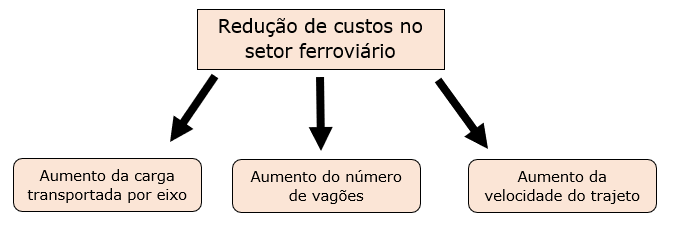
\includegraphics[width=1\textwidth]{reducao_custos}
		\caption{Principais formas de redução de custos no setor de transporte ferroviário.}
		\label{fig:reducao_custos}
	\end{figure}

	As formas de redução de custos mostradas na Fig. \ref{fig:reducao_custos} são benéficas no sentido de transportar mais carga em um menor período de tempo, mas também acarretam em maiores gastos com manutenções corretivas e preventivas, uma vez que carga e velocidade maiores implica em esforços na estrutura mecânica mais expressivos, especialmente no sistema roda-trilho.

	Os trilhos na via permanente e as rodas representam destacadamente o maior custo na manutenção do material rodante e a principal causa da retenção de vagões para a manutenção corretiva \cite{alves1997carga}.
	
	Aproveitando oportunidades nesse cenário, este estudo analisa o comportamento em desgaste por meio de ensaios de desgaste do tipo rolo contra disco de aços de rodas forjadas de mesma composição química e dureza, porém com diferentes microestruturas: perlítica e bainítica. Os resultados têm como objetivo sugerir o tipo de tratamento térmico mais adequado às aplicações propostas no transporte ferroviário e orientar fabricantes na indústria ferroviária e empresas operantes em ferrovias sobre qual microestrutura apresenta melhor comportamento em desgaste. 

	\section{Tribologia}
	
	A tribologia é a ciência que estuda os fenômenos de fricção, desgaste e lubrificação \cite{hutchings1992tribology}, assim, a análise da interação entre a roda e o trilho ferroviário também é escopo de estudo da tribologia.
	
	Em muitas circunstâncias, uma baixa fricção é desejada, como é o caso de juntas mecânicas, que demandam uma baixa força de fricção e em máquinas e equipamentos, que sob alta fricção leva à queda da eficiência geral. Mas no caso de freios e embreagens, por exemplo, a fricção é essencial para o funcionamento do sistema.
	
	A força de fricção pode ser definida como a resistência encontrada por um corpo ao se mover sobre outro \cite{hutchings1992tribology}. A fricção engloba duas importantes classes de movimento relativo: o rolamento e o deslizamento, conforme Fig. \ref{fig:rolamento_deslizamento}. A distinção entre os dois tipos de fricção é válida, mas os dois não são mutualmente exclusivos. Na prática não existe cada um desses fenômenos de forma ``pura'', geralmente os dois acontecem juntos em escalas diferentes.
	
	\begin{figure}[H]
		\centering
		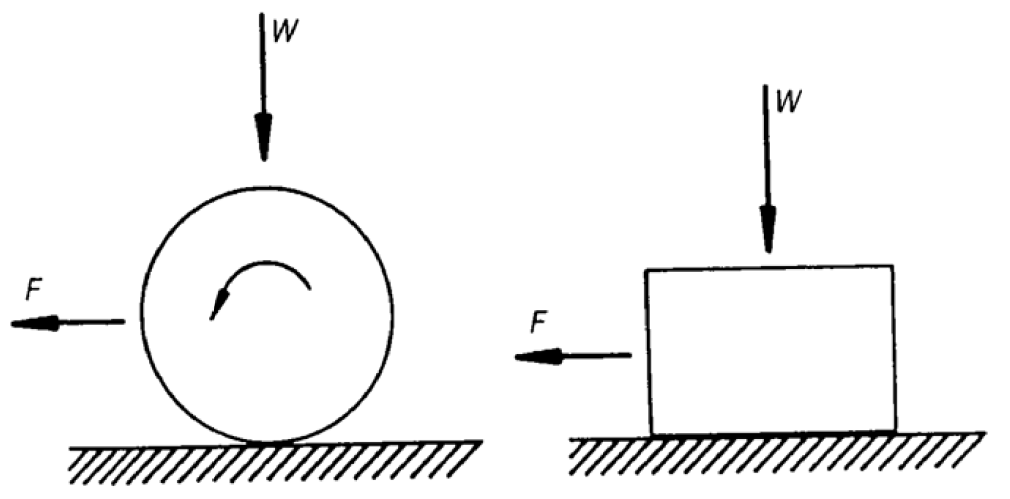
\includegraphics[width=1\textwidth]{rolamento_deslizamento}
		\caption{Uma força friccional, F, é necessária para causar o movimento por (a) rolamento ou (b) deslizamento. \cite{hutchings1992tribology}}
		\label{fig:rolamento_deslizamento}
	\end{figure}

	Muitas experimentações diferentes vem sendo testadas para estudar o desgaste por deslizamento e rolamento. Investigações em laboratório geralmente são feitas para simular aplicações práticas com diferentes variáveis e, assim, obter dados concisos de taxa de desgaste e coeficiente de fricção para cada caso. A Figura \ref{fig:testes_desgaste} mostra diferentes arranjos geométricos utilizados para análise de desgaste. 
	
	\begin{figure}[H]
		\centering
		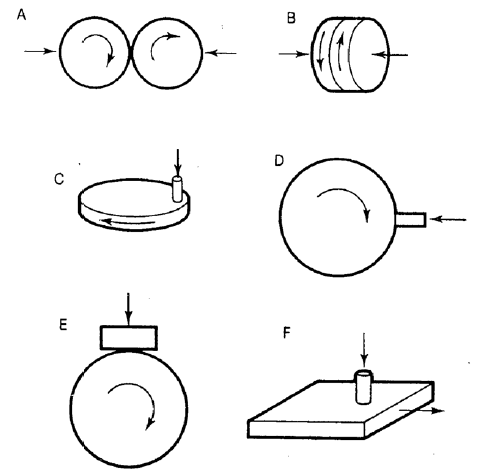
\includegraphics[width=0.8\textwidth]{testes_desgaste}
		\caption{Geometrias empregadas em testes de desgaste. \cite{hutchings1992tribology}}
		\label{fig:testes_desgaste}
	\end{figure}

	A palavra ``tribômetro'' é o termo utilizado para denominar um instrumento destinado a medir a fricção e desgaste de determinado material, sua geometria e arranjo dos elementos envolvidos podem ser tais como mostrados na Fig. \ref{fig:testes_desgaste}. 
	
	O tribômetro utilizado para a análise de desgaste de amostras de rodas ferroviárias foi um do tipo rolo contra disco. Neste tipo de tribômetro, o disco (ou contracorpo) é apoiado a uma base e gira sob rotação constante; já o rolo (ou corpo) é uma amostra de roda em miniatura, essa é forçada contra o disco através de uma carga, que a força a girar sobre o disco. Para a aplicação proposta neste trabalho, o rolo será da mesma composição da roda ferroviária, enquanto o disco será do mesmo material do trilho ferroviário. 
	
	Esse tribômetro, desenvolvido e fabricado na Universidade Federal de Juiz de Fora (UFJF), não oferece um tipo padronizado de teste, mas pode apontar dados importantes para a comparação de desempenho em desgaste para diferentes materiais. A Figura \ref{fig:tribometro_partes} mostra o tribômetro da UFJF.
	
	\begin{figure}[H]
		\centering
		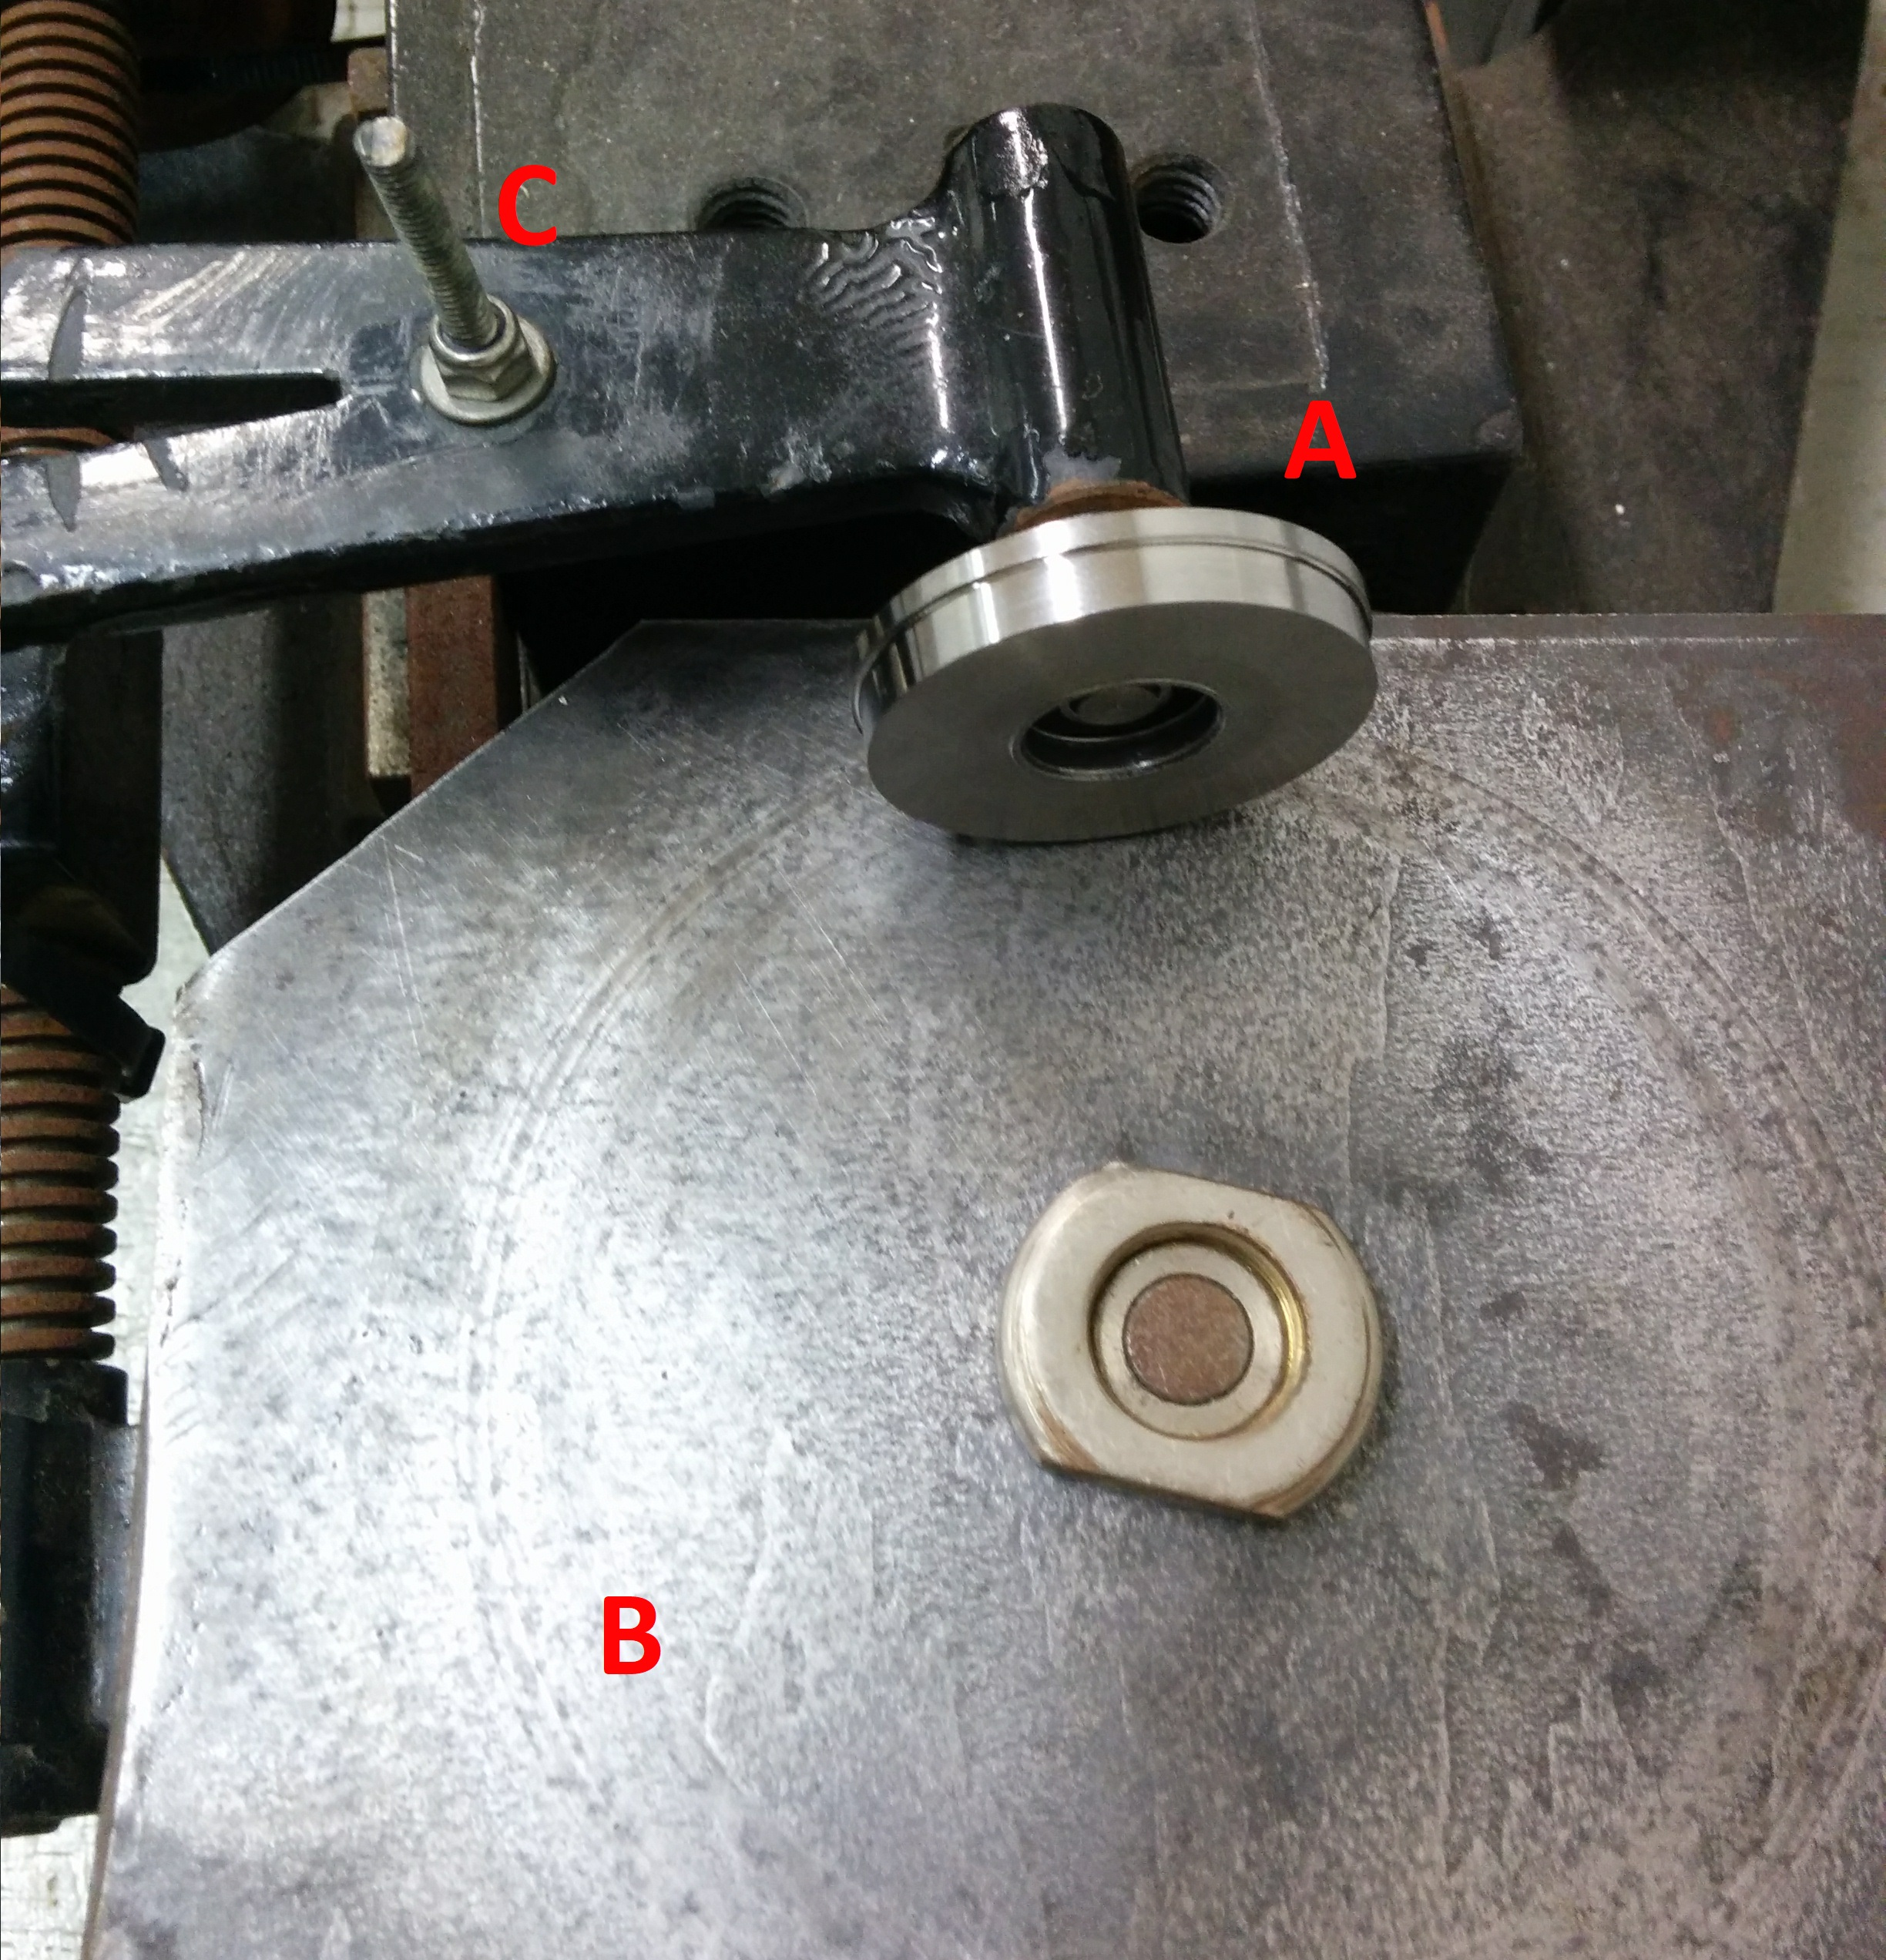
\includegraphics[width=0.9\textwidth]{tribometro_partes}
		\caption{O corpo (A) possui o mesmo material de uma roda ferroviária real, enquanto o contracorpo (B), o material de um trilho. O contato entre os dois é forçado por uma carga, que é apoiada sobre o pino de apoio de carga (C).}
		\label{fig:tribometro_partes}
	\end{figure}

	A taxa de desgaste é baseada a partir de uma simples teoria do desgaste por deslizamento: a equação de desgaste de Archard \cite{hutchings1992tribology}. Essa equação evidencia as principais variáveis que influenciam no desgaste; e também fornece uma maneira de descrever a severidade do desgaste, através de uma constante de desgaste. A Equação de Desgaste de Archard expressa a taxa de desgaste em função do volume total de material perdido com o atrito, da dureza do material mais macio e da carga aplicada para o contato entre eles. Essa equação será detalhadamente abordada na seção \ref{sec:revenido}.
	
	\pagebreak
	\section{Rodas ferroviárias}
	
	A pesquisa científica relativa ao transporte ferroviário no Brasil tem aumentado ultimamente devido a necessidade de redução de custos e aumento da competitividade no transporte de carga \cite{chaves2017rodas}. Cada vez mais pesquisas são realizadas a fim de se aprimorar o sistema roda-trilho. Diversas características são relevantes para a roda, dentre elas, pode-se destacar a composição, a geometria e os tratamentos térmicos utilizados na sua produção \cite{alves2000desgaste}, conforme ilustrado na Fig. \ref{fig:caracteristicas_roda}.
	
	\begin{figure}[H]
		\centering
		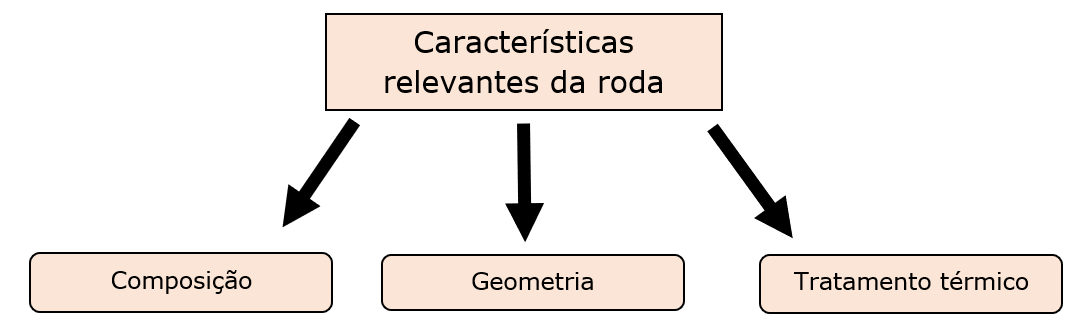
\includegraphics[width=1\textwidth]{caracteristicas_roda}
		\caption{Características relevantes da roda ao se analisar desgaste.}
		\label{fig:caracteristicas_roda}
	\end{figure}

	Uma das variáveis da Fig. \ref{fig:caracteristicas_roda} pode ser analisada separadamente através da fixação das outras duas variáveis. Por exemplo, pode-se fixar a composição e geometria a fim de se analisar o desempenho da roda no que diz respeito ao tratamento térmico adotado. 
	
	Um tratamento térmico é o processo de aquecimento e resfriamento visando modificar as propriedades do material para que sejam adequadas a diversas aplicações. Dentro dos tratamentos térmicos comuns na fabricação de rodas ferroviárias destaca-se o tratamento térmico de austêmpera, através do qual é obtida a microestrutura denominada bainita, que tem como característica a associação uma elevada dureza com uma alta tenacidade.
	
	No Brasil, as rodas ferroviárias são classificadas a partir das normas AAR M-107 e M-208 (Association of American Railroads) \cite{chaves2017rodas}. Em geral, as rodas ferroviárias tradicionais são de ligas ferro-carbono e possuem médio ou alto teor de carbono \cite{chaves2017rodas}. Nos trens brasileiros, as rodas mais utilizadas são as da AAR Classe C, que possuem um teor de carbono entre 0,67 \%p a 0,77\%p. A roda AAR Classe C é muito utilizada para o transporte de minérios, aplicação essa que impõe altas cargas por eixo sob baixas velocidades.
	
	\begin{figure}[H]
		\centering
		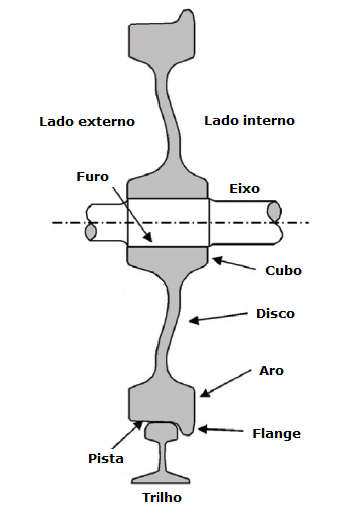
\includegraphics[width=0.25\textwidth]{roda}
		\caption{Designação das partes de uma roda ferroviária. \cite{okagata2013wheels} (adaptado)}
		\label{fig:roda}
	\end{figure}
	
	Para que o trilho e a roda assumam os formatos necessários, são utilizados diferentes tipos de processos de fabricação. Normalmente os trilhos são fabricados pelo processo de laminação e as rodas são forjadas a partir de lingotes ou fundidas em moldes de grafite pelo processo de baixa pressão \citep{paula2016desgaste}. Na Europa, as rodas forjadas são mais aplicadas em transportes com menor carga, como carros de passageiros; já nos Estados Unidos, as rodas fundidas são utilizadas em vagões de carga \citep{paula2016desgaste}.
	
	
	\section{Objetivos}
	
	Neste trabalho foram analisadas amostras materiais de rodas de aço de composição próxima à eutetóide, fabricadas pelo processo de fabricação de forjamento. Este estudo visa analisar o comportamento em desgaste a seco por meio de ensaios de desgaste do tipo rolo contra disco de aços de rodas forjadas de mesma composição química e dureza, porém com diferentes microestruturas: perlítica e bainítica. 
	
	Foram feitas análises de amostras de roda usinadas a partir do material de uma roda ferroviária real, feita de aço de composição próxima a eutetóide, muito utilizada nas aplicações de \textit{heavy haul}, como, por exemplo no transporte de minérios, onde há altas cargas, tensões e esforços mecânicos envolvidos. 
	
	Os resultados têm como objetivo sugerir o tipo de tratamento térmico mais adequado às aplicações propostas no transporte ferroviário e orientar fabricantes na indústria ferroviária e empresas operantes em ferrovias sobre qual microestrutura apresenta melhor comportamento em desgaste. 
	
	A utilização de rodas ferroviárias que sofrem menos falhas ou que têm seu tempo entre falhas reduzido auxiliaria no sentido de reduzir custos com manutenção corretiva e preventiva e, assim, aumentar a produtividade e competitividade no mercado de empresas atuando nesse setor.

	



	
\chapter{FUNDAMENTAÇÃO TEÓRICA}
	
\section{Ligas Ferro-Carbono}
\label{sec:liga_fe-c}

	Entre as ligas metálicas, as ligas ferro-carbono são as mais importantes e mais utilizadas na indústria. As ligas ferro-carbono podem ser subdivididas em aços e ferros fundidos. Ambos os componentes são materiais estruturais primários em qualquer sociedade tecnologicamente avançada.
	
	Os aços são muito suscetíveis a tratamentos térmicos, já que sua estrutura durante o tratamento podem sofrer profundas modificações, acarretando propriedades de alto significado para suas aplicações na indústria e na engenharia em geral \cite{chiaverini2003tratamentos}.
	
	Os ferros fundidos também reagem positivamente aos tratamentos térmicos, adquirindo propriedades importantes para diversas aplicações na engenharia.
	
	Os aços se diferenciam dos ferros fundidos pela quantidade de carbono presente em sua composição. Enquanto os aços possuem de 0\% a 2,14\% de C em massa, os ferros fundidos possuem concentração de 2,14\% a 6,7\% de C em massa. Embora uma liga de aço possa conter até 2,14\%p C, as concentrações para aplicações mais comuns na engenharia não costumam exceder 1,0\%p, o mesmo para os ferros fundidos comerciais, que, normalmente, possuem contração menor do que 4,5\%p C.
	
\subsection{Alotropia do ferro}

	O ferro é um elemento cuja forma (ou reticulado) cristalino é cúbico. O próprio ferro caracteriza-se por apresentar o fenômeno da alotropia (ou polimorfismo), que é a capacidade de possuir diferentes formas cristalinas para uma mesma composição. Suas formas principais são a cúbica de corpo  centrado (CCC) e cúbica de face centrada (CFC). A Figura \ref{fig:ccc_cfc} mostra diferentes estruturas do ferro.
	
	\begin{figure}[H]
		\centering
		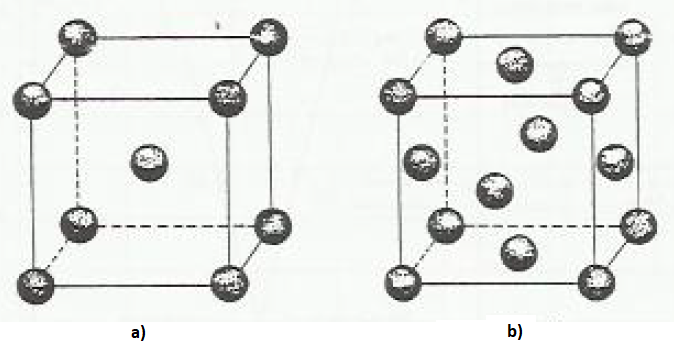
\includegraphics[width=0.7\textwidth]{ccc_cfc}
		\caption{Formas cristalinas do ferro. a) ferro $\alpha$ e ferro $\delta$. b) ferro $\gamma$. \cite{chiaverini2003tratamentos}}
		\label{fig:ccc_cfc}
	\end{figure}
	
	Quando há uma liga de ferro e carbono, também existem vários arranjos alotrópicos possíveis, conforme a Fig. \ref{fig:alotropia}. 
	
	\begin{figure}[H]
		\centering
		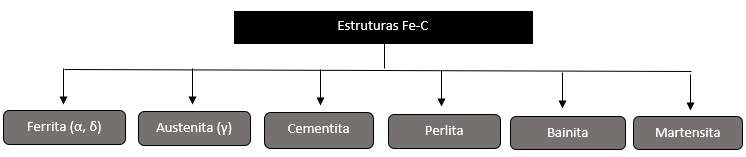
\includegraphics[width=1\textwidth]{alotropia}
		\caption{Algumas estruturas da liga $Fe-C$.}
		\label{fig:alotropia}
	\end{figure}

	Uma estrutura muito comum e importante nas transformações do ferro é a cementita ($Fe_3C$). Essa estrutura não apresenta reticulado cúbico como os do ferro $\alpha$ e $\gamma$. Ao invés disso, seu reticulado é ortorrômbico \cite{chiaverini2003tratamentos}, com 12 átomos de ferro e 4 átomos de carbono localizados nos interstícios dos átomos de ferro. A cementita ($Fe_3C$) é muito dura e, por isso, muito frágil, sendo sua resistência à tração também baixa devido a sua fragilidade. Já a ferrita (ferro $\alpha$) é dúctil e mole, com resistência relativamente baixa. A perlita, que é uma estrutura composta de lamelas alternadas de ferrita e cementita, possui propriedades intermediárias das fases $\alpha$ e $Fe_3C$. As propriedades experimentais de algumas microestruturas do aço estão expostas na Tab. \ref{tab:propriedades_aco}.
	
\begin{table}[H]
	\centering
	\caption{Propriedades mecânicas dos microconstituintes do aço. \cite{chiaverini2003tratamentos}}
	\resizebox{\textwidth}{!}{%
	\begin{tabular}{|c|c|c|c|c|}
		\hline
		\multirow{2}{*}{\textbf{Constituinte}} & \multicolumn{2}{c|}{\textbf{Limite de resistência à tração}} & \multicolumn{1}{c|}{\multirow{2}{*}{\textbf{Alongamento em 2''\newline{}(\%)}}} & \multirow{2}{*}{\textbf{Dureza Brinell}} \bigstrut\\
		\cline{2-3}               & \textbf{$kgf/mm^2$} & \textbf{MPa} &            &  \bigstrut\\
		\hline
		Ferrita    & 35         & 340        & cerca de 40 & 90 \bigstrut[t]\\
		Perlita    & 85         & 830        & cerca de 10 & 250-300 \\
		Cementita  & 3          & 30         & 0          & 650 \bigstrut[b]\\
		\hline
	\end{tabular}%
	}
	\label{tab:propriedades_aco}%

\end{table}%

	Além dessas, existem também as fases bainita e martensita, ilustradas na Fig. \ref{fig:alotropia}. Como ocorre na perlita, a microestrutura da bainita consiste nas fases ferrita e cementita, mas os arranjos são diferentes, já a martensita é obtida através de uma transformação polimórfica da austenita para estrutura tetragonal de corpo centrado (TCC). Essas duas microestruturas são obtidas através de tratamentos térmicos.	
	

\subsection{Diagrama Ferro - Carbeto de Ferro ($Fe-Fe_3C$)}

	O diagrama de fases da liga ferro-carbono é apresentado na Fig. \ref{fig:ferro_carbono}, onde a parte à esquerda representa ferro puro e a parte à direita representa uma concentração de 6,70\% de C em massa ou uma concentração pura de cementita ($Fe_3C$). 

	
	
	\begin{figure}[H]
		\centering
		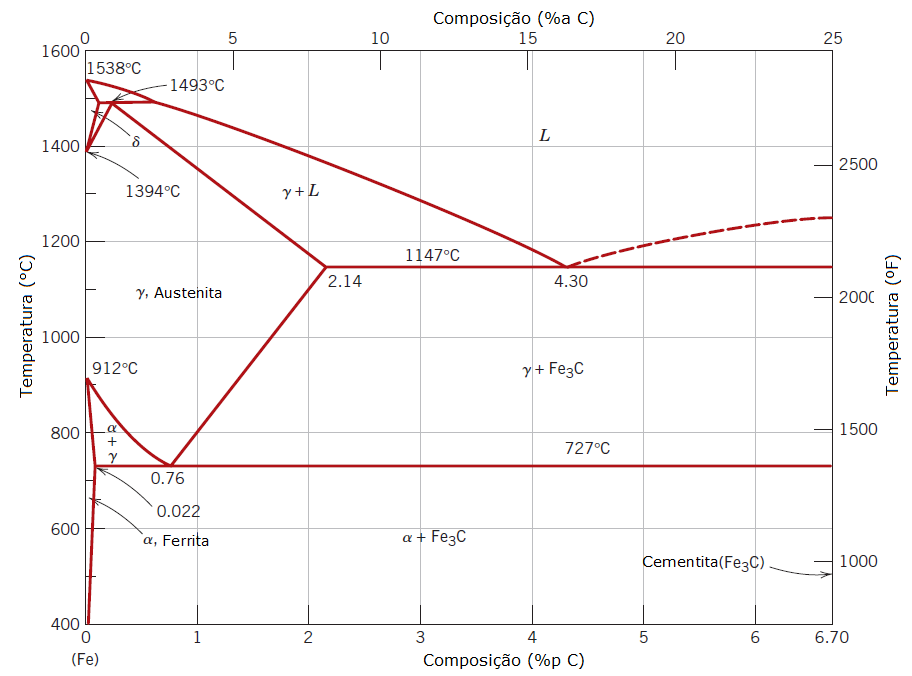
\includegraphics[width=1\textwidth]{ferro_carbono}
		\caption{Diagrama $Fe-Fe_3C$. \cite{callister2011materials}}
		\label{fig:ferro_carbono}
	\end{figure}

	As principais fases que podem ser observadas a partir da Fig. \ref{fig:ferro_carbono} são:

	\begin{itemize}
		\item Ferro $\alpha$ ou ferrita;
		\item Ferro $\gamma$ ou austenita;
		\item Ferrita $\delta$;
		\item Fase líquida (L);
		\item Cementita ou carbeto de ferro ($Fe_3C$).
	\end{itemize}

	A ferrita $\alpha$ possui baixas concentrações de carbono, com solubilidade máxima de 0,022\%p. Embora presente em concentrações relativamente baixas, o carbono presente na ferrita $\alpha$ influencia de maneira significativa em suas propriedades mecânicas \cite{callister2011materials}. Essa fase ferro-carbono é relativamente dúctil.
	
	A austenita, ou ferro $\gamma$, possui solubilidade máxima de carbono de 2,14\%p, que é aproximadamente 100 vezes maior do que a máxima solubilidade da ferrita $\alpha$, isso se deve ao fato de que as posições intersticiais na estrutura CFC são maiores e, portanto, podem acomodar mais átomos de carbono.
	
	A Figura \ref{fig:ferrita_austenita} mostra fotomicrografias das fases ferrita $\alpha$ e austenita $\gamma$.
	
	\begin{figure}[H]
		\centering
		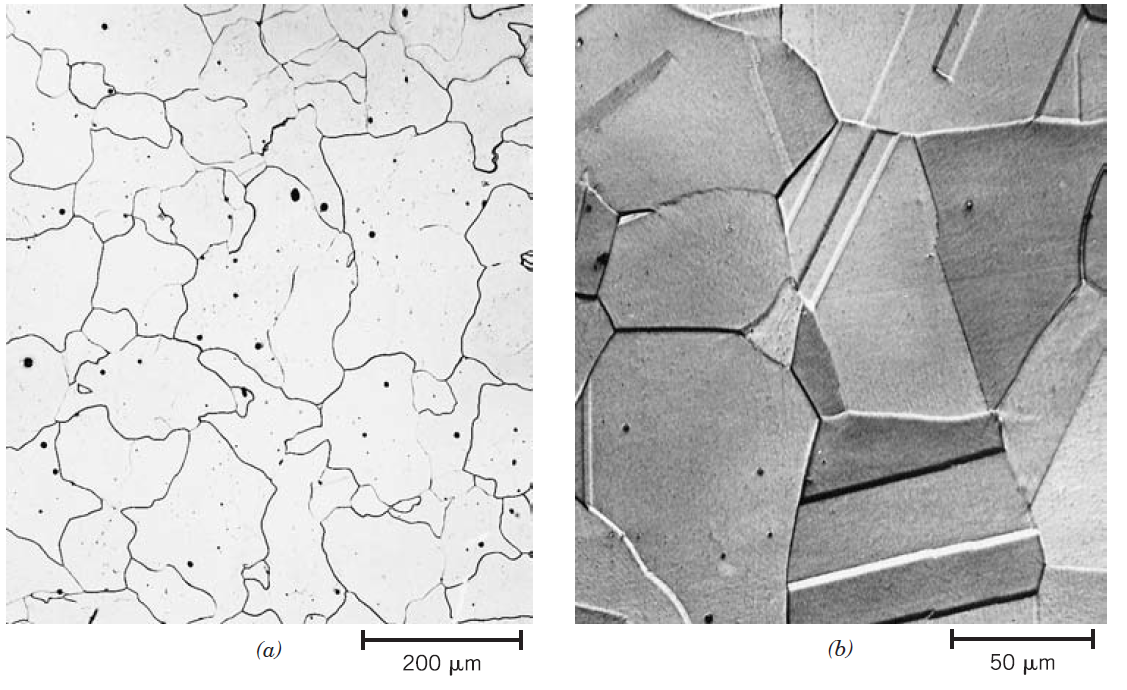
\includegraphics[width=1\textwidth]{ferrita_austenita}
		\caption{Fotomicrografia da ferrita $\alpha$ (a) e da austenita $\gamma$ (b). \cite{callister2011materials}}
		\label{fig:ferrita_austenita}
	\end{figure}
	
	A ferrita $\delta$ é virtualmente idêntica à ferrita $\alpha$, porém em uma faixa de temperatura maior.
	
	A cementita ($Fe_3C$) é formada ao se exceder o limite de solubilidade da ferrita $\alpha$ à temperatura abaixo de 727$^{\circ}$C, como pode ser observar na Fig. \ref{fig:ferro_carbono}. Mecanicamente, a cementita é muito dura e frágil \cite{callister2011materials}, o que sugere que quanto maior a concentração de carbono na liga ferro-carbono maior a fragilidade do material.
	
	No diagrama $Fe-Fe_3C$, existe um ponto invariante eutetóide (ou ponto E), que corresponde à menor temperatura de equilíbrio entre as fases ferrita $\alpha$ e austenita $\gamma$, correspondendo a cerca de 0,76\% de carbono à 727$^{\circ}$C. O termo eutético se remete ao equilíbrio entre fases líquida e sólida, o sufixo ``oide'' é utilizado para indicar o equilíbrio entre fases sólidas.

\pagebreak

\subsection{Resfriamento lento}
	
	Uma composição eutetóide de uma liga é a composição sob a qual tem-se a menor temperatura de equilíbrio entre as fases ferrita e austenita. Esta composição na liga ferro-carbono equivale a 0,76\%p C, o que se assemelha à composição de um aço SAE 1080. O ponto E na Fig. \ref{fig:eutetoide} representa o ponto eutetóide no diagrama ferro - carbeto de ferro.
	
	\begin{figure}[H]
		\centering
		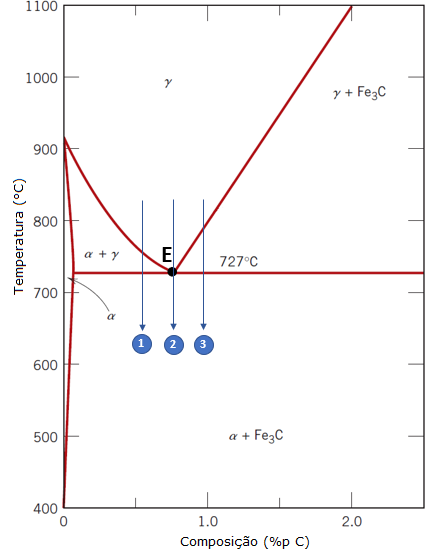
\includegraphics[width=0.7\textwidth]{eutetoide}
		\caption{Resfriamento hipoeutetóide (1), eutetóide (2) e hipereutetóide (3). \cite{callister2011materials} (adaptado)}
		\label{fig:eutetoide}
	\end{figure}

	Considerando o resfriamento lento de uma liga eutetóide, ela é resfriada desde a fase austenítica (por exemplo, à 800$^{\circ}$C) e a mudança de fase irá ocorrer ao se atingir a temperatura eutetóide (727$^{\circ}$C), vide Fig. \ref{fig:eutetoide}. Ao se resfriar lentamente até abaixo da temperatura eutetóide, a microestrutura se transforma em camadas alternadas (ou lamelas) das fases $\alpha$ e $Fe_3C$, que se formam simultaneamente durante a transformação. Tal resfriamento é esquematizado pela linha (2) na Fig. \ref{fig:eutetoide}.
	
	Essa microestrutura composta de lamelas alternadas de ferrita e cementita é denominada perlita. A Figura \ref{fig:perlita} mostra o arranjo da microestrutura perlítica. As camadas claras e mais grossas são a fase ferrita, enquanto a fase cementita aparece como finas lamelas de coloração mais escura. Mecanicamente, a perlita apresenta propriedades intermediárias entre a ferrita macia e dúctil, e a cementita dura e frágil \cite{callister2011materials}.
	
	\begin{figure}[H]
		\centering
		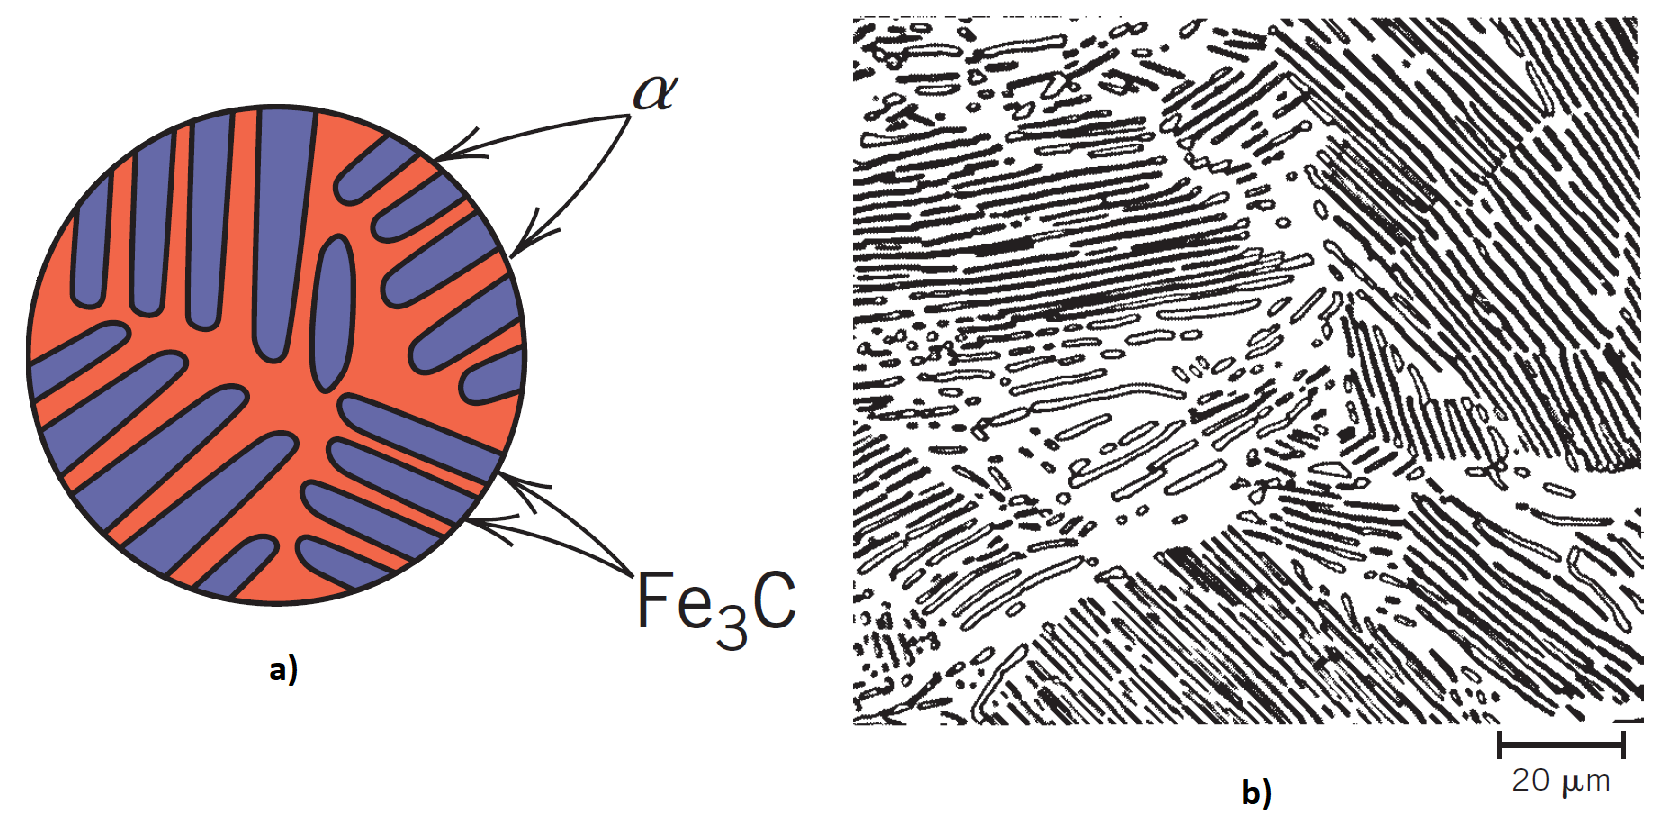
\includegraphics[width=1\textwidth]{perlita}
		\caption{a) Esquema ilustrativo da microestrutura perlítica. b) Fotomicrografia de um aço eutetóide mostrando a microestrutura da perlita. \cite{callister2011materials} (adaptado)}
		\label{fig:perlita}
	\end{figure}

	As composições de ligas hipoeutetóides são composições de carbono inferiores a da eutetóide e estão à esquerda do ponto E na Fig. \ref{fig:eutetoide}. O resfriamento de ligas hipoeutetóides é ilustrado pela linha (1) na Fig. \ref{fig:eutetoide}.
	
	Ao se resfriar a partir da fase austenítica, o aço passa pela fase $\alpha+\gamma$, onde essas duas fases irão coexistir. Quando a temperatura é reduzida imediatamente abaixo da temperatura eutetóide, toda a fase $\gamma$ da fase anterior se transformará em perlita, enquanto a fase $\alpha$ já existente permanecerá na nova fase como ferrita proeutetóide. A Figura \ref{fig:perlita_hipo} mostra o arranjo da microestrutura composta por perlita e ferrita proeutetóide.
	
	\begin{figure}[H]
		\centering
		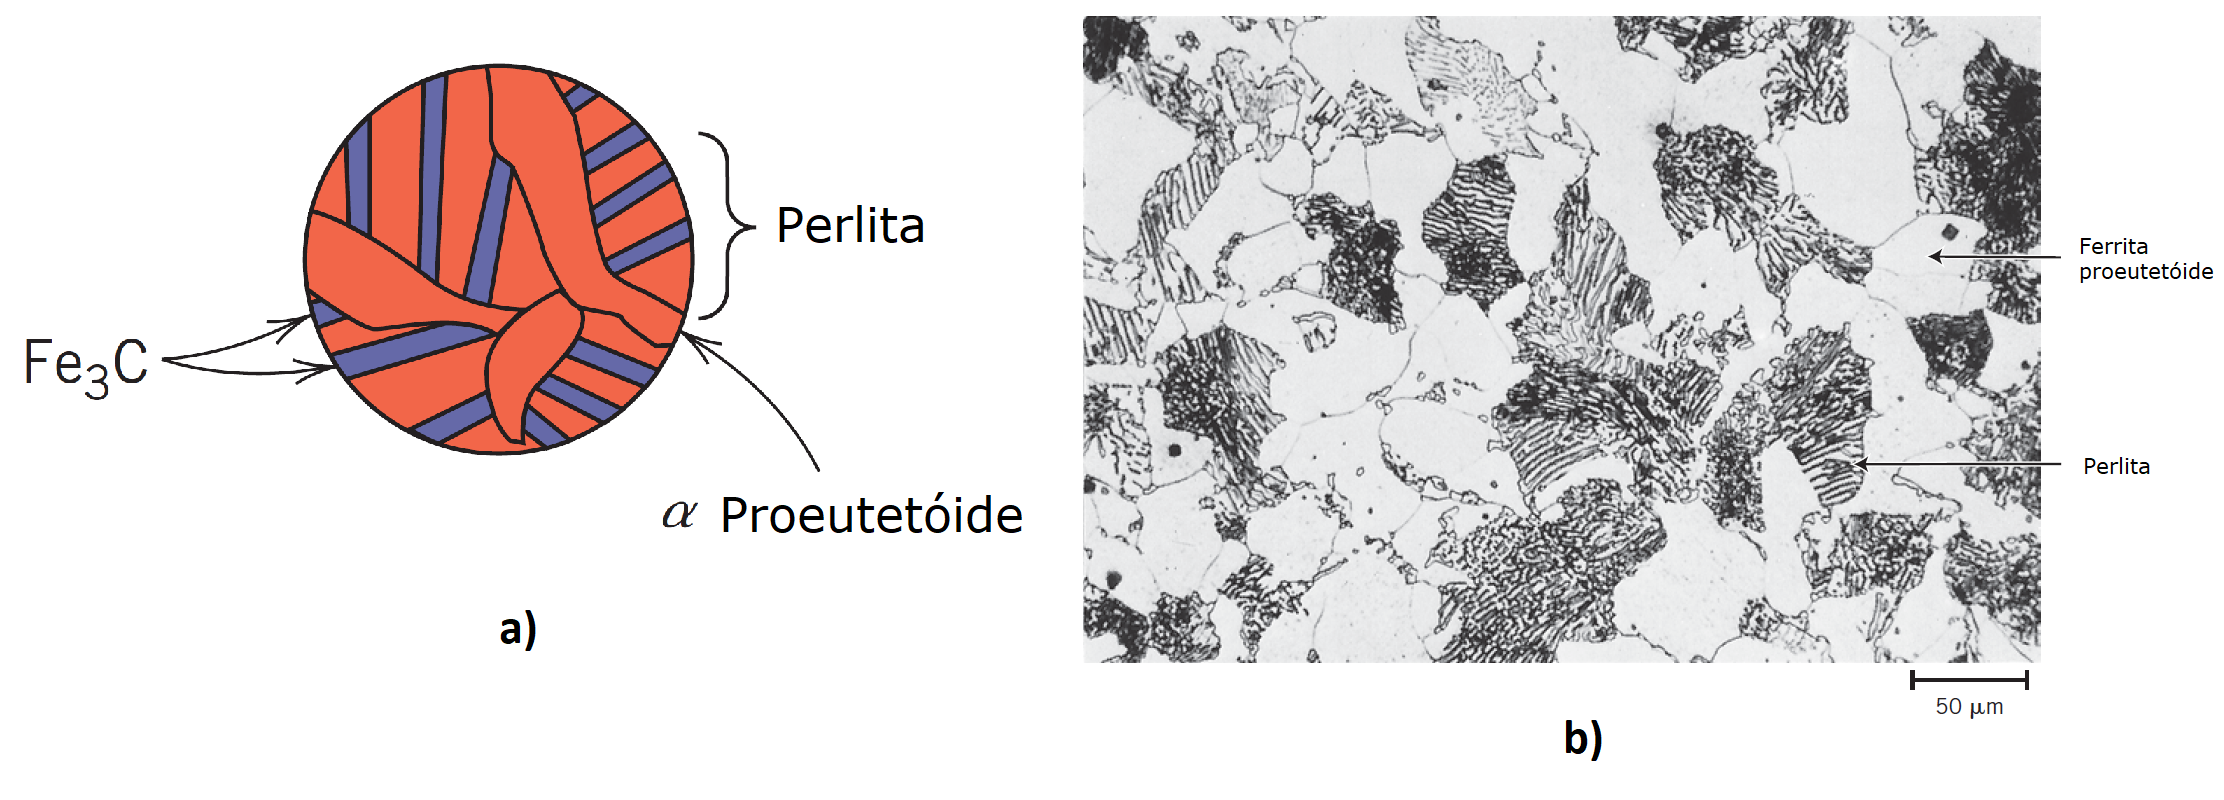
\includegraphics[width=1\textwidth]{perlita_hipo}
		\caption{a) Esquema ilustrativo da microestrutura composta por perlita e ferrita proeutetóide. b) Fotomicrografia de um aço com 0,38\%p C mostrando sua microestrutura. \cite{callister2011materials} (adaptado)}
		\label{fig:perlita_hipo}
	\end{figure}

	Já para microestruturas das ligas de composição hipereutetóide (acima de 0,76\%p C), o resfriamento e transformação de microestruturas são representados pela linha (3) na Fig. \ref{fig:eutetoide}. Com o resfriamento a partir da fase austenítica pura, o aço passa pela fase $\gamma + Fe_3C$, onde a fase cementita começa a se formar ao longo dos contornos de grão iniciais da fase $\gamma$. Esta cementita formada é denominada cementita proeutetóide, pois ela continua em sua forma mesmo após o posterior resfriamento até abaixo da temperatura eutetóide, enquanto a fase austenítica restante se transforma em perlita. A Figura \ref{fig:perlita_hiper} mostra o arranjo da microestrutura composta por perlita e cementita proeutetóide.
	
	\begin{figure}[H]
		\centering
		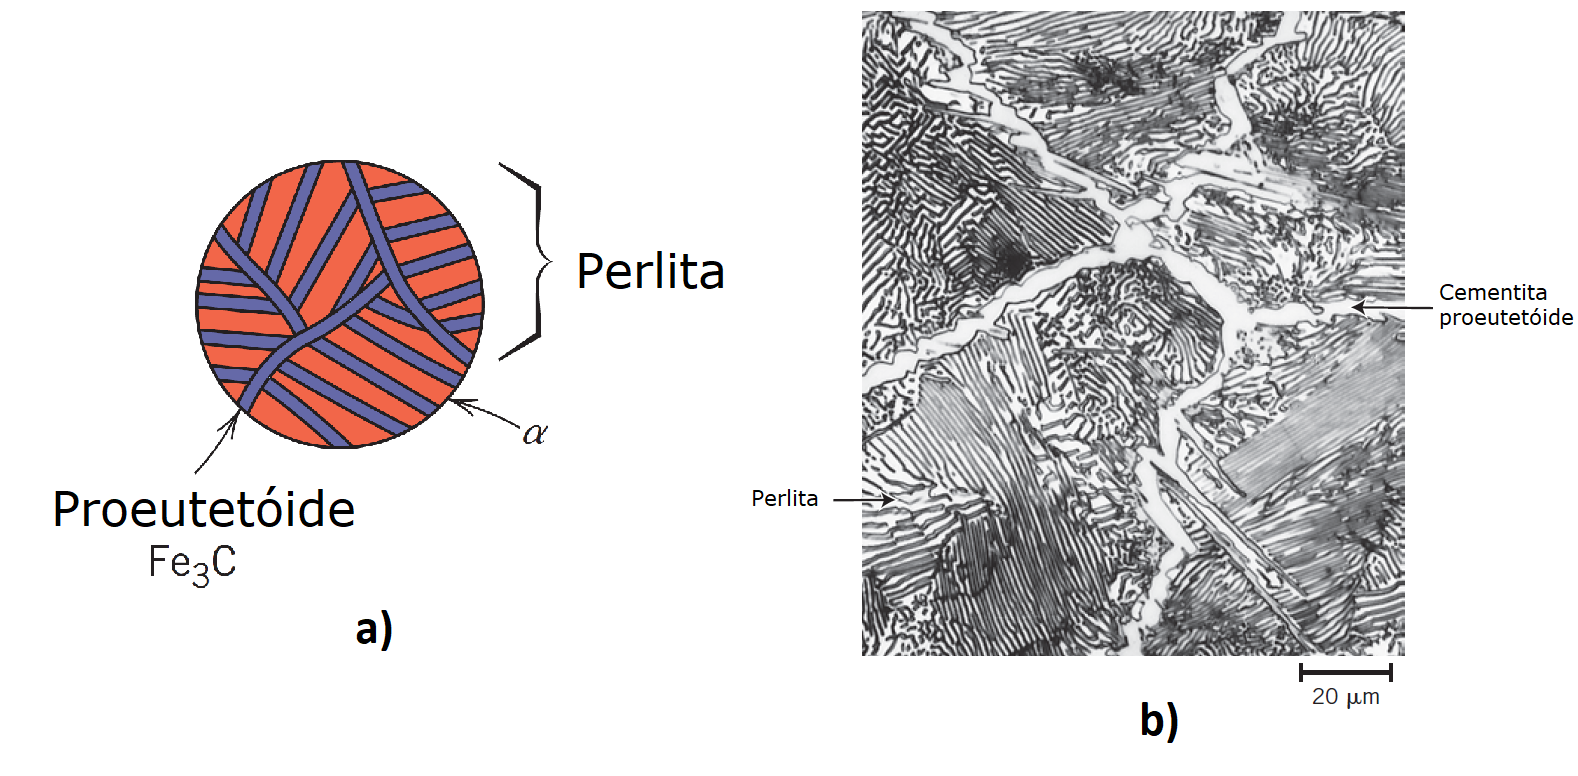
\includegraphics[width=1\textwidth]{perlita_hiper}
		\caption{a) Esquema ilustrativo da microestrutura composta por perlita e cementita proeutetóide. b) Fotomicrografia de um aço com 1,40\%p C mostrando sua microestrutura. \cite{callister2011materials} (adaptado)}
		\label{fig:perlita_hiper}
	\end{figure}
	
\pagebreak
\section{Tratamentos térmicos em aços}	

	Tratamentos térmicos são um conjunto de operações objetivando a modificação microestrutural e, consequentemente, as propriedades de um determinado material. 

	Em aços, tratamentos térmicos são muito aplicados, uma vez que essas operações podem modificar significativamente as características de um elemento e permitem, assim, que as ligas sejam adequadas a diversas aplicações na engenharia.

	Os tratamentos térmicos são realizados em operações que incluem o aquecimento, resfriamento e manutenção de temperaturas sob condições ideais controladas.

	Alguns dos principais tipos de tratamento térmico aplicado aos aços são:
\begin{enumerate}[label=(\alph*)]
	\item Recozimento;
	\item Normalização;
	\item Têmpera;
	\item Austêmpera;
	\item Martêmpera;
	\item Revenimento.
\end{enumerate}

	Além desses, existem também tratamentos termoquímicos, em que a composição química da região superficial do material é modificada intencionalmente, como é o caso da cementação, nitretação, cianetação, carbonitretação e outros.
	
	Ao longo desta seção, são abordados principalmente os tratamentos de austêmpera e revenimento, necessários para o entendimento do presente estudo.

	
\subsection{Transformação isotérmica}

	As transformações microestruturais explanados na seção \ref{sec:liga_fe-c} acontecem para resfriamentos lentos, ou seja, o tempo para a transformação estrutural é alto. Porém, há outro fator que influencia na microestrutura final após o tratamento térmico que é a velocidade de resfriamento, que está diretamente associado à taxa de transformação estrutural que esse aço irá apresentar.
	
	O aumento da velocidade de resfriamento altera as condições de formação dos constituintes normais a partir da austenita. Essa formação é baseada na movimentação dos átomos do aço por difusão \cite{chiaverini2003tratamentos}. Os microconstituintes resultantes de diferentes velocidades de resfriamento possuem características distintas e também propriedades e aplicações diferentes na indústria.
	
	O diagrama que mostra os microconstituintes gerados a partir de taxas de resfriamento elevadas é mostrado na Fig. \ref{fig:isotermico}. Esse diagrama é chamado de diagrama TTT (transformação-tempo-temperatura) ou diagrama C (devido à forma de sua curva).
	
	\begin{figure}[H]
		\centering
		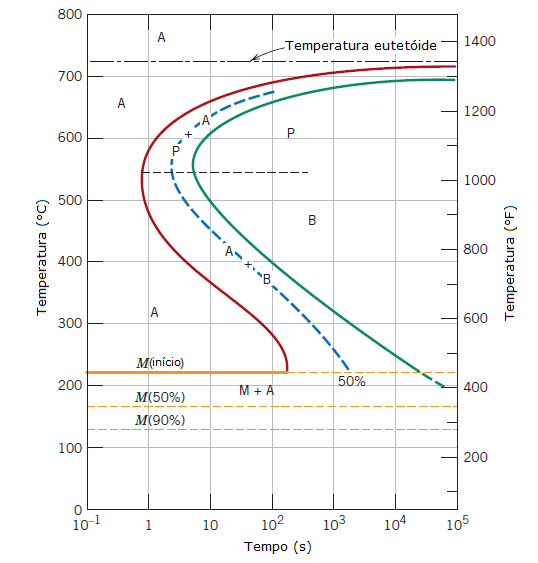
\includegraphics[width=0.9\textwidth]{isotermico}
		\caption{Diagrama TTT de um aço eutetóide. As letras A, P, B e M representam, respectivamente, as microestruturas austenita, perlita, bainita e martensita. \cite{callister2011materials}}
		\label{fig:isotermico}
	\end{figure}

	No diagrama da Fig. \ref{fig:isotermico}, o eixo vertical representa a temperatura do aço a ser tratado. Em um tratamento isotérmico, o aço é aquecido até além da temperatura de austenitização e, após isso, é resfriado em um banho, geralmente de sais fundidos, à temperatura até a qual se deseja resfriar o aço. O eixo horizontal representa o tempo, em escala logarítmica, do processo de resfriamento. As curvas vermelhas e verdes representam, respectivamente, o início e o fim da transformação da austenita para a perlita ou bainita, enquanto que as curvas amarelas representam as fases de transformação da austenita para a martensita.
	
	É interessante notar que, para um aço eutetóide, a obtenção de perlita deve ser feita com o aquecimento até além da temperatura de austenitização (727$^\circ$C) e o resfriamento a temperaturas acima de 540$^\circ$C, ou seja, acima do ``nariz'' ou ``joelho'' do diagrama da Fig. \ref{fig:isotermico}, como comumente é referenciada essa curva. E o aço deve ser mantido a esta temperatura por tempo suficiente para que a transformação comece (linha vermelha, sobre o ponto C) e então seja concluída (linha verde, sobre o ponto D). A Figura \ref{fig:formacao_perlita} ilustra através das linhas pretas (ABCD) o esquema de resfriamento para obtenção de perlita.
	
	\begin{figure}[H]
		\centering
		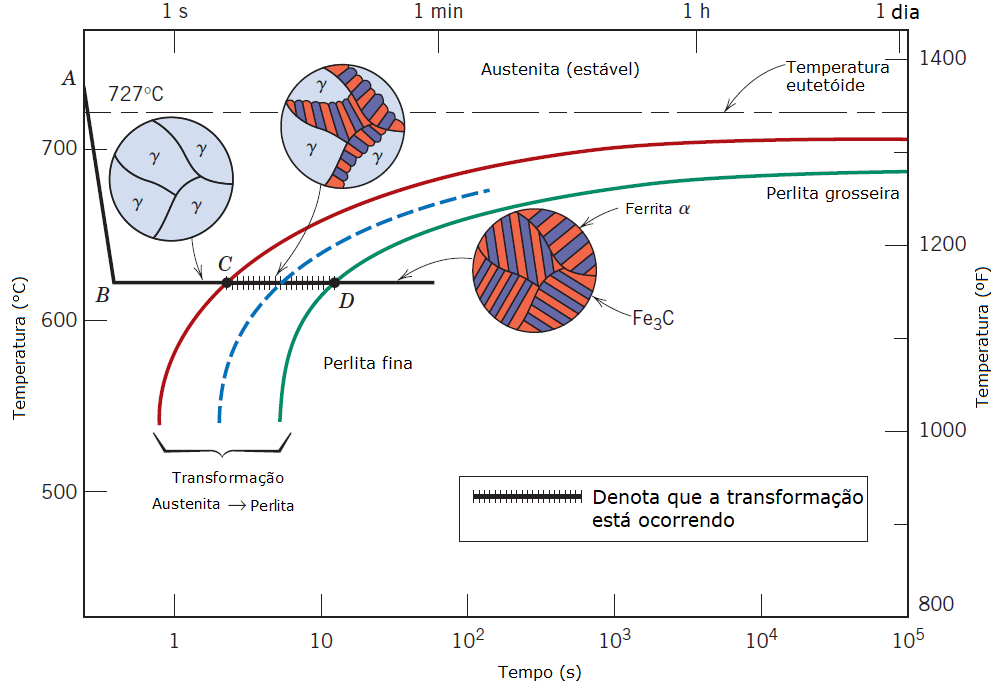
\includegraphics[width=0.95\textwidth]{formacao_perlita}
		\caption{Diagrama de transformação isotérmica para uma liga ferro-carbono eutetóide, com superposição da curva para um tratamento térmico isotérmico (ABCD). As microestruturas antes, durante e depois da transformação da austenita em perlita são mostradas. \cite{callister2011materials}}
		\label{fig:formacao_perlita}
	\end{figure}
	
	Para a formação de bainita, o aço deve ser aquecido até além da temperatura de austenitização (727$^\circ$C) e resfriado à temperatura abaixo da curva do ``nariz'' (aproximadamente 540$^\circ$C), mantendo tal temperatura por tempo suficiente para que haja a transformação total da austenita em bainita. 
	
	Como a troca de calor não é instantânea e há um tempo de resfriamento do metal do banho de sais, é importante observar que, para a formação plena da estrutura bainítica, a taxa de resfriamento deve ser rápida o suficiente para que a linha de resfriamento não cruze o ``nariz'' do diagrama, situação na qual haveria uma parcial transformação da austenita em perlita. A Fig. \ref{fig:resfriamento_ttt} mostra diferentes taxas de resfriamento em sobreposição a um diagrama TTT.
	
	\begin{figure}[H]
		\centering
		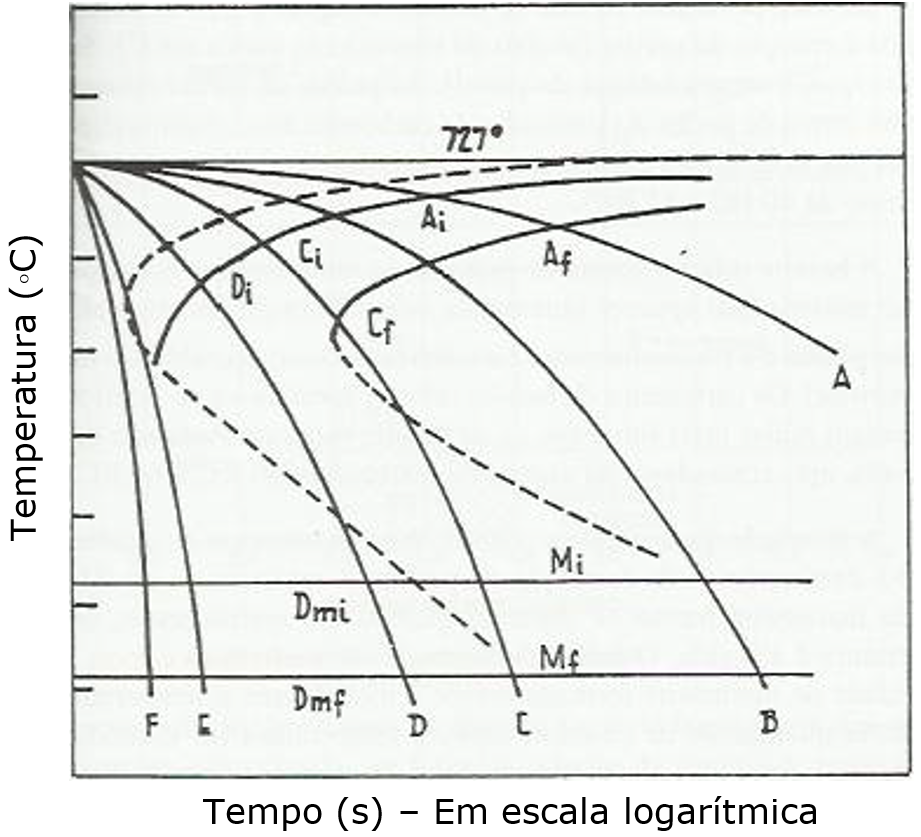
\includegraphics[width=0.75\textwidth]{resfriamento_ttt}
		\caption{Superposição de curvas de resfriamento no diagrama de transformação para resfriamento contínuo. \cite{chiaverini2003tratamentos}}
		\label{fig:resfriamento_ttt}
	\end{figure}

	O outro microconstituinte no diagrama da Fig. \ref{fig:isotermico} é a martensita, que é formada quando as ligas ferro-carbono austenitizadas são resfriadas bruscamente (ou temperadas) até um temperatura relativamente baixa. Na transformação para a martensita, a austenita (com estrutura CFC) sofre uma transformação polimórfica para uma estrutura martensita tetragonal de corpo centrado (TCC) \cite{callister2011materials}.




\subsection{Austêmpera}
	Austêmpera é a transformação isotérmica de uma liga ferrosa a temperatura abaixo daquela em que há a formação de perlita e acima da formação de martensita. Esse tratamento visa obter a estrutura bainita no aço, estrutura essa que não é tão dura quanto a martensita e ainda é mais tenaz.
	
	A austêmpera de aços oferece a potencial vantagem do aumento da ductilidade, dureza, tenacidade e resistência do aço para uma dada dureza \cite{asm1991heat}.
	
	Um aço é austemperado através dos seguintes os passos:
	
	\begin{enumerate}
		\item Aquecer o material até a temperatura de austenitização, geralmente entre 790$^{\circ}$C e 915$^{\circ}$C;
		\item Mergulhar em um banho em temperatura constante, geralmente entre 260$^{\circ}$C e 400$^{\circ}$C;
		\item Manter sob tal temperatura até que o material sofra transformação isotérmica no banho;
		\item Resfriar sob temperatura ambiente.
	\end{enumerate}

	A Figura \ref{fig:formacao_bainita} mostra, através do diagrama de transformação isotérmica, o tratamento térmico da austêmpera.
	
	\begin{figure}[H]
		\centering
		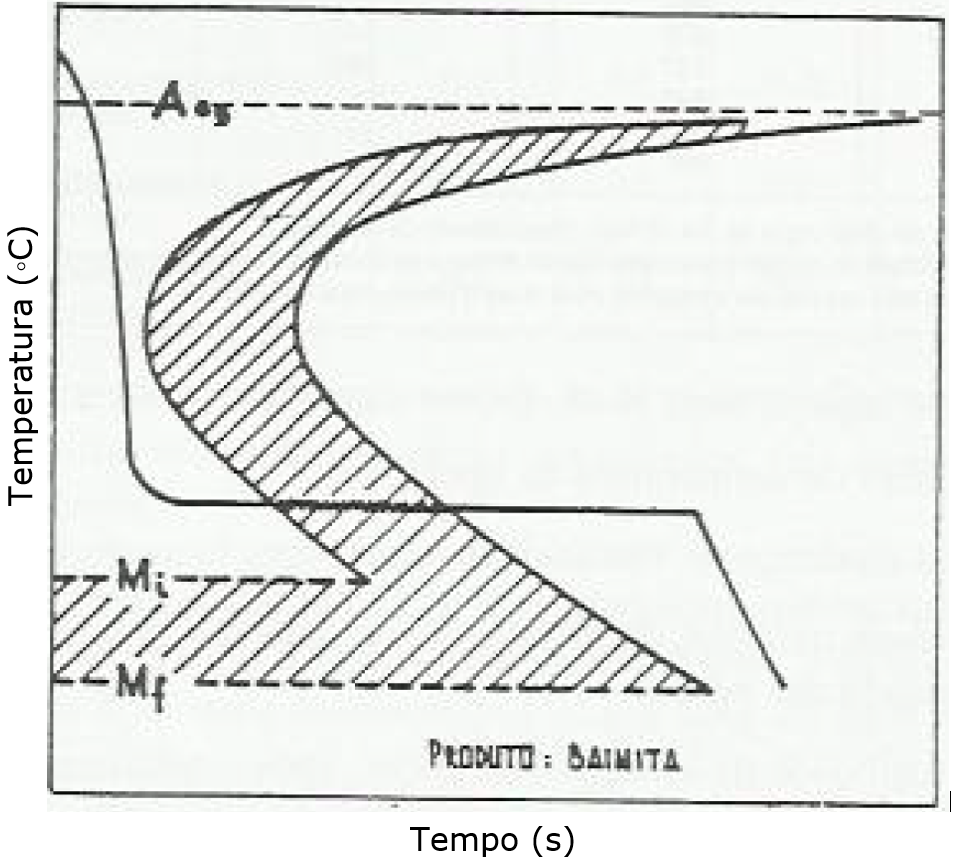
\includegraphics[width=0.85\textwidth]{formacao_bainita}
		\caption{Representação esquemática do diagrama de transformação isotérmica para a austêmpera, com formação de bainita. \cite{chiaverini2003tratamentos}}
		\label{fig:formacao_bainita}
	\end{figure}

	Para a eficácia austêmpera, o metal deve ser resfriado da temperatura de austenitização para a temperatura do banho de austêmpera rápido suficiente para que não ocorra transformação de austenita durante o resfriamento e então deve ser mantida no banho de austêmpera por tempo suficiente para que se tenha certeza que houve a total transformação da austenita em bainita.

	O aspecto micrográfico da bainita está representado na Fig. \ref{fig:bainita_bib}.
	
	\begin{figure}[H]
		\centering
		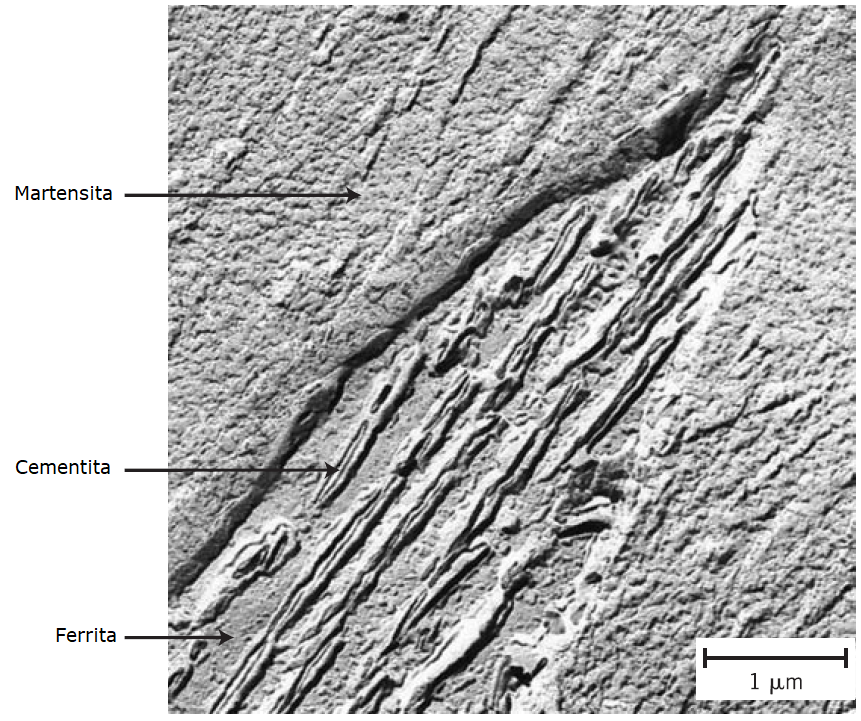
\includegraphics[width=0.75\textwidth]{bainita_bib}
		\caption{Micrografia mostrando a estrutura da bainita. O grão de bainita aparece do canto inferior esquerda ao canto superior direito; se consiste de partículas de $Fe_3C$ alongadas e em forma de agulhas dentro de uma matriz de ferrita. \cite{callister2011materials}}
		\label{fig:bainita_bib}
	\end{figure}

	Os aços mais indicados para a operação de austêmpera devem possuir elevado teor de carbono e também determinados elementos de liga que desloquem as curvas em C para a direita \cite{chiaverini2003tratamentos}, a fim de se evitar que a curva de resfriamento corte a curva de início de transformação austenítica.
	
	O meio de resfriamento da austêmpera mais comum é o banho de sais fundidos, constituído de uma mistura de nitrato de sódio e nitrato de potássio \cite{chiaverini2003tratamentos}. Esse meio de resfriamento é bastante utilizado, pois \cite{asm1991heat}:
	
	\begin{itemize}
		\item Transfere calor rapidamente;
		\item Elimina o problema da barreira de vapor ao redor do material durante o estágio inicial do banho;
		\item Sua viscosidade é uniforme em uma alta faixa de temperaturas;
		\item Sua viscosidade é baixa a temperaturas de austêmpera (próxima à da água a temperatura ambiente), reduzindo, assim, perdas de arrasto;
		\item É estável nas temperaturas de operação e é solúvel em água, facilitando, assim, a limpeza subsequente.
	\end{itemize}

	A austêmpera é geralmente usada como substituta da têmpera convencional para se obter características mecânicas desejáveis (maior ductilidade e tenacidade), para melhorar a resistência ao desgaste a uma dada dureza e para aumentar a resistência à falha frágil \cite{asm1991heat}. Além disso, em algumas aplicações, a austêmpera é mais viável economicamente do que a têmpera convencional \cite{asm1991heat}.


\subsection{Revenido}
	Esse tratamento consiste no reaquecimento das peças temperadas a temperaturas situadas abaixo da linha inferior de transformação do aço. A Figura \ref{fig:revenido} mostra um diagrama de uma operação de revenido realizada após uma têmpera.

	\begin{figure}[H]
		\centering
		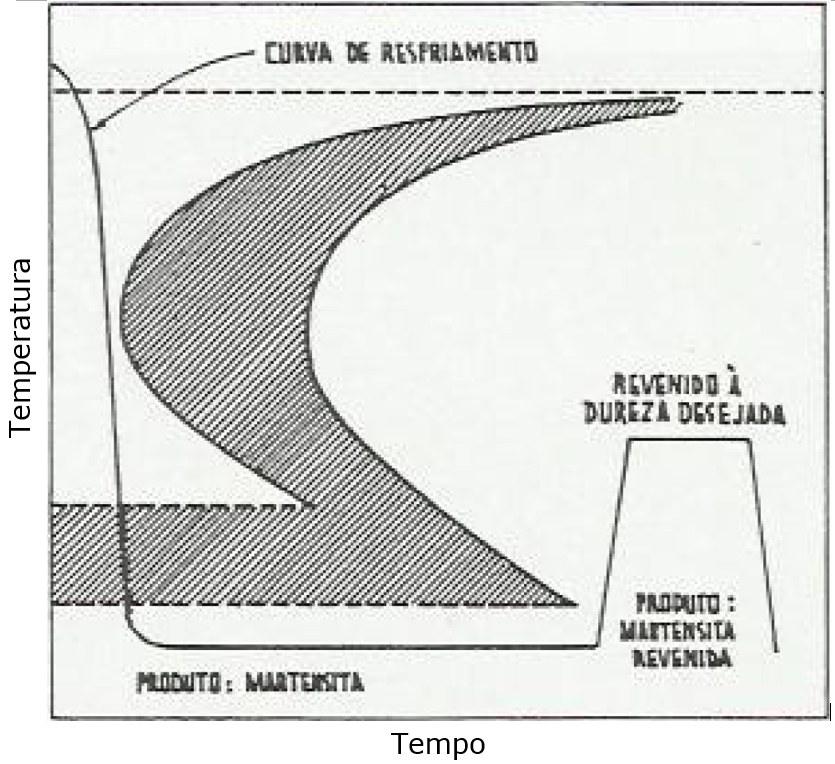
\includegraphics[width=0.85\textwidth]{revenido}
		\caption{Diagrama esquemático representativo da operação de têmpera e revenido. \cite{chiaverini2003tratamentos}}
		\label{fig:revenido}
	\end{figure}

	O revenido é conduzido normalmente em temperaturas entre 250$^{\circ}$C e 650$^{\circ}$C \cite{callister2011materials} e tem o objetivo de aliviar ou remover as tensões introduzidas durante o tratamento de têmpera e corrigir a dureza e a fragilidade da peça, aumentando resistência, desgaste e tenacidade, minimizando os efeitos térmicos e mecânicos provocados pelo cisalhamento da estrutura austenitizada \cite{vale2016tratamento}. O revenido melhora a ductilidade e a tenacidade da martensita.
	
	O revenido pode também reduzir consideravelmente a dureza de uma liga ferro-carbono, como pode se observar pela Fig. \ref{fig:martensita_revenida} e \ref{fig:dureza_resistencia_revenido}.
	
	\begin{figure}[H]
		\centering
		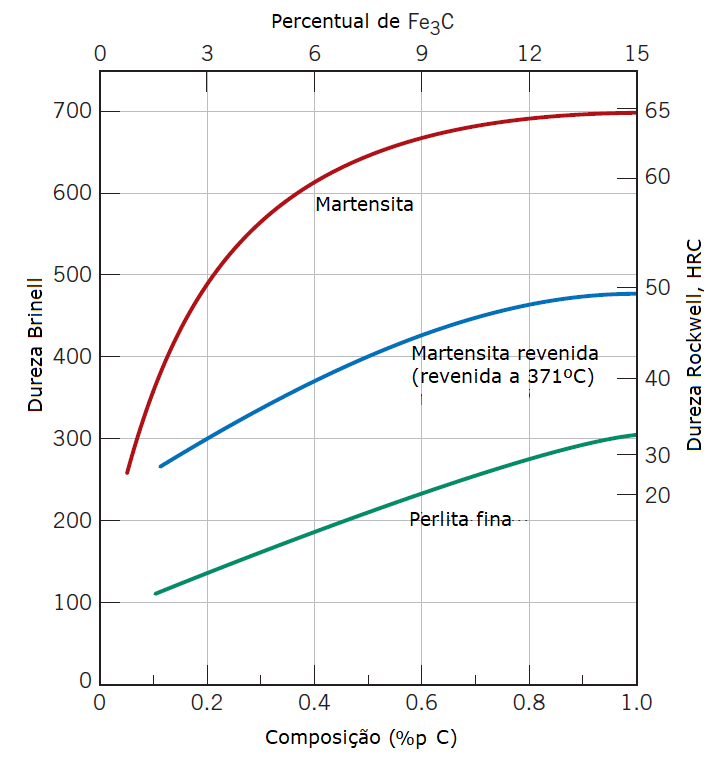
\includegraphics[width=0.85\textwidth]{martensita_revenida}
		\caption{Dureza em função da concentração de carbono para a martensita pura, martensita revenida e perlita fina. \cite{callister2011materials}}
		\label{fig:martensita_revenida}
	\end{figure}

	\begin{figure}[H]
		\centering
		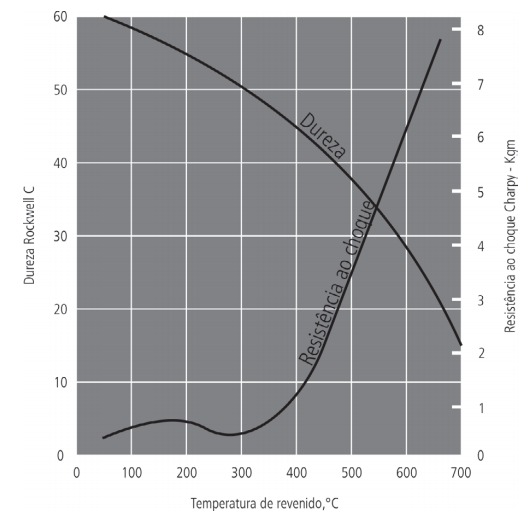
\includegraphics[width=0.75\textwidth]{dureza_resistencia_revenido}
		\caption{Comportamento da dureza e da resistência ao choque (obtida em ensaio Charpy) em função da temperatura de revenimento para um aço 1045 temperado. \cite{vale2016tratamento}}
		\label{fig:dureza_resistencia_revenido}
	\end{figure}
	

\section{Micrografia}
	
	No estudo da ciência dos materiais, usualmente é necessário ou desejável examinar os elementos estruturais e os defeitos que influenciam as propriedades dos materiais. Alguns detalhes estruturais possuem dimensões macroscópicas e podem ser observados a olho nu, porém alguns outros são elementos microscópios de devem ser observados e analisados com o auxílio de equipamentos.
	
	Na maioria dos materiais, os grãos constituintes possuem dimensões microscópicas \citep{callister2011materials}, com diâmetros que podem chegar à ordem de micrômetros. Nesse caso, a observância de sua microestrutura deve ser feita utilizando-se algum tipo de microscópio.
	
	Duas características importantes a se observar na microestrutura de um material são o tamanho e a forma do grão.
	
	Microscópios ópticos e microscópios de varredura por sonda são comumente utilizados em microscopia \cite{callister2011materials}. Esses instrumentos auxiliam nas investigações das características microestruturais de todos os tipos de materiais. 
	
	Aplicações importantes das análises microestruturais são \cite{callister2011materials}:
	\begin{itemize}
		\item Assegurar que as associações entre as propriedades e a estrutura (e os defeitos) sejam compreendidas da forma correta;
		\item Prever as propriedades dos materiais uma vez que essas relações tenham sido estabelecidas;
		\item Projetar ligas com novas combinações de propriedades;
		\item Determinar se um material foi ou não tratado termicamente de maneira correta;
		\item Verificar o modo de uma fratura mecânica.
	\end{itemize}

	Existem duas técnicas de microscopia muito comuns para esse tipo de análise, que são a microscopia óptica e a microscopia eletrônica.


\subsection{Microscopia ótica}
	Na microscopia ótica, o microscópio é utilizado para estudar a microestrutura. É necessária uma preparação cuidadosa da superfície para revelar os detalhes importantes da microestrutura. A amostra deve ser lixada e polida, até atingir um acabamento liso e espelhado. Posteriormente é realizado um ataque químico com um reagente apropriado para revelar a microestrutura. A reatividade química dos grãos com o reagente depende da orientação cristalográfica, assim, as características do ataque químico variam de grão para grão \cite{callister2011materials}.
	
	Com o ataque químico, os diferentes tipos de grãos são revelados. Cada grão torna-se identificável quando visto pelo microscópio, uma vez que reflete a luz em uma angulação própria (Fig. \ref{fig:ataque_grao}), apresentando cada imagem uma característica própria. 
	
	\begin{figure}[H]
		\centering
		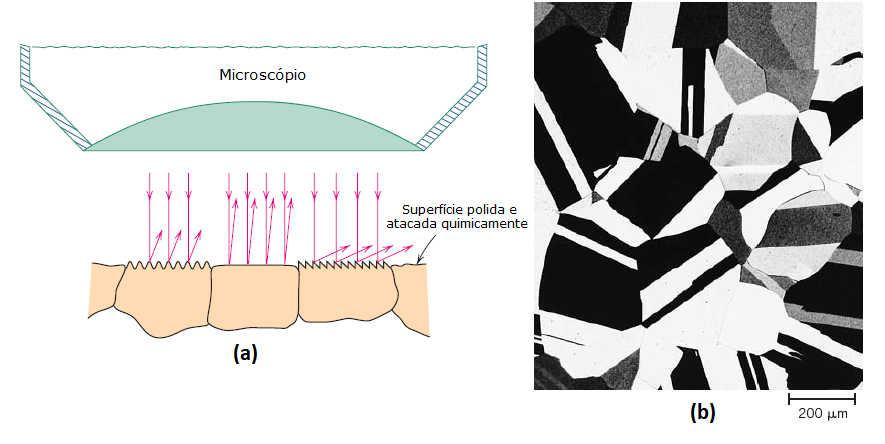
\includegraphics[width=0.90\textwidth]{ataque_grao}
		\caption{a) Reflexão dos raios de luz na superfície do grão atacado quimicamente. b) Fotomicrografia gerada, onde é possível identificar claramente os diferentes grãos. \cite{callister2011materials}}
		\label{fig:ataque_grao}
	\end{figure}

	Também por decorrência do ataque químico são formados sulcos ao longo dos contornos de grão, que também é identificável por conta do tipo de reflexão que a luz sofre nessa região, conforme mostrado na Fig. \ref{fig:ataque_contorno}.
	
	\begin{figure}[H]
		\centering
		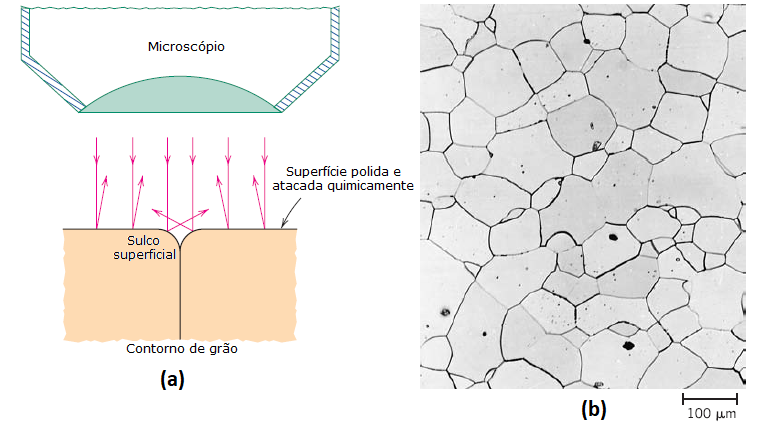
\includegraphics[width=0.9\textwidth]{ataque_contorno}
		\caption{a) Reflexão dos raios de luz no sulco entre os grãos atacados quimicamente. b) Fotomicrografia gerada, onde é possível identificar as regiões de contornos de grão mais escuras. \cite{callister2011materials}}
		\label{fig:ataque_contorno}
	\end{figure}

	Para a análise de uma microestrutura de uma liga bifásica, é selecionado um reagente químico que seja capaz de produzir uma textura diferente para cada fase (ou cada grão). Dessa forma, as diferentes fases podem ser distinguidas entre si.
	
\subsection{Microscopia eletrônica}
	A microscopia eletrônica é utilizada para a observação de detalhes muito finos ou pequenos, que não podem ser observados pelo microscópio óptico, que possui ampliação máxima possível de aproximadamente 2000 vezes \cite{callister2011materials}. O microscópio eletrônico tem a capacidade de ampliação muito maior e pode ser empregado nesses casos.
	
	Na tecnologia de microscopia eletrônica, a estrutura que está sendo investigada é formada utilizando feixes de elétrons no lugar de radiação luminosa, como é no caso da microscopia óptica. 
	De acordo com a mecânica quântica, um elétron a alta velocidade terá características ondulatórias, possuindo um comprimento de onda inversamente proporcional a sua velocidade \cite{callister2011materials}. O feixe de elétrons é direcionado contra a superfície a ser analisada e sua imagem é formada por lentes magnéticas, que captam o comportamento do elétron ao interagir com a superfície do material.
	
	A microscopia eletrônica de varredura (MEV) é uma técnica muito útil dentro dos tipos de microscopia eletrônica. Nessa tecnologia, o material a ser analisado é varrido por um feixe de elétrons, que é refletido, captado e exibido sobre um tubo de raios catódicos. Essa imagem exibida pode, então, ser fotografada e representa as características da superfície analisadas. A superfície a ser analisada no MEV pode ou não estar polida e atacada quimicamente, porém esta deve ser condutora de eletricidade \cite{callister2011materials}. Na microscopia eletrônica de varredura são possíveis ampliações de 10 a até mais de 50 000 vezes.


\section{Dureza dos materiais} 

	Existem dois tipos de medições de dureza comumente aplicadas para determinar a dureza de um material qualquer: por risco e por penetração.

\subsection{Dureza por risco}

	A dureza por risco pode ser avaliada a partir da capacidade de um material riscar outro elemento
	A escala de dureza Mohs se consiste de dez minerais organizados em ordem crescente de dureza, sendo que cada mineral pode riscar o mineral na posição na escala abaixo, mas não pode riscar o material na escala acima \cite{tabor1953mohs}. A tabela é organizada na escala de 1 a 10, sendo o talco o material mais macio e o diamante o mais duro. A escala Mohs está representada na Tab. \ref{tab:mohs}

	\begin{table}[H]
	\centering
	\caption{Escala Mohs para os elementos.}
	\begin{tabular}{|c|c|}
		\hline
		\textbf{Escala} & \textbf{Elemento} \bigstrut\\
		\hline
		1          & Talco \bigstrut\\
		\hline
		2          & Gesso \bigstrut\\
		\hline
		3          & Calcite \bigstrut\\
		\hline
		4          & Fluorite \bigstrut\\
		\hline
		5          & Apatite \bigstrut\\
		\hline
		6          & Ortose \bigstrut\\
		\hline
		7          & Quartzo \bigstrut\\
		\hline
		8          & Topázio \bigstrut\\
		\hline
		9          & Corindo \bigstrut\\
		\hline
		10         & Diamante \bigstrut\\
		\hline
	\end{tabular}%
	\label{tab:mohs}%
	\end{table}%

	A dureza por risco é a propriedade característica de um material sólido, que expressa sua resistência a deformações permanentes e está diretamente relacionada com a força de ligação dos átomos.

\subsection{Dureza por penetração}

	A dureza por penetração é outra maneira de avaliar a dureza, através da capacidade de um material penetrar o outro. Experimentos mostram que durante a penetração e durante o deslizamento o comportamento dos materiais é determinado pelas propriedades plásticas dos materiais. Isso sugere a existência de uma relação entre a escala Mohs para dureza (por risco) e a dureza por penetração \cite{tabor1953mohs}.

	Na engenharia e na metalurgia, sua determinação se dá através do ensaio de penetração, que mede da dureza do material. Para cada tipo de material, faz-se necessário um tipo de teste mais apropriado, surgindo então diversas unidades de dureza com diferentes escalas, alguns exemplos são as escalas Rockwell, Brinell e Vickers.

	Para o teste de dureza Rockwell, faz-se necessário a utilização do durômetro (Fig. \ref{fig:durometro}). O funcionamento do durômetro se baseia na profundidade de penetração de um penetrador sobre uma peça a se analisar. O valor indicado na escala do mostrador do durômetro é o valor da dureza, que corresponde a profundidade alcançada pelo penetrador.
	

	\begin{figure}[H]
		\centering
		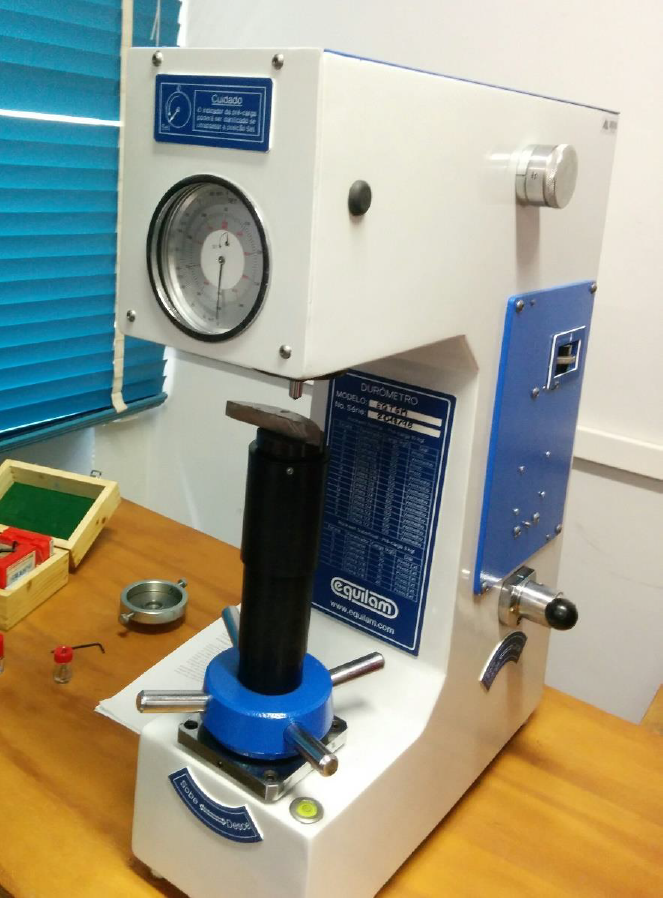
\includegraphics[width=0.5\textwidth]{durometro}
		\caption{Durômetro.}
		\label{fig:durometro}
	\end{figure}

	Duas cargas são exercidas impostas durante o teste de dureza. A primeira é a pré-carga, que tem como objetivo penetrar o material até uma profundidade em que não mais haja a recuperação plástica após a retirada da carga sobre o material. Após a pré-carga, será exercida a carga maior, conforme a Fig. \ref{fig:dureza_rockwell}. A carga maior é aplicada lentamente enquanto o durômetro mede a profundidade de penetração, ou dureza.

	\begin{figure}[H]
		\centering
		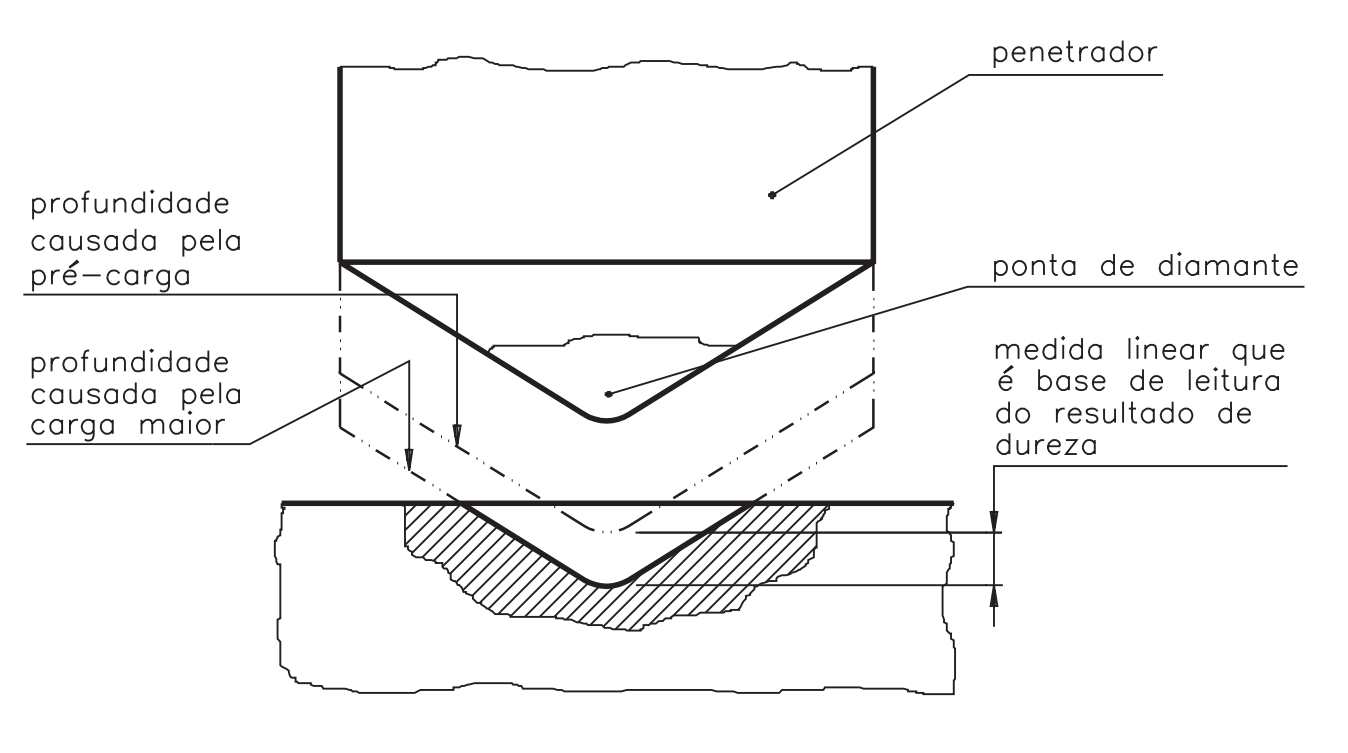
\includegraphics[width=0.8\textwidth]{dureza_rockwell}
		\caption{Esquema de penetração com a pré-carga e a carga maior. \cite{esselrockwell}}
		\label{fig:dureza_rockwell}
	\end{figure}

	O método Rockwell é um método de medição direta da dureza, sendo um dos mais utilizados em indústrias. Esse é um dos métodos mais simples e que não requer habilidades especiais do operador. Além disso, várias escalas diferentes (Ex.: Rockwell A, B, C) podem ser utilizadas através de possíveis combinações de diferentes penetradores e cargas, o que permite o uso desse ensaio em praticamente todas as ligas metálicas, assim como em muitos polímeros.
	
	A escala Rockwell C é adequada para diversas gamas de aços, inclusive os de composição eutetóide. Na escala Rockwell C, é utilizado um penetrador com ponta cônica de diamante, uma carga maior de 150 kgf e uma pré-carga padrão de 10 kgf. A Figura \ref{fig:teste_dureza} mostra a execução de um teste de dureza de um aço qualquer.
	
	\begin{figure}[H]
		\centering
		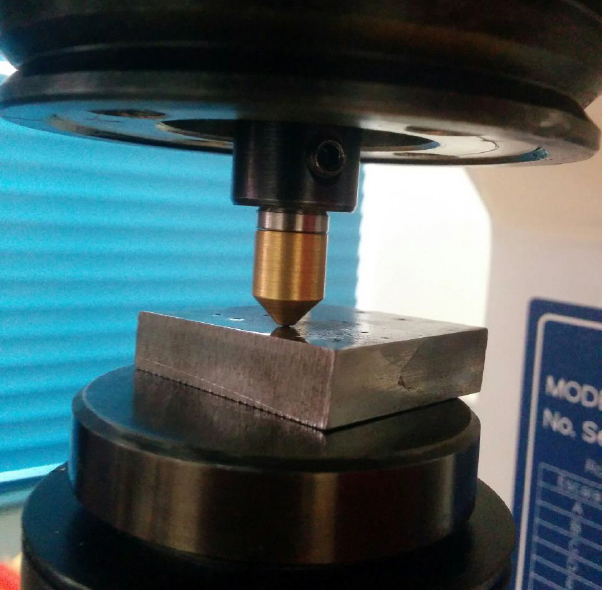
\includegraphics[width=0.4\textwidth]{teste_dureza}
		\caption{Teste de dureza de um aço.}
		\label{fig:teste_dureza}
	\end{figure}

\pagebreak	


	
	
		
	
		
\chapter{METODOLOGIA}
	
\section{O Experimento}

	O procedimento consiste em testar duas amostras perlíticas e duas bainíticas em um tribômetro. As amostras foram usinadas a partir do material de uma roda ferroviária forjada real, de composição de um aço próximo ao eutetóide. Cada amostra foi analisada três vezes seguidas para uma carga fixa exercida por uma massa padronizada de 5 kg, conforme a Fig. \ref{fig:esquema_teste}.

	\begin{figure}[H]
		\centering
		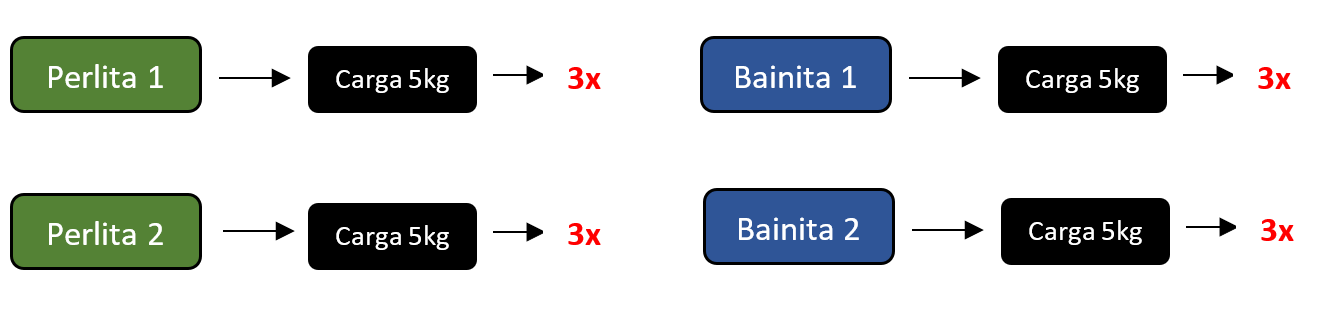
\includegraphics[width=1\textwidth]{esquema_teste}
		\caption{Esquema de procedimento de testes para cada amostra perlítica e bainítica.}
		\label{fig:esquema_teste}
	\end{figure}

	Cada teste é conduzido por 1 hora no tribômetro do tipo rolo contra disco a fim de se analisar a perda de massa da amostra durante este intervalo de tempo. Ao final de todos os testes, os resultados de desgaste por perda de massa de cada amostra serão comparados e analisados entre si.
	
	O tribômetro da Universidade Federal de Juiz de Fora (UFJF) é do tipo rolo contra disco. Nesse tipo de tribômetro, o rolo (ou corpo) é do mesmo material da roda ferroviária e corre sobre o disco (ou contracorpo), que é do mesmo material do trilho. Uma foto do tribômetro utilizado neste estudo é mostrada na Fig. \ref{fig:tribometro}.
	
	\begin{figure}[H]
		\centering
		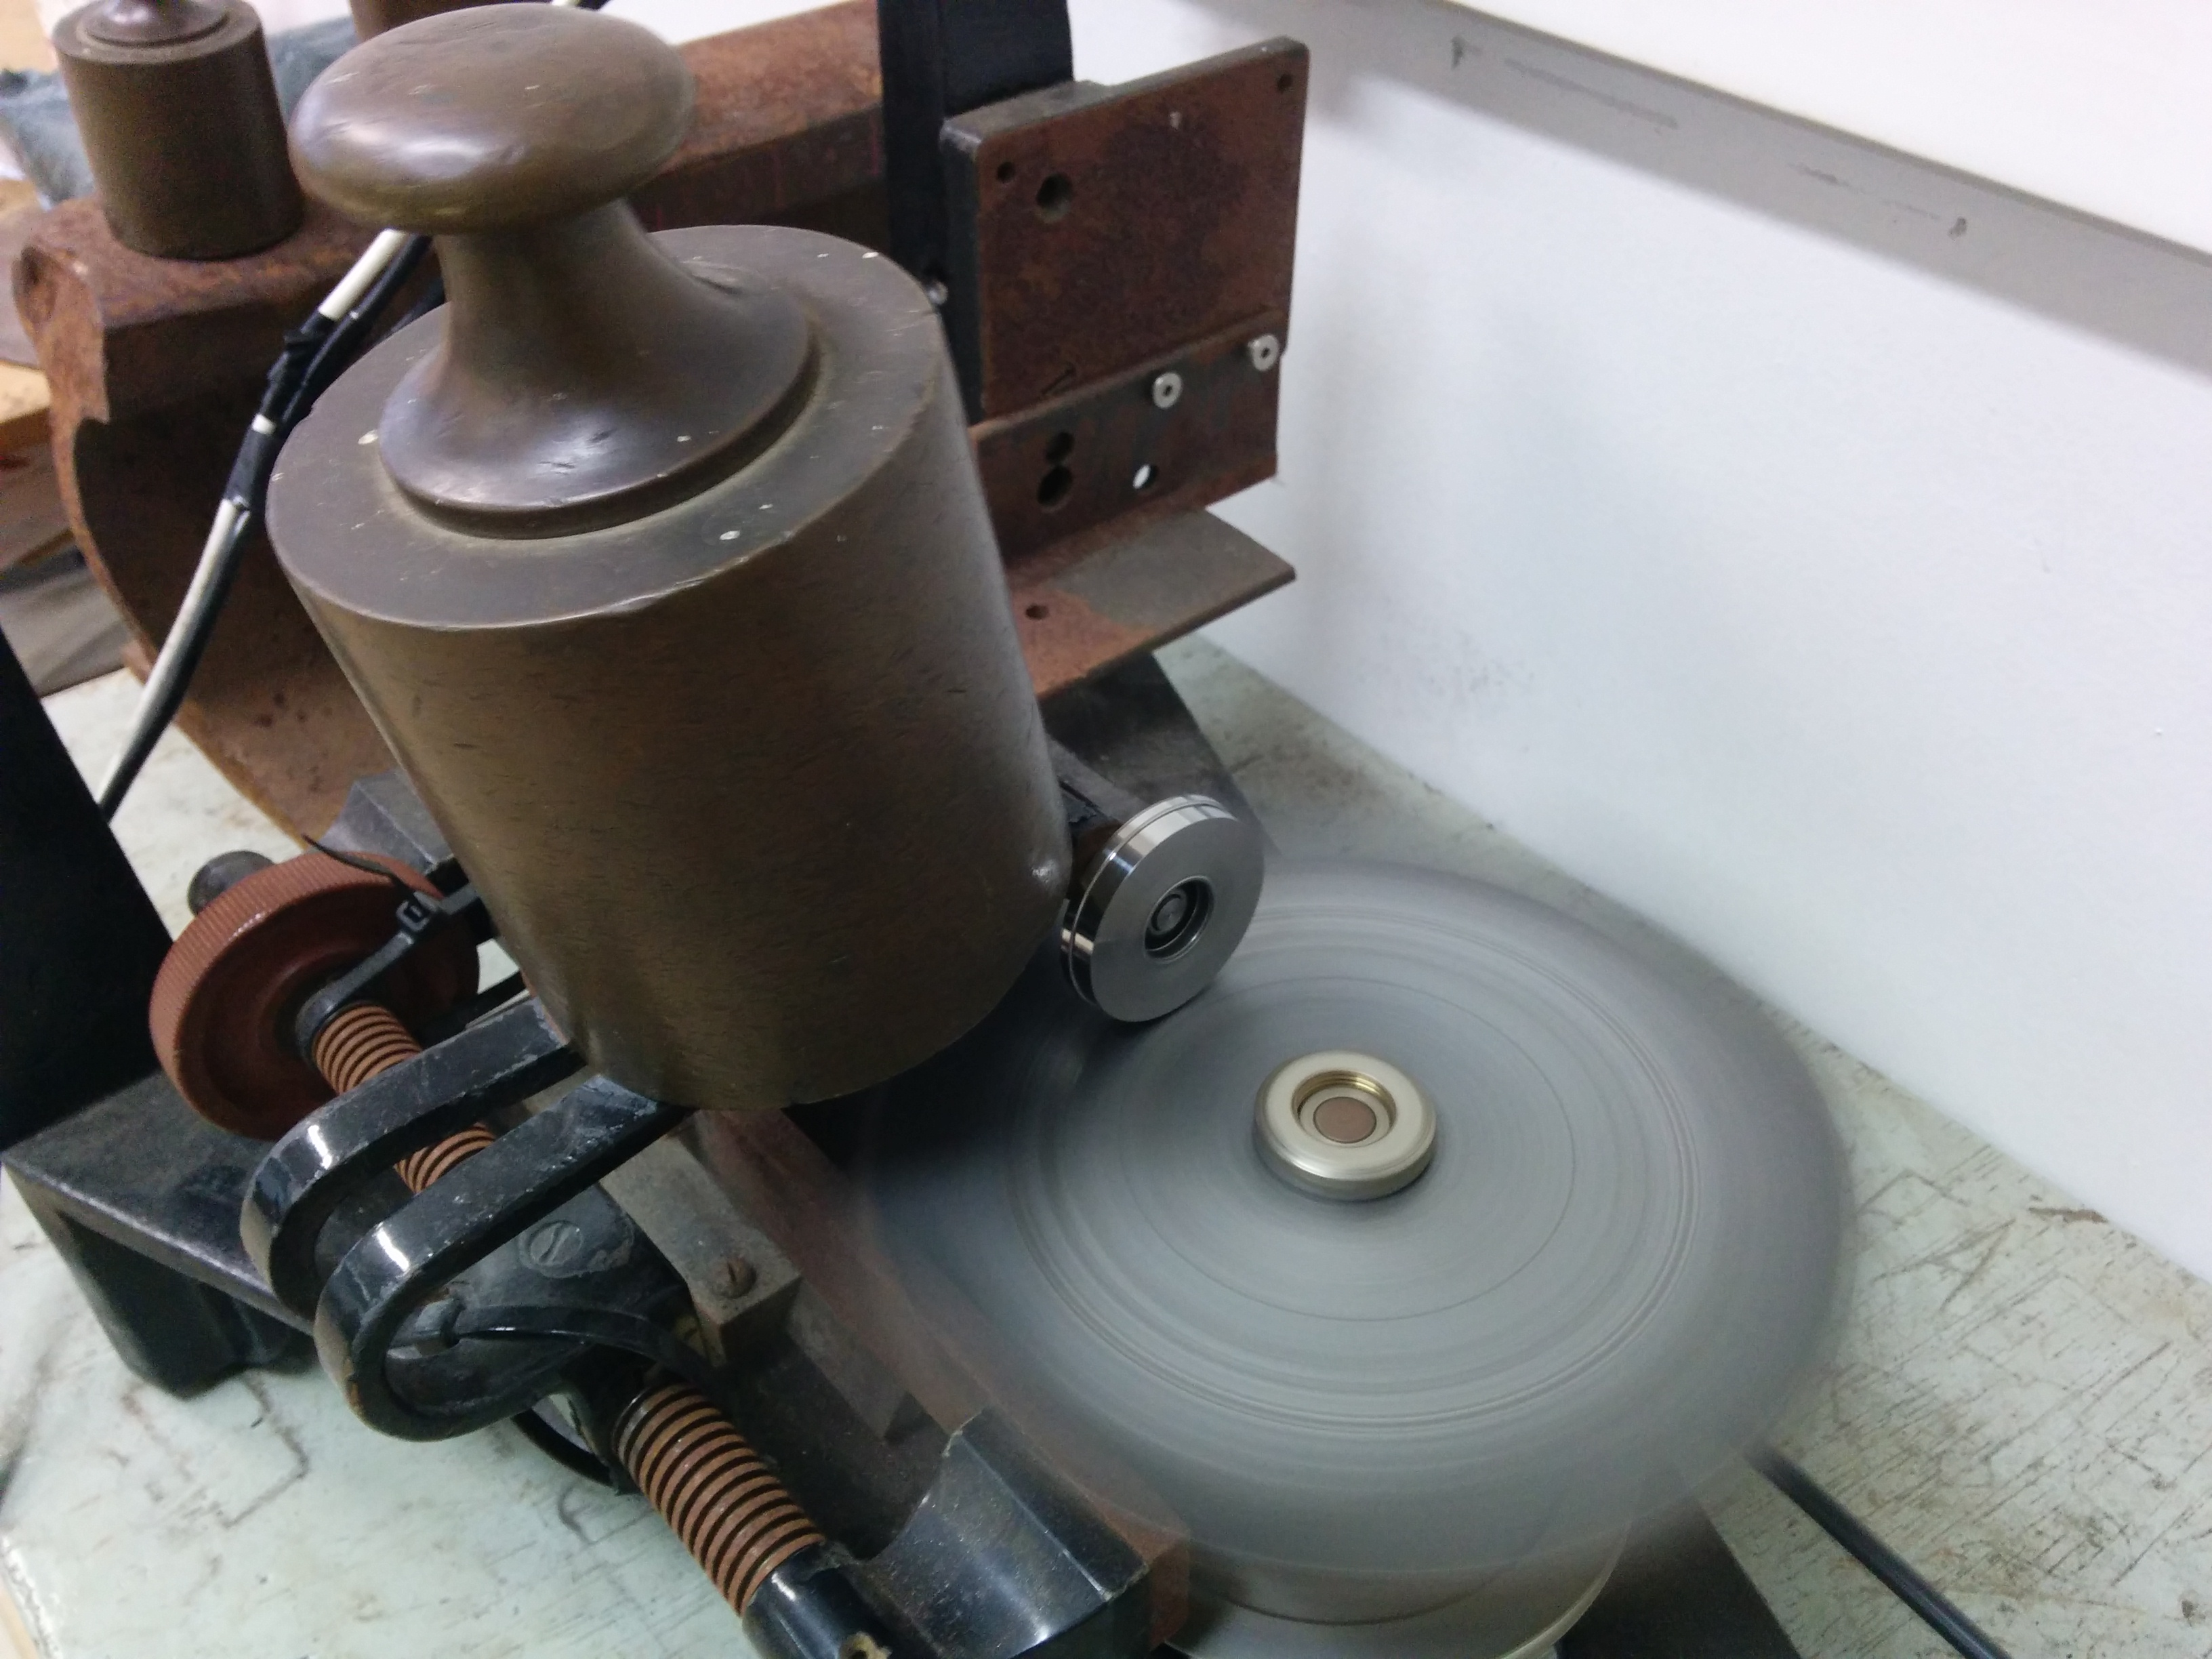
\includegraphics[width=0.75\textwidth]{tribometro}
		\caption{Tribômetro do tipo rolo contra disco utilizado nos ensaios.}
		\label{fig:tribometro}
	\end{figure}

	Em seu funcionamento, o disco, do mesmo material do trilho, gira com rotação constante. A amostra de roda a ser testada é encaixada em um eixo conectado a um braço, que tem liberdade de rotação. Assim, ao se apoiar uma carga sobre o pino, uma força normal (ou carga) é exercida na roda sobre o disco, simulando o rolamento de um trem sobre a linha férrea. Seu esquema de funcionamento está ilustrado na Fig. \ref{fig:esquema_tribometro}.
	
	\begin{figure}[H]
		\centering
		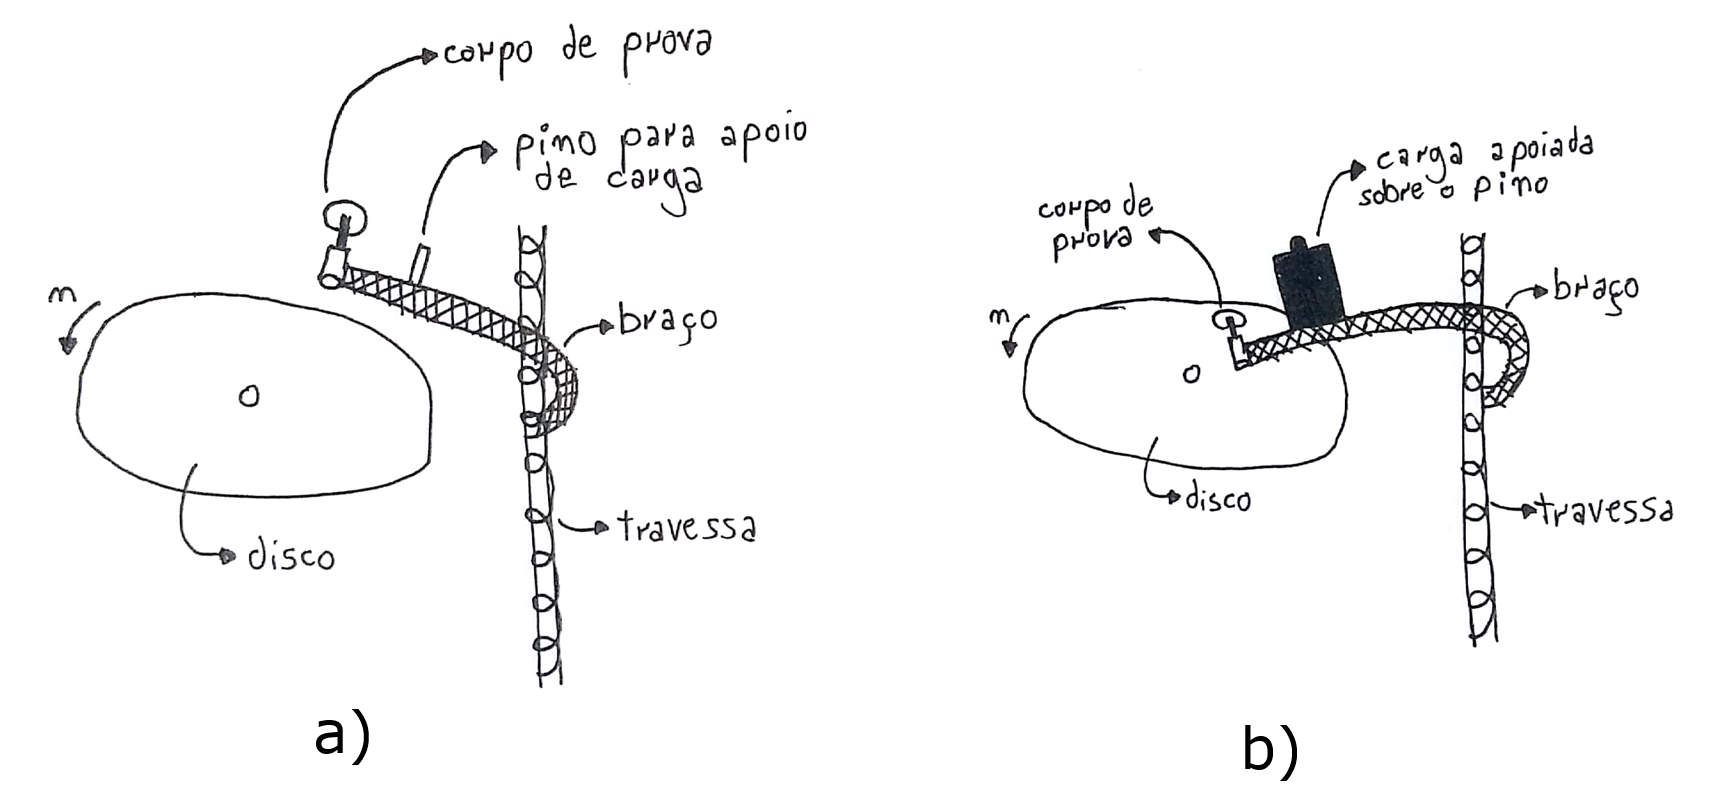
\includegraphics[width=1\textwidth]{esquema_tribometro}
		\caption{Esquema de funcionamento do tribômetro desenvolvido nos laboratórios na UFJF. Em (a), o corpo de prova está livre de carga e não exerce força sobre o disco. Em (b), é colocada uma carga sobre o pino de apoio carga, que desloca o braço no sentido transversal e força o corpo de prova sobre o disco.}
		\label{fig:esquema_tribometro}
	\end{figure}
	
	Os ensaios foram realizados no Laboratório de Processos de Fabricação, Laboratório de Metalografia e Mecânica da Faculdade de Engenharia e no Laboratório de Química da Universidade Federal de Juiz de Fora.
	
\section{Preparação das amostras}

	As amostras ensaiadas foram retiradas de uma roda forjada fabricada em aço de composição próxima à eutetóide. A Figura \ref{fig:secao_roda} mostra esquematicamente o local de retirada das amostras.
	
	O material para a posterior usinagem das amostras foi retirado a aproximadamente 10 mm da superfície da pista de rolamento, conforme mostrado na Fig. \ref{fig:secao_roda}. O bloco retirado é de aproximadamente 15 mm de espessura, 100 mm de largura e 140 mm de comprimento. Esse local de retirada foi estrategicamente escolhido uma vez que, tipicamente, esta região da roda é constituída predominantemente por perlita fina.
	
	\begin{figure}[H]
		\centering
		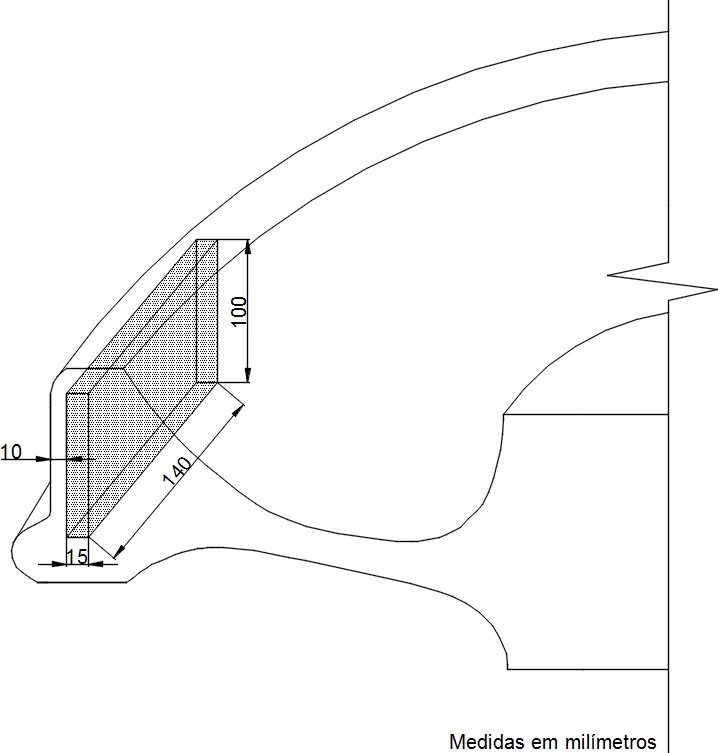
\includegraphics[width=0.5\textwidth]{secao_roda}
		\caption{Desenho esquemático de um quarto de uma roda ferroviária real, destacando-se o local de retirada do material das amostras. \cite{paula2016desgaste}}
		\label{fig:secao_roda}
	\end{figure}

	Os cortes do bloco a partir da roda original foram realizados com o auxílio de uma serra de fita. Todos os cortes foram realizados com lubrificação, com o devido cuidado para que não ocorresse superaquecimento e consequentemente transformação microestrutural do aço.

	Desse bloco retirado de uma roda real, são preparadas 6 amostras em formato de roda. As rodas em miniatura preparadas têm as dimensões de 8 mm de espessura, \linebreak 39 mm de diâmetro externo e 15 mm de diâmetro interno, onde será acoplado um rolamento. Na superfície de rolamento da amostra foi feito um chanfro de forma que a espessura do contato seja de 2 mm apenas, aumentando, assim, a pressão do contato roda-trilho. A Figura \ref{fig:amostra_roda_pura} mostra o formato da roda usinada a partir do material bruto.
	
	\begin{figure}[H]
		\centering
		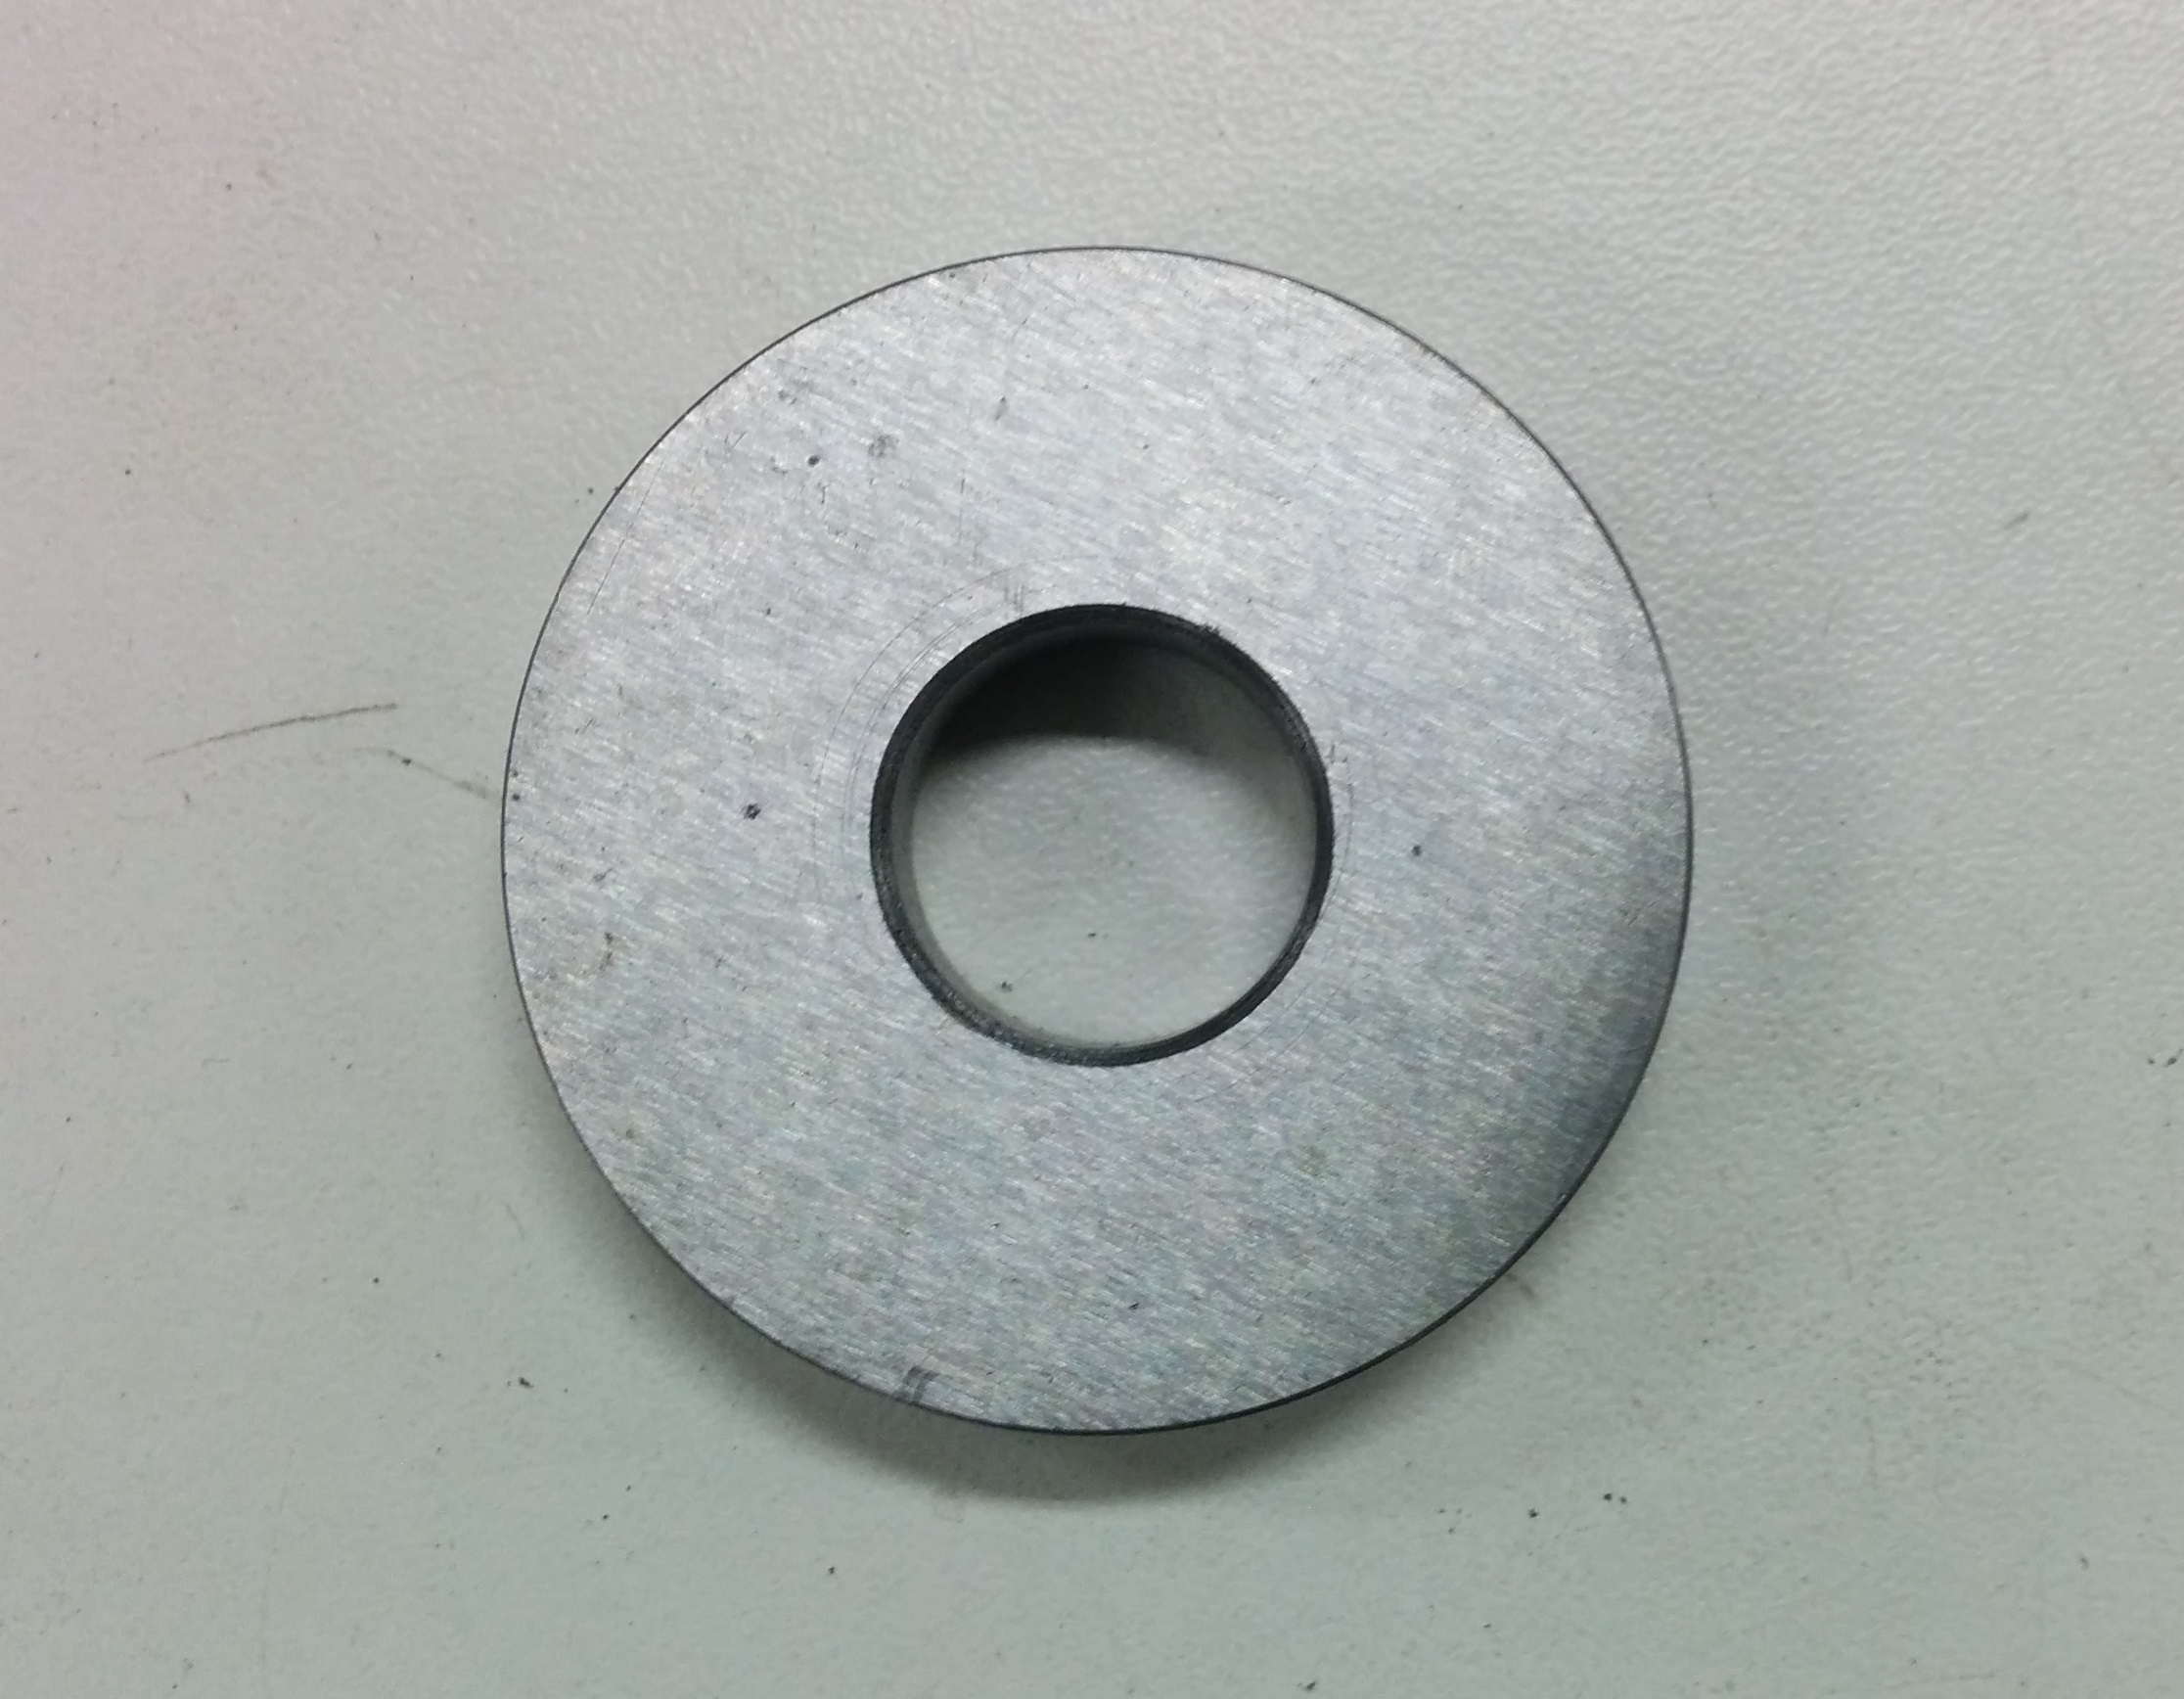
\includegraphics[width=0.55\textwidth]{amostra_roda_pura}
		\caption{Roda em miniatura usinada a partir do material retirado da roda real.}
		\label{fig:amostra_roda_pura}
	\end{figure}
	
	Das 6 rodas, 3 serão utilizadas como amostras perlíticas, já que a região de retirada já é composta predominantemente por perlita fina. As outras 3 rodas serão tratadas termicamente a fim de se obter a microestrutura bainítica. De cada grupo das 3 amostras, 2 serão utilizadas para teste, enquanto a última será cortada para se realizar uma micrografia e analisar sua microestrutura interna. O esquema de utilização de cada amostra está representado na Fig. \ref{fig:amostras}.
	
	\begin{figure}[H]
		\centering
		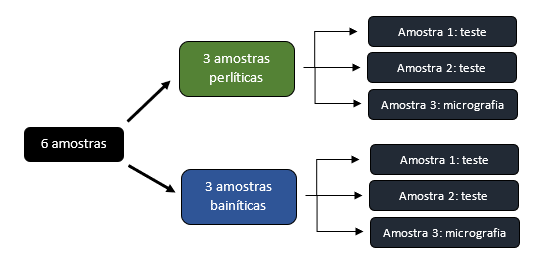
\includegraphics[width=1\textwidth]{amostras}
		\caption{Esquema de utilização de cada amostra.}
		\label{fig:amostras}
	\end{figure}

	Foi realizada também uma espectrometria do material das amostras, a fim de se obter uma análise quantitativa detalhada da composição química do aço. O resultado está representado na Tab. \ref{tab:composicao}.
	
	\begin{table}[H]
	\centering
	\caption{Composição química das amostras via Espectrômetro de Emissão Óptica}
	\resizebox{0.45\textwidth}{!}{%
	\begin{tabular}{|p{8em}|c|}
		\hline
		\textbf{Elementos} & \multicolumn{1}{p{8em}|}{\textbf{Identificação das Amostras}} \bigstrut\\
		\hline
		Carbono (\%) & 0,760 \bigstrut\\
		\hline
		Manganês (\%) & 0,846 \bigstrut\\
		\hline
		Silício (\%) & 0,906 \bigstrut\\
		\hline
		Fósforo(\%) & 0,014 \bigstrut\\
		\hline
		Enxofre(\%) & 0,017 \bigstrut\\
		\hline
		Cromo (\%) & 0,096 \bigstrut\\
		\hline
		Molibdênio (\%) & 0,032 \bigstrut\\
		\hline
		Níquel (\%) & 0,022 \bigstrut\\
		\hline
		Alumínio (\%) & 0,004 \bigstrut\\
		\hline
		Cobre (\%) & 0,034 \bigstrut\\
		\hline
		Boro (\%)  & 0,000 \bigstrut\\
		\hline
		Vanádio (\%) & 0,002 \bigstrut\\
		\hline
		Cobalto (\%) & 0,007 \bigstrut\\
		\hline
	\end{tabular}%
	}
	\label{tab:composicao}%
	\end{table}%


\subsection{Roda perlítica}
	Como o material das amostras foi retirado à 10 mm da superfície da pista de rolamento, não foi necessário posteriores tratamentos do aço, já que, no local de retirada do material desta roda em específico, a microestrutura predominantemente é a própria perlita fina.
	
	Um rolamento do tipo 696RS, com 15 mm de diâmetro externo e 6 mm de diâmetro interno, foi acoplado à roda. A montagem final da amostra com o rolamento é mostrada na Fig. \ref{fig:amostra_perlita}.
	
	\begin{figure}[H]
		\centering
		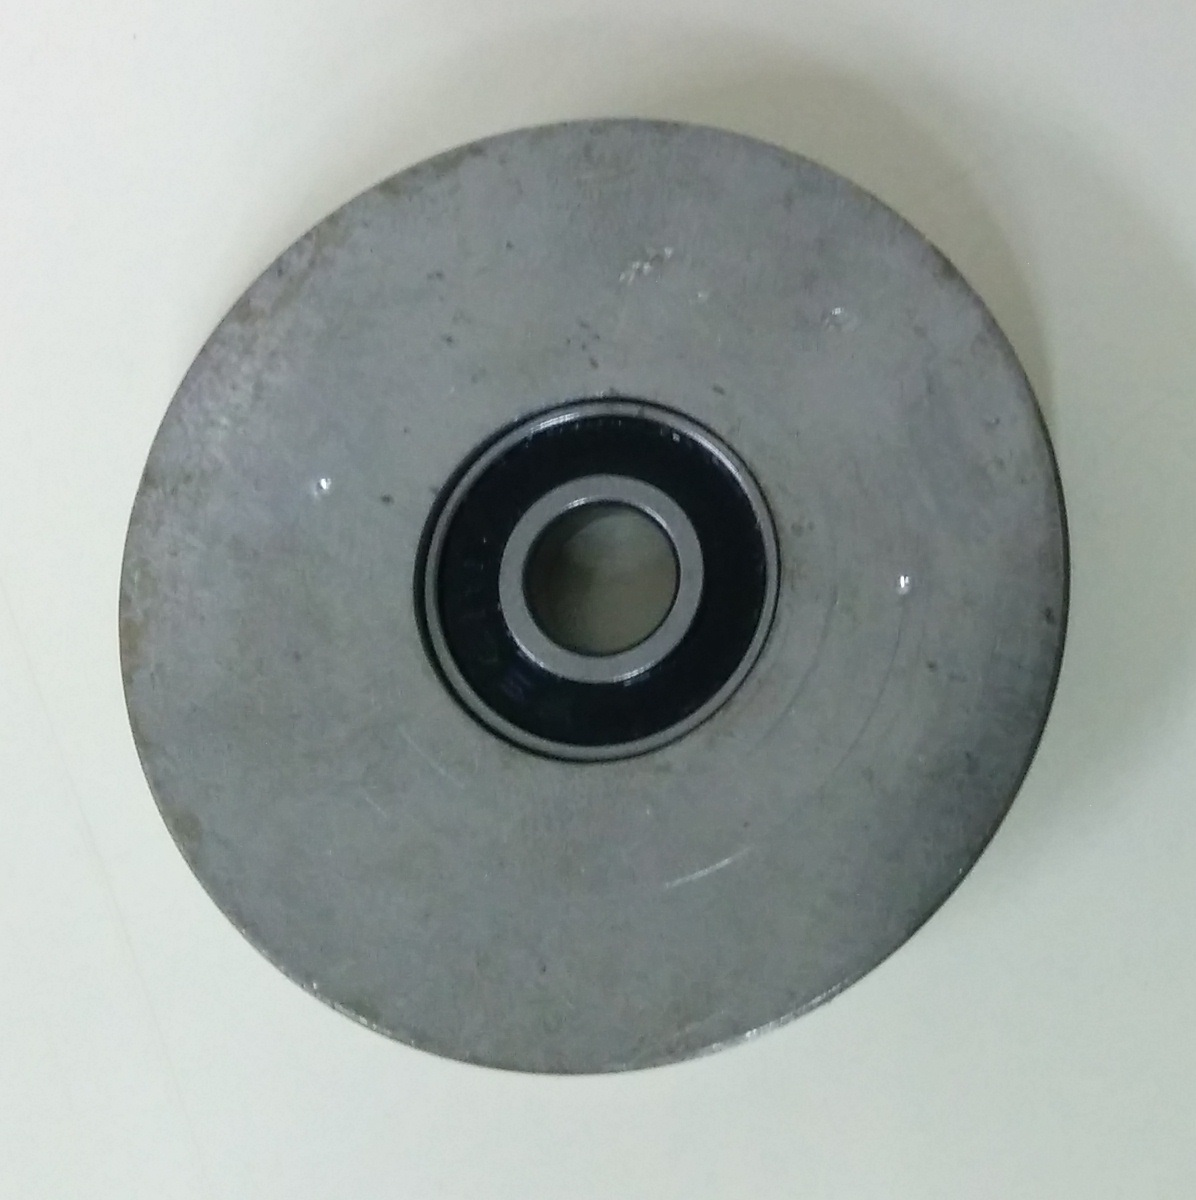
\includegraphics[width=0.5\textwidth]{amostra_perlita}
		\caption{Amostra perlítica com rolamento.}
		\label{fig:amostra_perlita}
	\end{figure}
	

\subsection{Roda bainítica}

	Para transformar as 3 amostras em microestrutura bainítica, é necessário um realizar um tratamento térmico denominado austêmpera.
	
	Segundo a ASM International, a austêmpera é a transformação isotérmica de uma liga metálica de ferro a uma temperatura abaixo da formação de perlita e acima da formação de martensita \cite{asm1991heat}.
	
	O tratamento de austêmpera em aços oferece a potencial vantagem do aumento da ductilidade, tenacidade e resistência do aço para uma dada dureza \cite{asm1991heat}.
	
	O aço é austemperado através dos seguintes passos:
	\begin{itemize}
		\item Aquecer o material até a temperatura de austenitização, geralmente entre 790$^{\circ}$C e 915$^{\circ}$C;
		\item Mergulhar em um banho em temperatura constante, geralmente entre 260$^{\circ}$C e 400$^{\circ}$C;
		\item Manter sob tal temperatura até que o material sofra transformação isotérmica no banho;
		\item Resfriar sob temperatura ambiente.
	\end{itemize}

	Para a correta austêmpera, o metal deve ser resfriado a partir da temperatura de austenitização para a temperatura do banho rápido o suficiente para que não ocorra transformação da austenita durante o resfriamento. E também o banho deve ser mantido por tempo suficiente para que se tenha certeza de que houve a completa transformação da austenita para a bainita \cite{asm1991heat}.
	
	O tratamento térmico realizado foi feito observando-se a curva de transformação isotérmica (TTT) de um aço eutetóide (Fig. \ref{fig:austempera}).
	
	\begin{figure}[H]
		\centering
		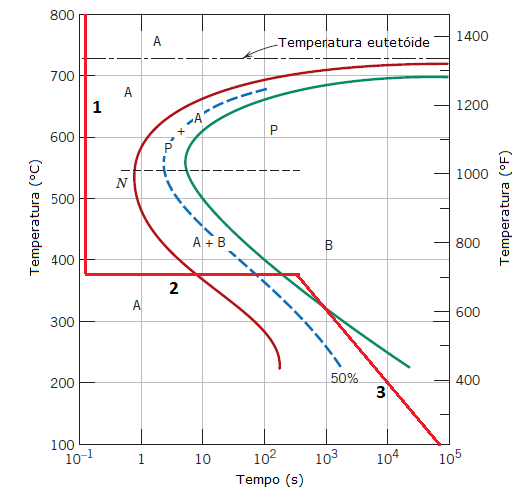
\includegraphics[width=0.8\textwidth]{austempera}
		\caption{Diagrama TTT do aço eutetóide adaptado com linhas representando os passos do tratamento térmico. \cite{callister2011materials} (Adaptado)}
		\label{fig:austempera}
	\end{figure}
	
	A Figura \ref{fig:austempera} mostra o esquema de tratamento térmico feito com base no diagrama TTT do aço eutetóide. Na Figura \ref{fig:austempera}, a linha (1) representa o resfriamento no banho de sais a partir da temperatura de austenitização à 900$^{\circ}$C, a linha (2), a manutenção da temperatura do banho de 380$^{\circ}$C por 5 min e a linha (3), o resfriamento à temperatura ambiente.
	
	A austêmpera realizada neste estudo foi feita no banho de sais (Fig. \ref{fig:sais}), especificamente na mistura de nitrato de potássio e nitrito de sódio. Neste tipo de resfriamento, há uma rápida transferência de calor e também se elimina o problema da barreira de vapor ao redor do material durante o período inicial do banho \cite{asm1991heat}, que prejudica a transferência de calor e, consequentemente, o rápido resfriamento.
	
	\begin{figure}[H]
		\centering
		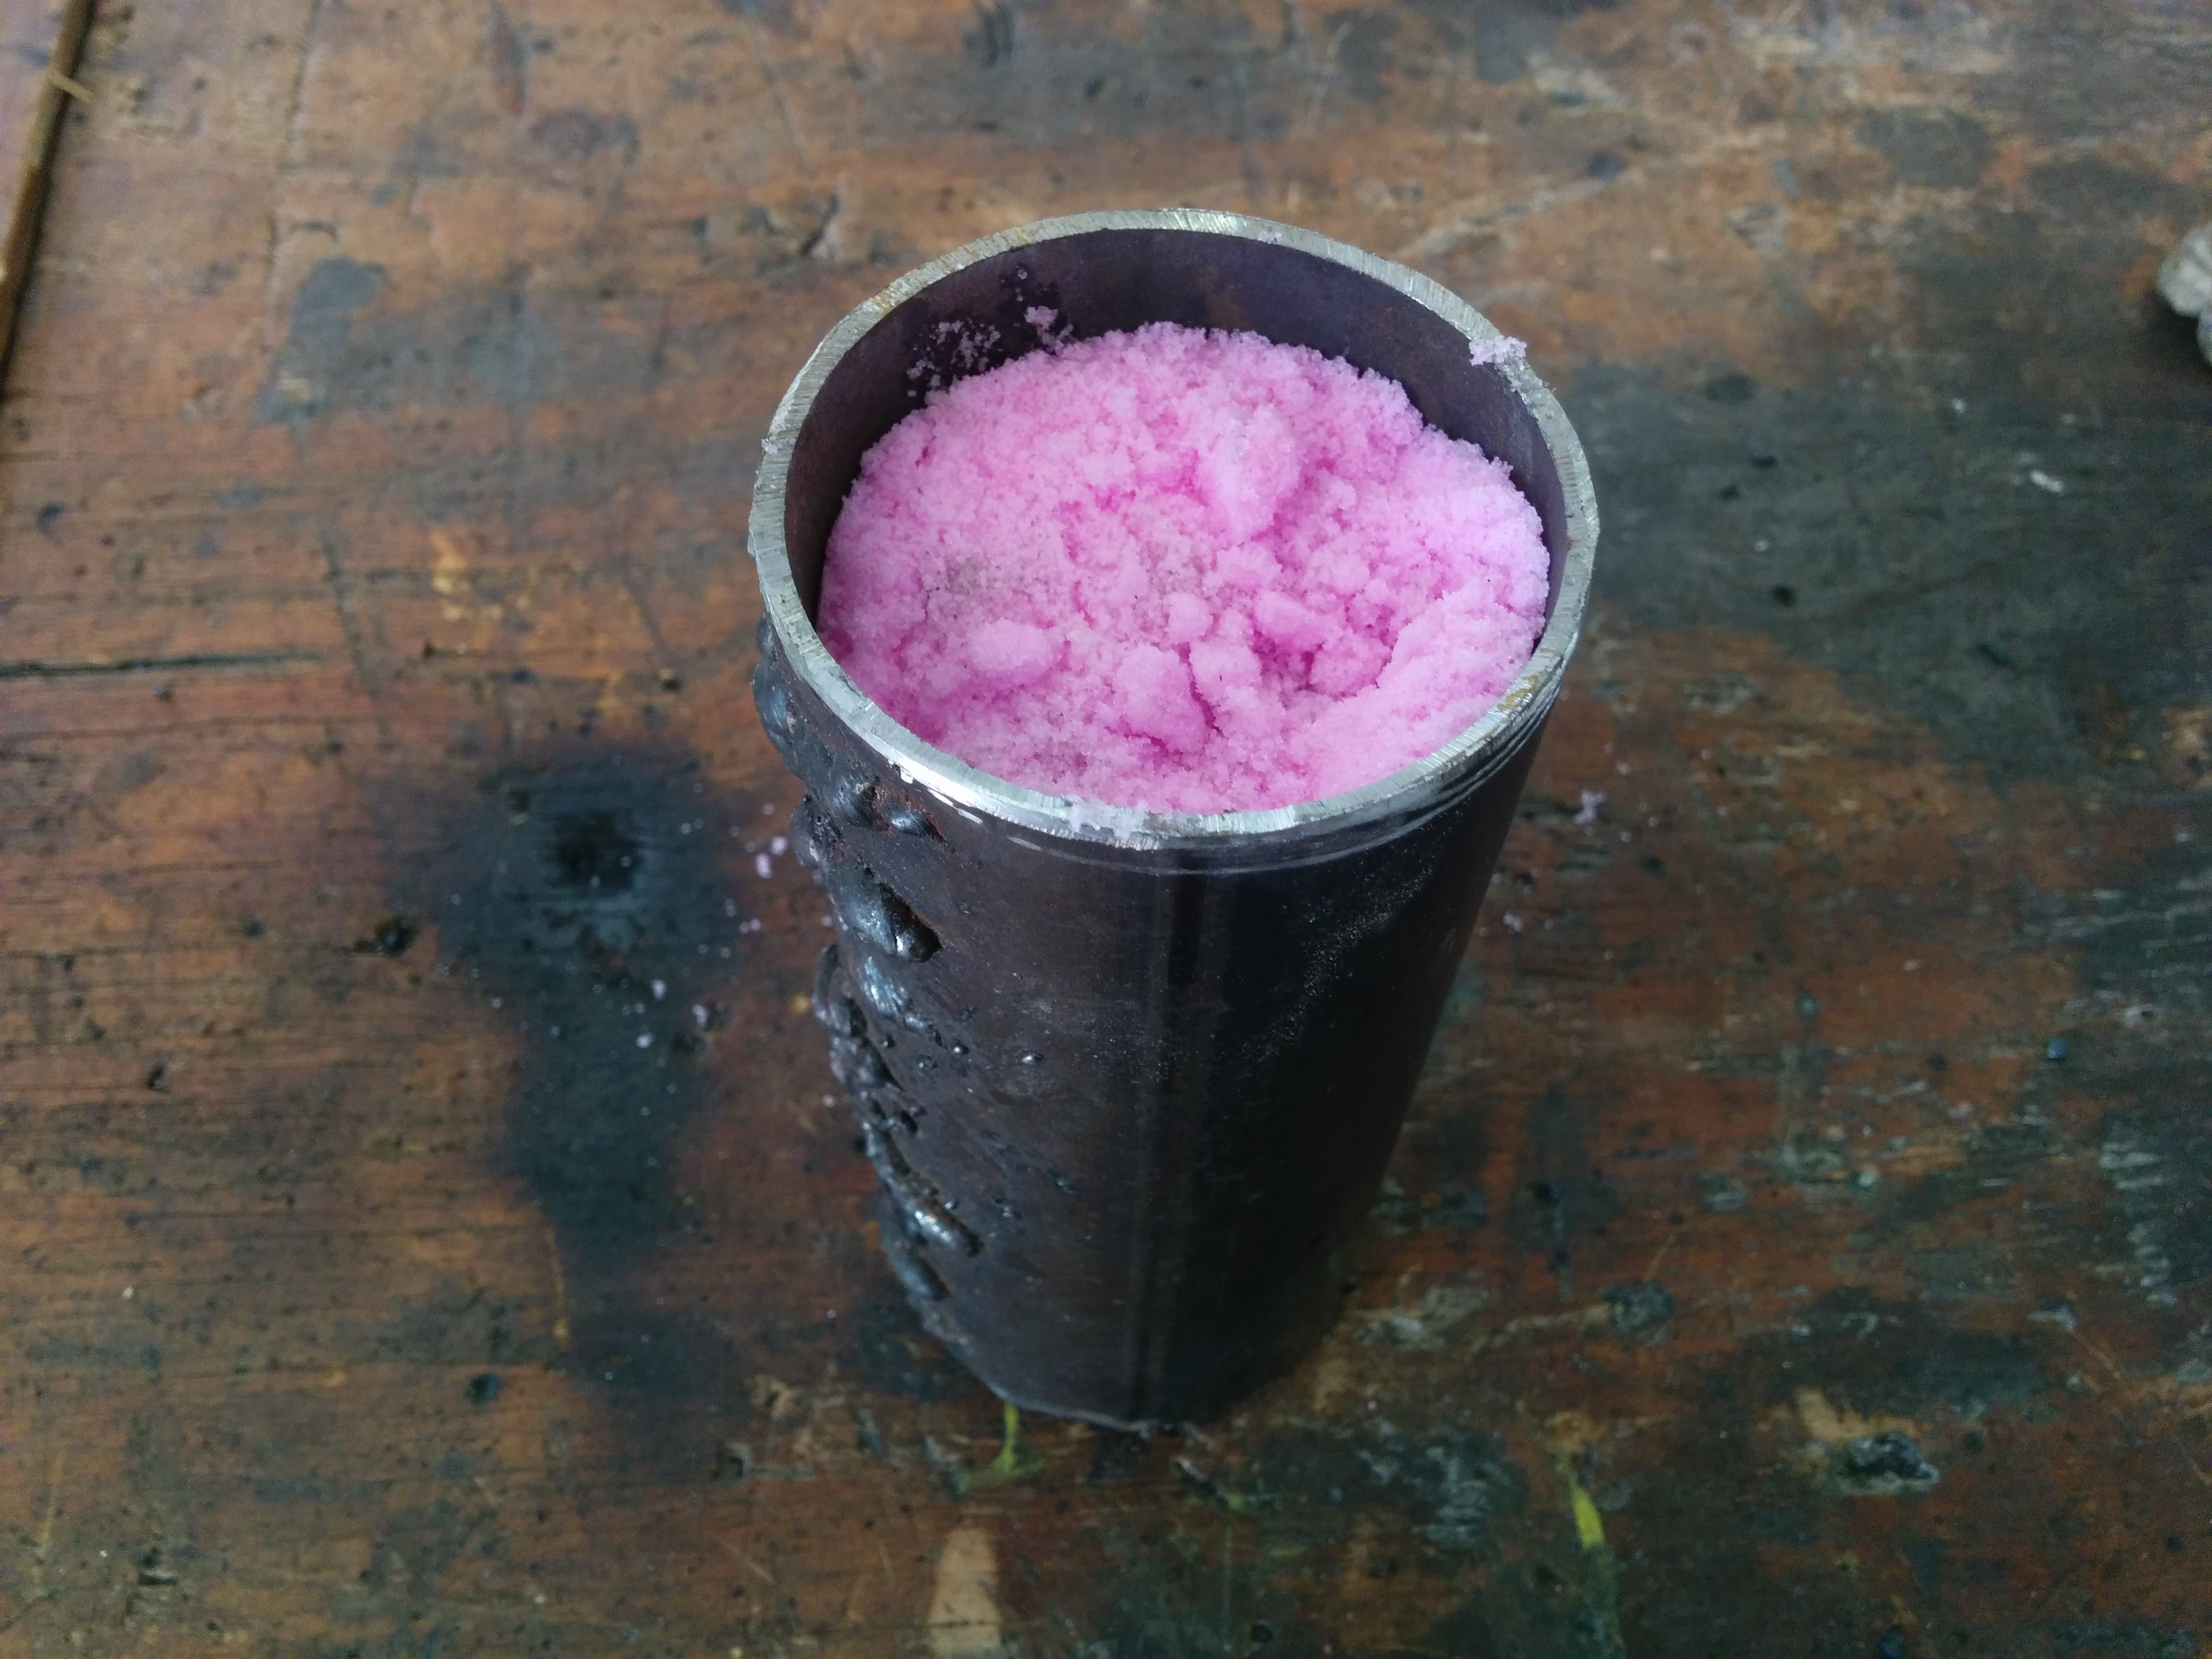
\includegraphics[width=0.7\textwidth]{sais}
		\caption{Recipiente soldado com sal da mistura de nitrato de potássio e nitrito de sódio à temperatura ambiente.}
		\label{fig:sais}
	\end{figure}

	Os sais foram aquecidos no forno até a temperatura de 380$^{\circ}$C (Fig. \ref{fig:forno}), enquanto os corpos de provas se aqueceram na mufla por 15 min à temperatura de 900$^{\circ}$C (Fig. \ref{fig:mufla}).
	
	\begin{figure}[H]
		\centering
		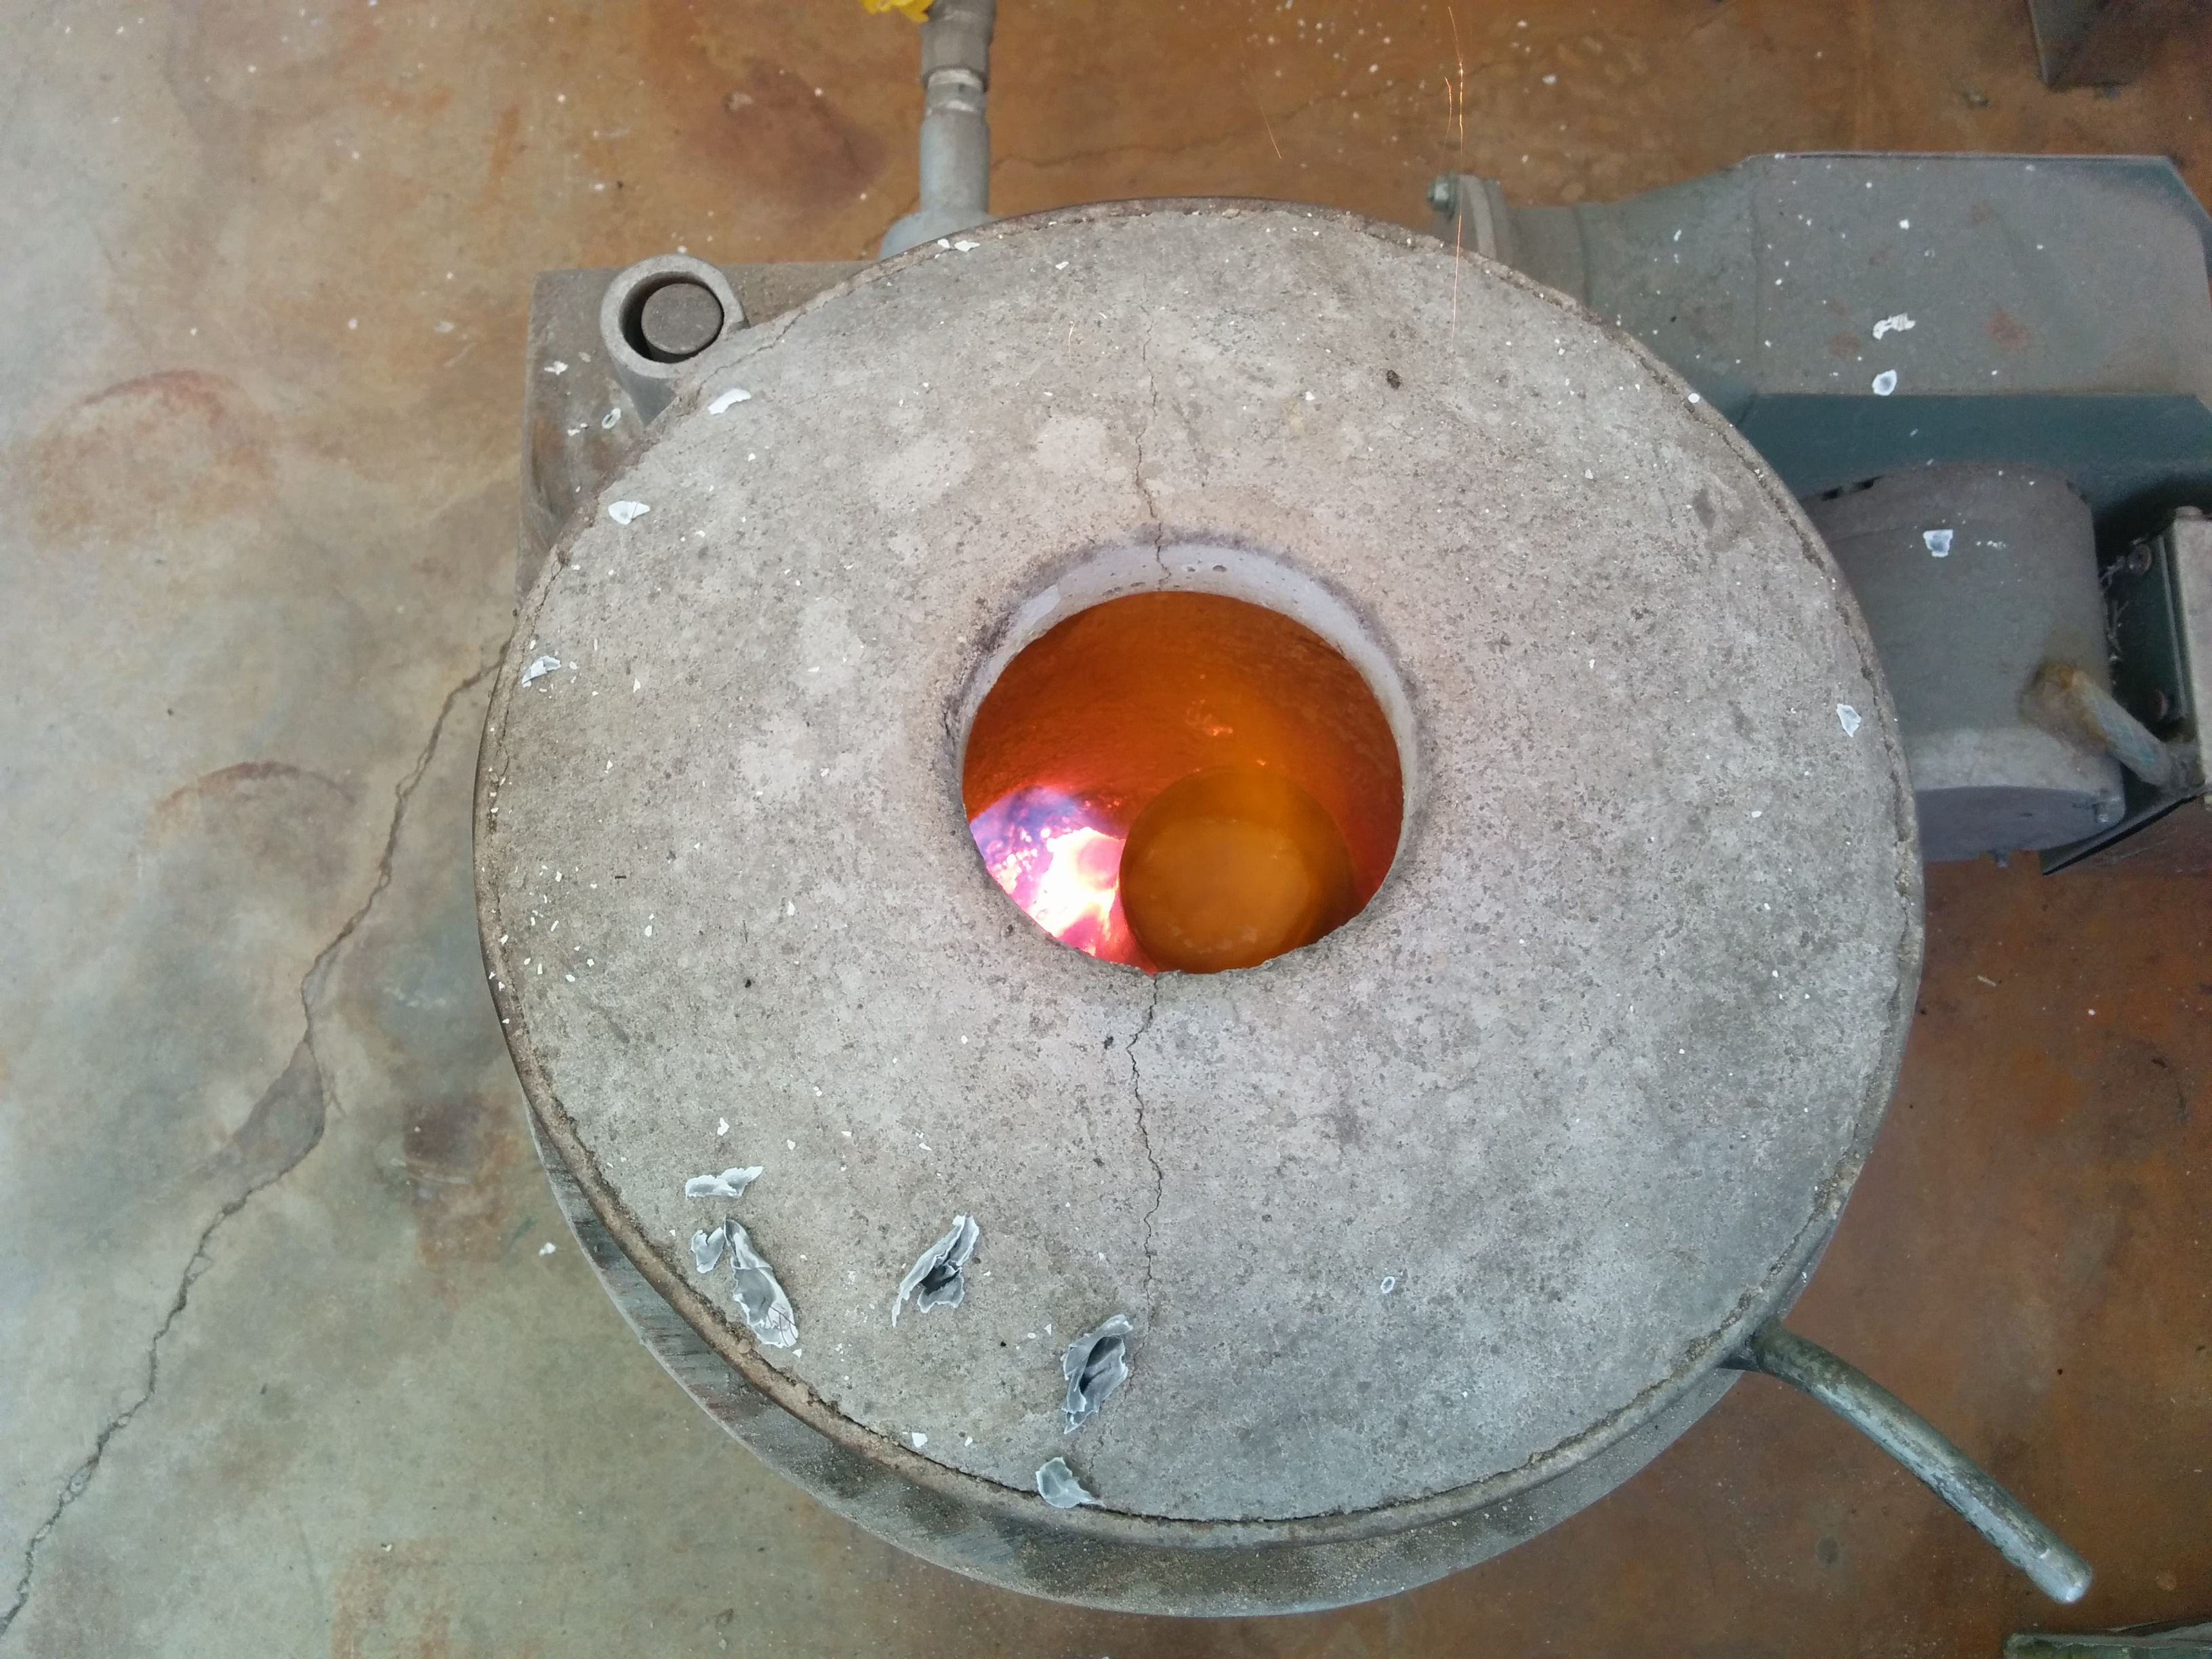
\includegraphics[width=0.7\textwidth]{forno}
		\caption{Mistura de sais sendo aquecida e fundida no forno à gás.}
		\label{fig:forno}
	\end{figure}

	\begin{figure}[H]
		\centering
		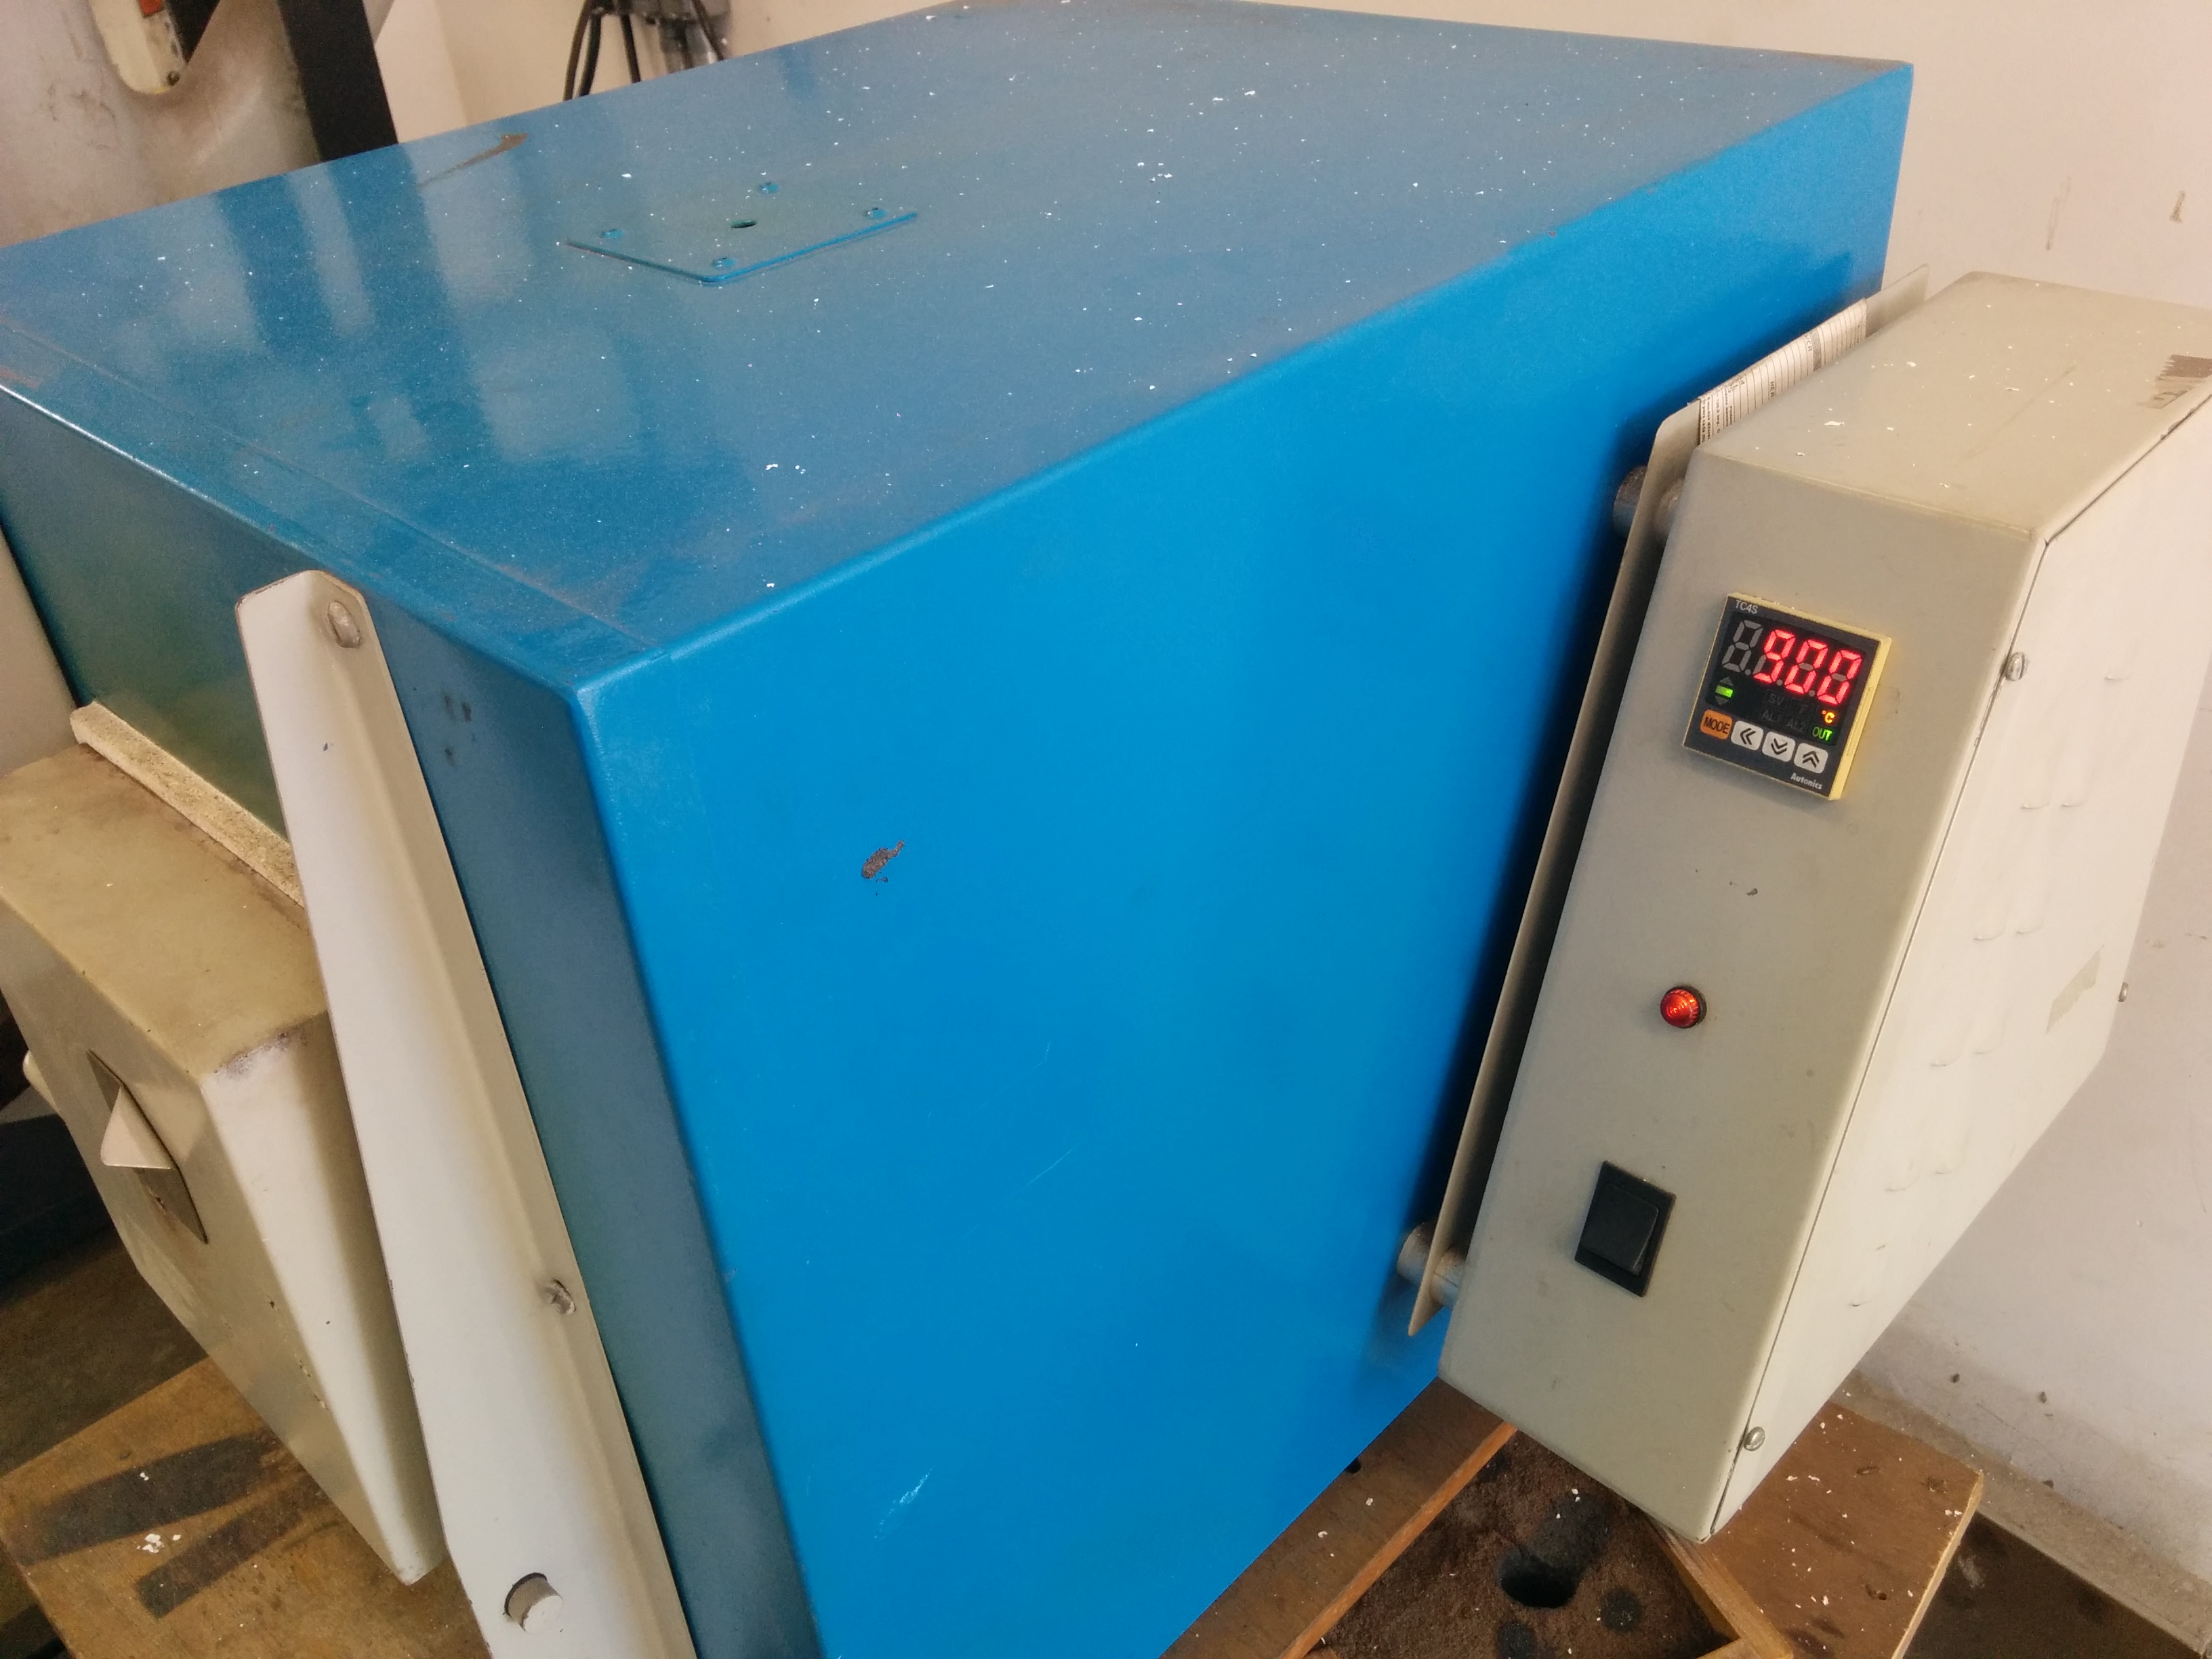
\includegraphics[width=0.7\textwidth]{mufla}
		\caption{Corpos de prova sendo aquecidos acima da temperatura de austenitização, à 900$^{\circ}$C.}
		\label{fig:mufla}
	\end{figure}

	Após o aquecimento dos corpos de prova e dos sais até as temperaturas desejadas, a amostra foi resfriada nos sais por 5 min (Fig. \ref{fig:resfriamento}), conforme a linha 2 da Fig. \ref{fig:austempera}.
	
	\begin{figure}[H]
		\centering
		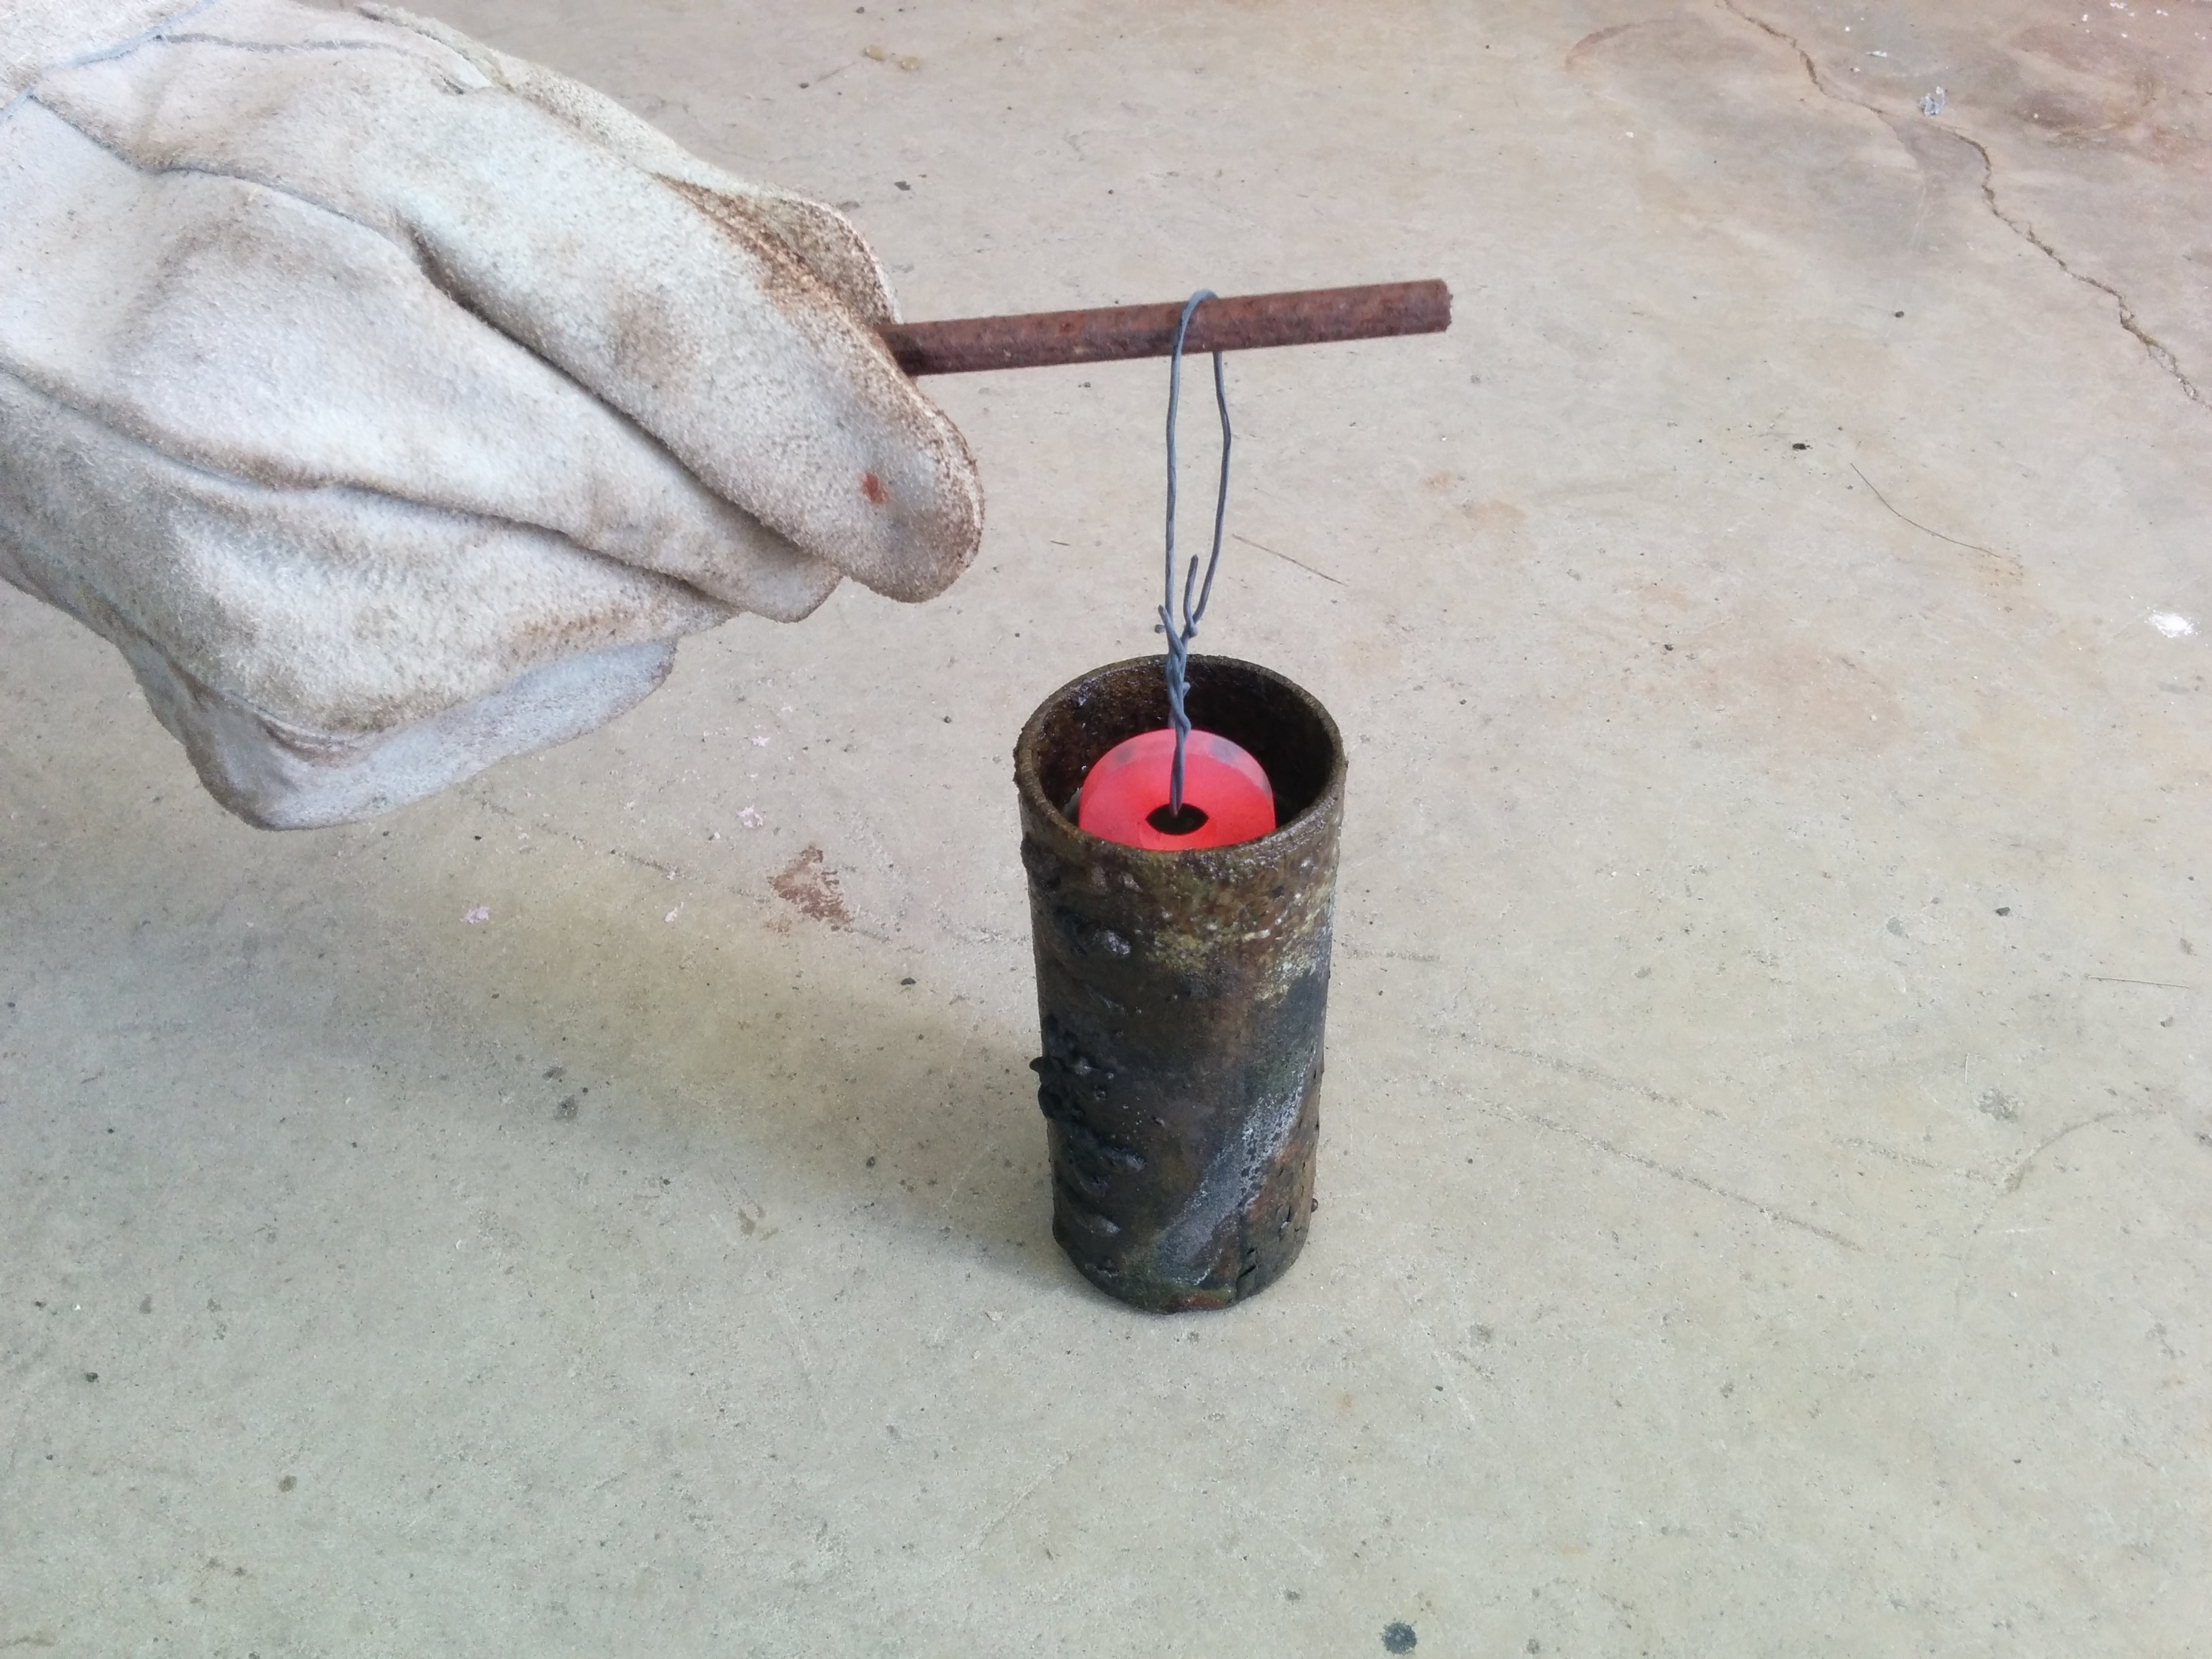
\includegraphics[width=0.7\textwidth]{resfriamento}
		\caption{Amostra de roda sendo resfriada no banho de sais à 380$^{\circ}$C.}
		\label{fig:resfriamento}
	\end{figure}

	A Tabela \ref{tab:parametros_austempera} mostra um resumo dos parâmetros utilizados para a realização da austêmpera.
	
	\begin{table}[H]
		\centering
		\caption{Parâmetros utilizados na austêmpera.}
		\begin{tabular}{|cc|}
			\hline
			\multicolumn{2}{|c|}{Austêmpera} \bigstrut\\
			\hline
			Temperatura de aquecimento da peça & 900$^\circ$C \bigstrut[t]\\
			Tempo de aquecimento da peça & 15 min \\
			Temperatura do banho de sais & 380$^\circ$C \\
			Tempo de resfriamento no banho de sais & 5 min \\
			Tipo de banho & Nitrato de potássio e nitrito de sódio \bigstrut[b]\\
			\hline
		\end{tabular}%
		\label{tab:parametros_austempera}%
	\end{table}%
	

	O banho térmico das amostras no sal foi realizado individualmente para cada amostra para se evitar um superaquecimento do sal e consequentemente uma transformação isotérmica fora da temperatura desejada. Durante toda a operação, foi feito o monitoramento de temperatura do sal através de um pirômetro, conforme a Fig. \ref{fig:pirometro}, a fim de se manter a temperatura o mais próximo possível da temperatura ideal de 380$^{\circ}$C. Quando muito elevada a temperatura do sal, esperou-se o sal trocar temperatura com o próprio ambiente, e, quando muito baixa a temperatura do sal, levou-se novamente ao forno para um reaquecimento.
	
	\begin{figure}[H]
		\centering
		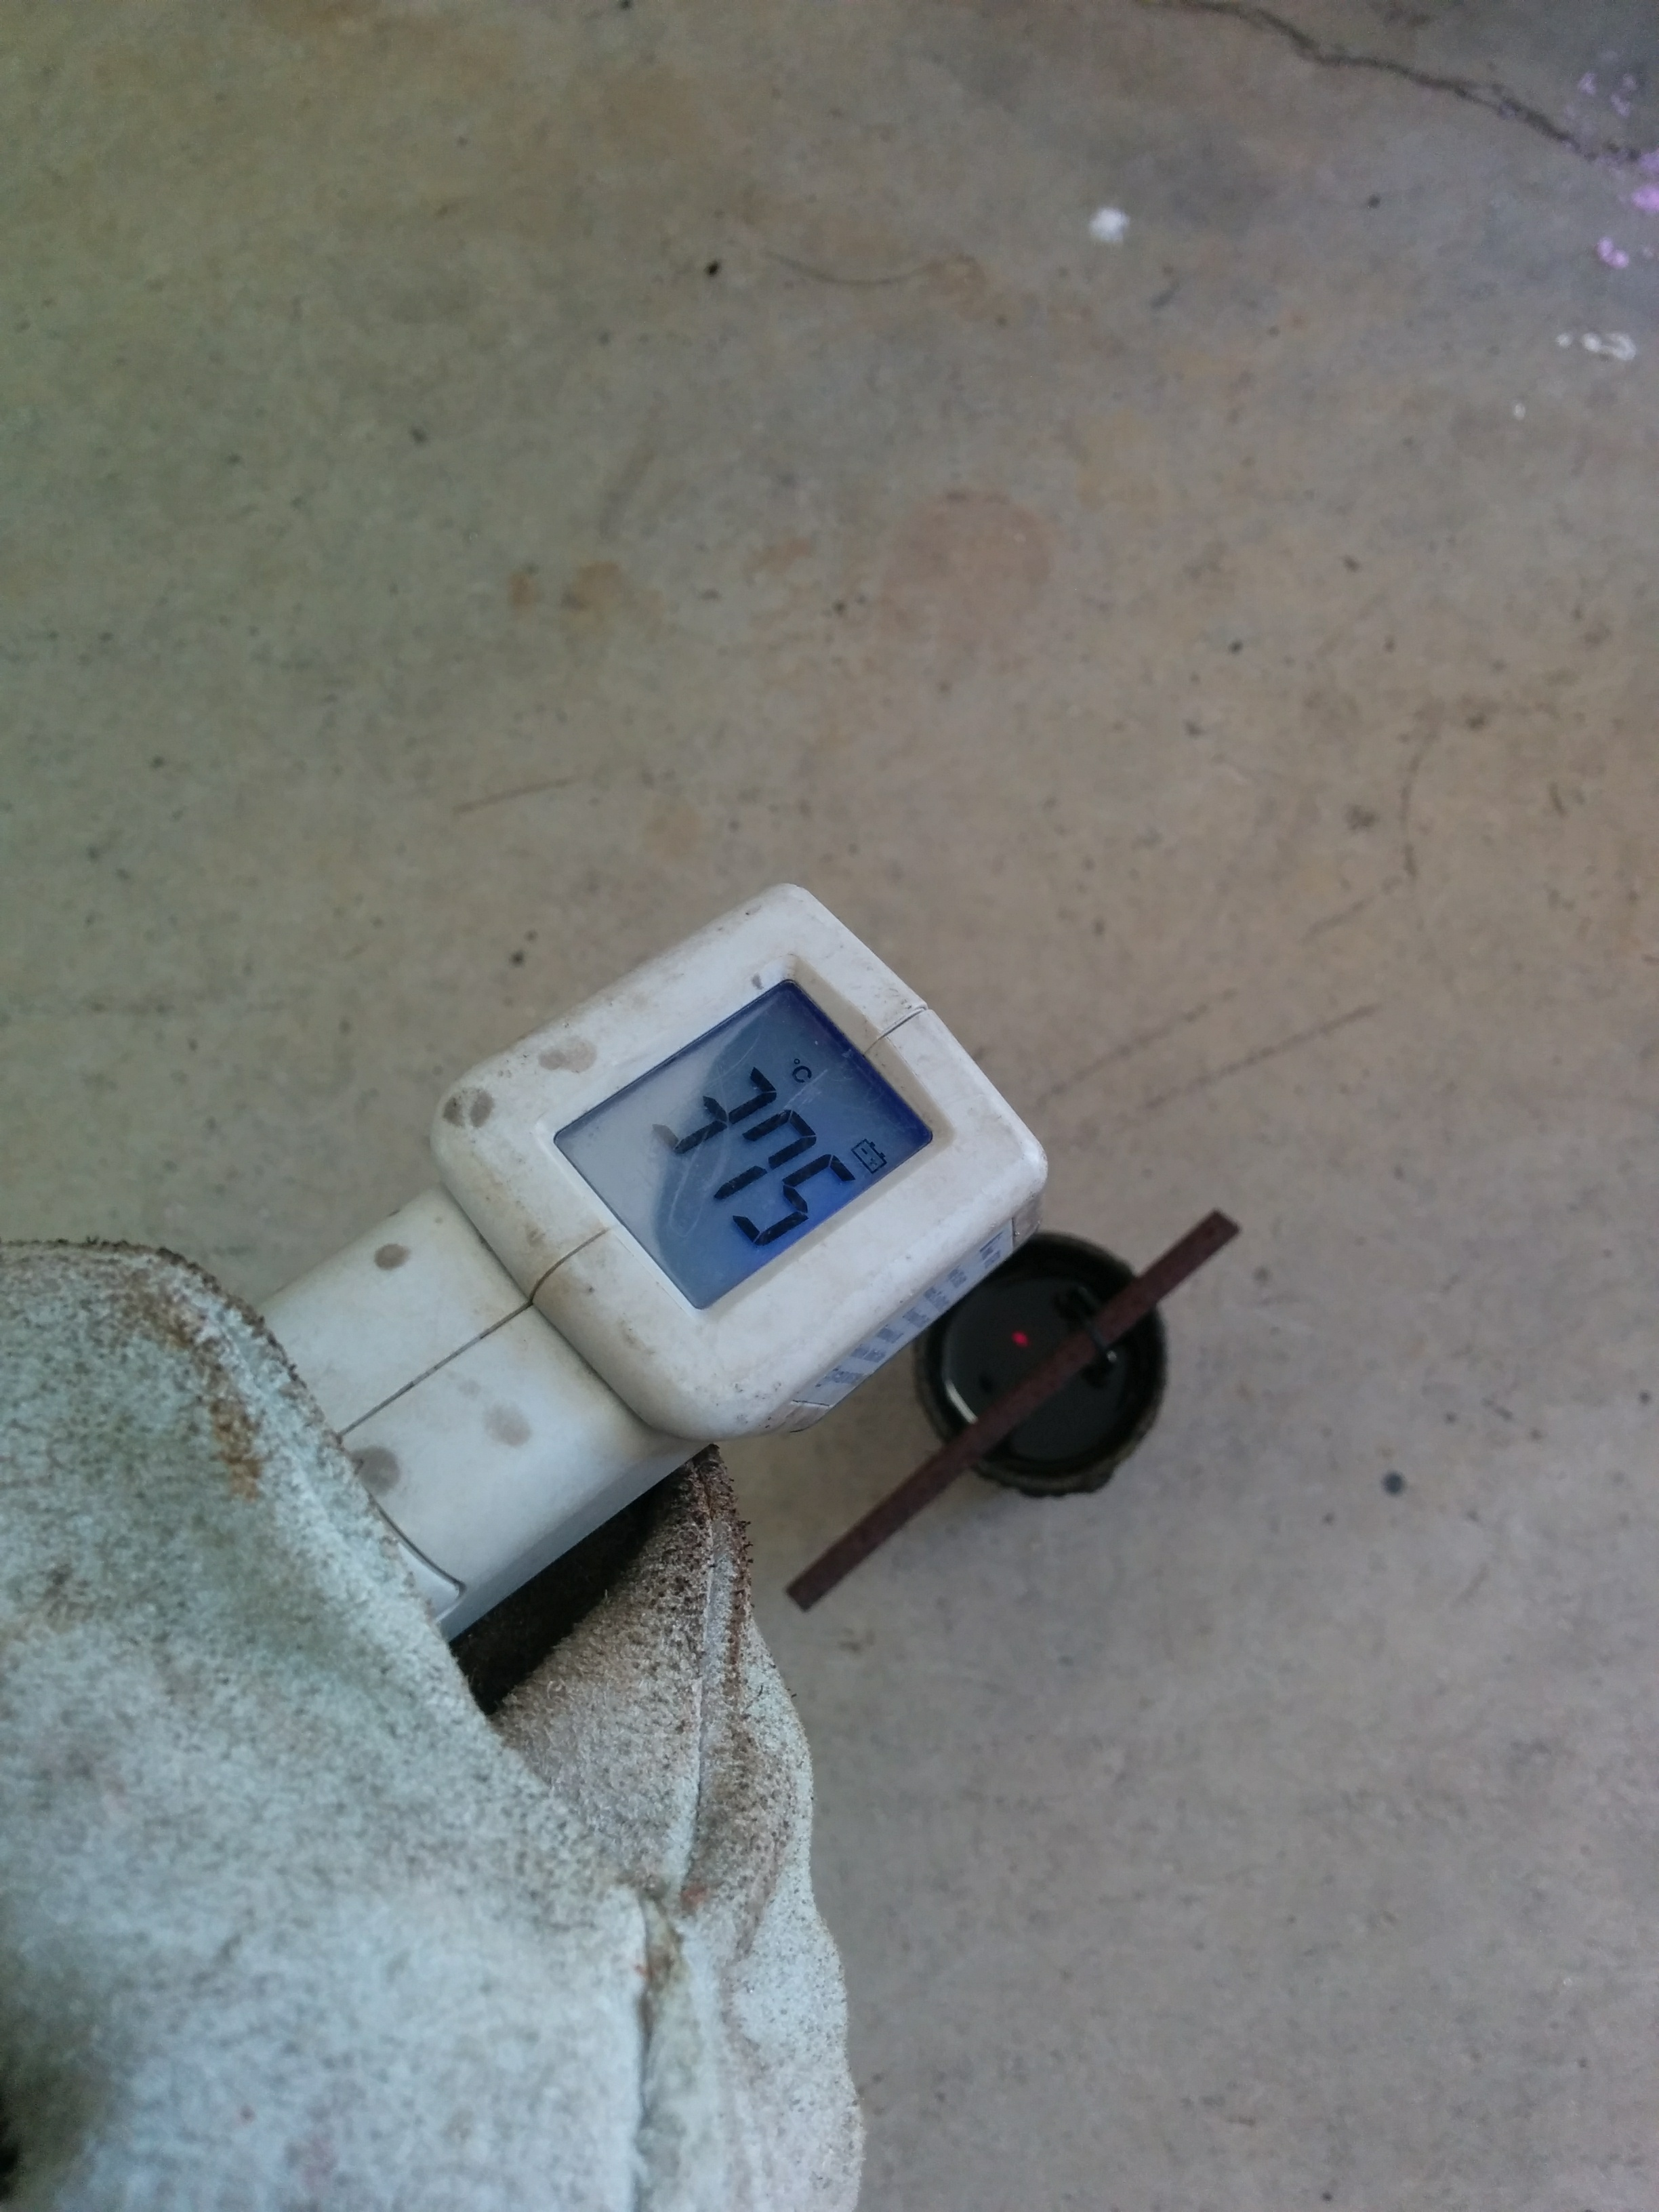
\includegraphics[width=0.6\textwidth]{pirometro}
		\caption{Monitoramento de temperatura feito através de um pirômetro.}
		\label{fig:pirometro}
	\end{figure}

	Após o tratamento, as rodas bainíticas apresentaram uma camada escura de óxido que se formou no tratamento térmico, conforme visualizado na Fig. \ref{fig:amostra_bainita}.
	
	\begin{figure}[H]
		\centering
		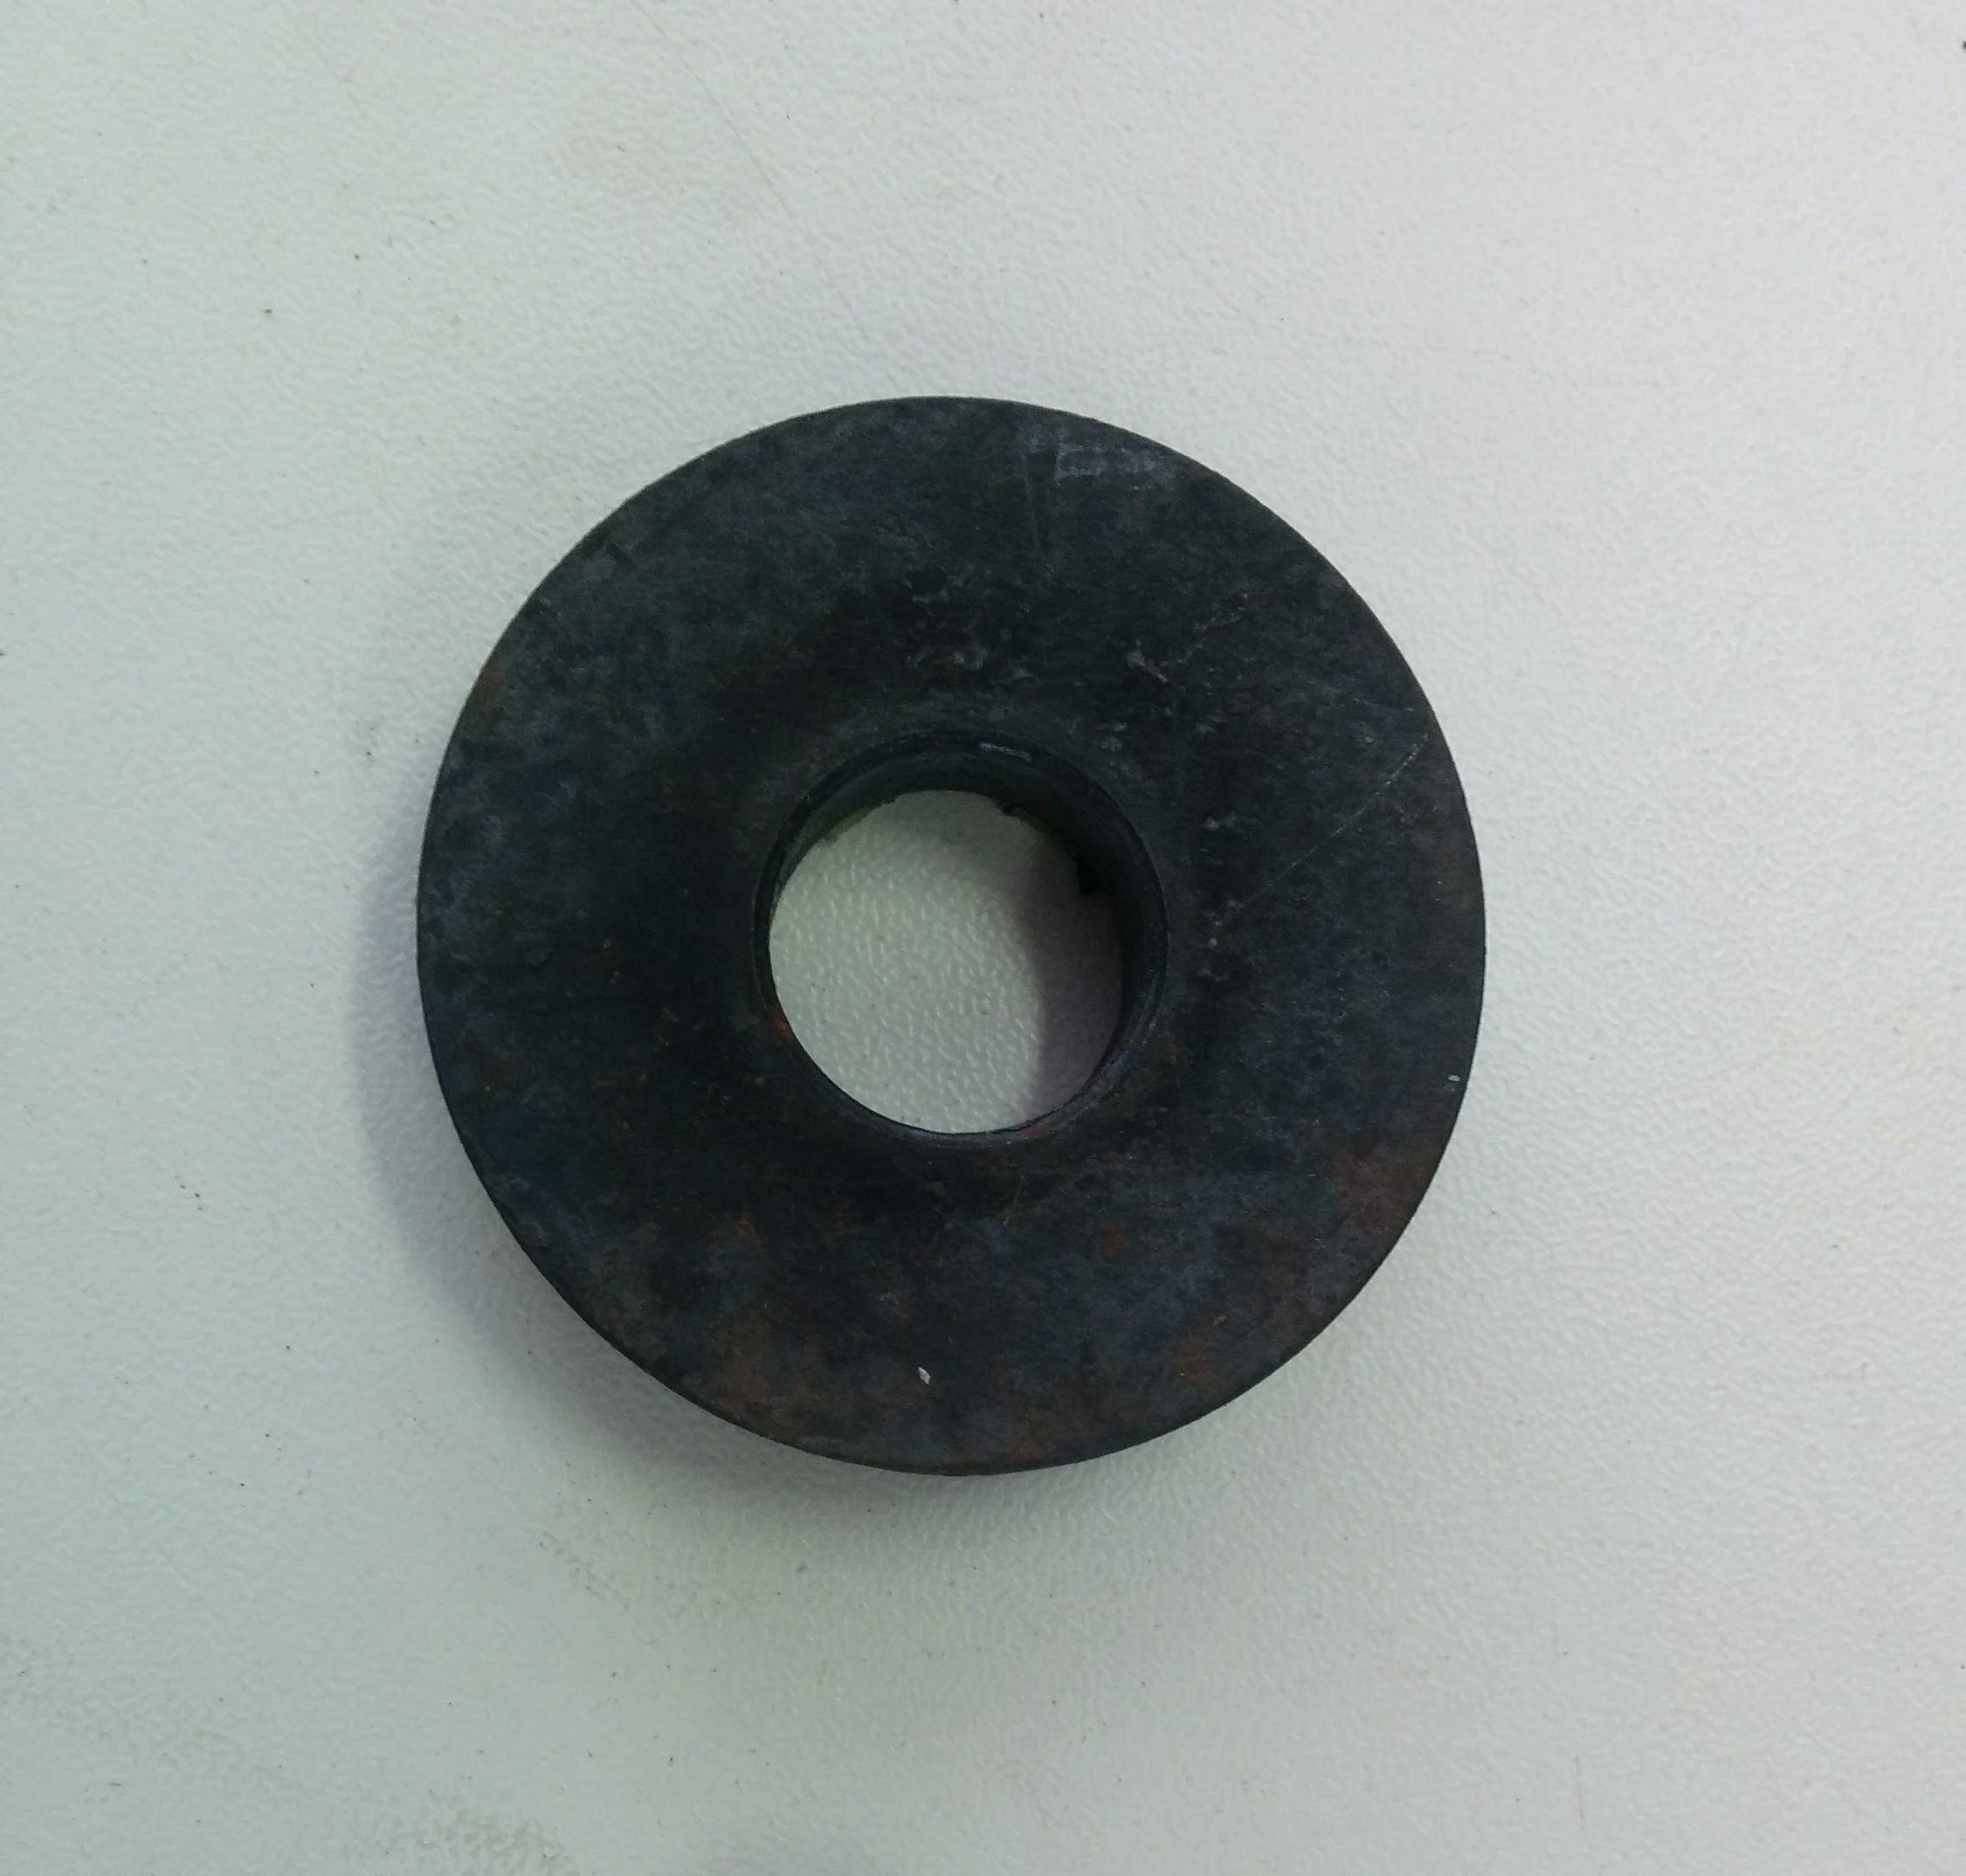
\includegraphics[width=0.7\textwidth]{amostra_bainita}
		\caption{Amostra de bainita pós-austêmpera com camada escura de revestimento.}
		\label{fig:amostra_bainita}
	\end{figure}

	As rodas foram, então, usinadas novamente para a retirada da camada escura de óxido, que poderia influenciar negativamente nos resultados dos ensaios de desgaste, e para a obtenção do formato padrão, com diâmetro externo de 39 mm e diâmetro interno de 15 mm.
	
	O rolamento ainda não foi acoplado ao furo nessa fase, pois o tratamento de revenimento ainda fora necessário para se reduzir a dureza da amostra, que foi elevada através do próprio tratamento de austêmpera.

\pagebreak	
\section{Análise de dureza}

	Após o tratamento térmico de austêmpera, foi realizado o teste de dureza por penetração em todas amostras perlíticas e bainíticas. Os ensaios de dureza foram realizados em um durômetro Equilam, modelo EQTSM, que realiza testes em diversas escalas Rockwell.
	
	A escala Rockwell C foi utilizada para a medição direta da dureza, escala essa que é adequada para o teste de dureza de diversas gamas de aços, inclusive os de composição eutetóide. Para o teste Rockwell C, é utilizado um penetrador com ponta cônica de diamante, uma carga maior de 150 kgf e uma pré-carga padrão de 10 kgf.
	
	Os resultados dos testes de dureza pós-austêmpera e suas análises estão dispostos na seção \ref{sec:analise_dureza_pos_austempera}.
	
	

\pagebreak	
\section{Revenido}
\label{sec:revenido}
	No processo de austêmpera, a formação da microestrutura bainítica aumenta consideravelmente a dureza do aço. Tendo em vista o objetivo de comparar duas microestruturas distintas (perlita e bainita), é necessária a fixação de uma dureza comum entre as microestruturas para que seja realizado o ensaio de desgaste, pois, conforme Archard \cite{archard1953contact}, pela Eq. \ref{eq:archard}, a taxa de desgaste varia de forma inversamente proporcional à dureza do material. 
	
	\begin{equation} \label{eq:archard}
	Q = K\frac{W}{H}
	\end{equation}
	
	A Equação \ref{eq:archard} é conhecida como a Equação de Desgaste de Archard e evidencia as principais variáveis que influenciam no desgaste; e também fornece uma maneira de descrever a severidade do desgaste, através de uma constante K de desgaste. Na Equação de Archard, Q representa o volume total de material perdido com o atrito por unidade de distância de deslizamento, que é obtido através da pesagem após o teste no tribômetro. As variáveis H e W representam, respectivamente, a dureza do material mais macio e a carga aplicada para o contato entre eles.
	
	Para fixar, portanto, uma dureza comum das amostras a fim de comparação, realizou-se o tratamento térmico de revenimento nos corpos de prova que foram austemperados, que se consiste em reaquecer o corpo de prova a uma temperatura muito inferior à da fase de austenitização e manter sob tal temperatura por um intervalo de tempo.

	Nessa etapa, objetivou-se reduzir a dureza dos corpos de prova de bainita, que foi consideravelmente elevada devido à austêmpera. A dureza deve ser reduzida até àquela dos corpos perlíticos puros não tratados (aproximadamente 40,5 HRC, segundo a Tab. \ref{tab:dureza_pos_austempera}). Para isso, foi utilizada a mufla do Laboratório de Processo de Fabricação, configurando a temperatura para que se estabilizasse a 500$^\circ$C. Após atingida a temperatura estabelecida, colocou-se todos os corpos de prova de bainita. Os materiais permaneceram no forno por 20 min e, logo em seguida, foram resfriados com água, para evitar a fragilização no revenido \cite{silva2006acos}.

	Logo em seguida ao tratamento térmico de revenimento, foi realizado o ensaio de dureza dos três corpos de bainita revenida; e também no contracorpo (correspondente ao material do trilho). Os dados de dureza dos corpos de perlita também foram refeitos através de novas medições.
	
	Os dados das medições de dureza dos corpos de bainita (pós-revenido) e de perlita; e das leituras de dureza para o contracorpo estão expressos na seção \ref{sec:analise_dureza_pos_revenido}.

\section{Micrografia}	

	A micrografia, neste estudo, foi realizada após o teste de dureza com o objetivo de se investigar os detalhes da microestrutura das amostras bainíticas e assegurar que o material foi tratado termicamente de maneira correta. Para as amostras perlíticas também foi realizada a micrografia, porém com o objetivo de atestar que a microestrutura ali presente de fato é a perlita fina.

	As fotos obtidas pela micrografia foram, então, analisadas e comparadas com imagens obtidas na literatura, de tamanhos e formas microestruturais clássicas, tanto para a perlita como para a bainita.

	Para se observar a microestrutura superficial dos corpos de prova, uma das 3 amostras bainíticas e uma das 3 amostras perlíticas foram cortadas em uma serra circular com fluido refrigerante. O corte foi feito estrategicamente conforme a Fig. \ref{fig:corte_micrografia}  para que se consiga fazer uma obervação da forma e tamanho do grão no centro do corpo de prova.

	\begin{figure}[H]
		\centering
		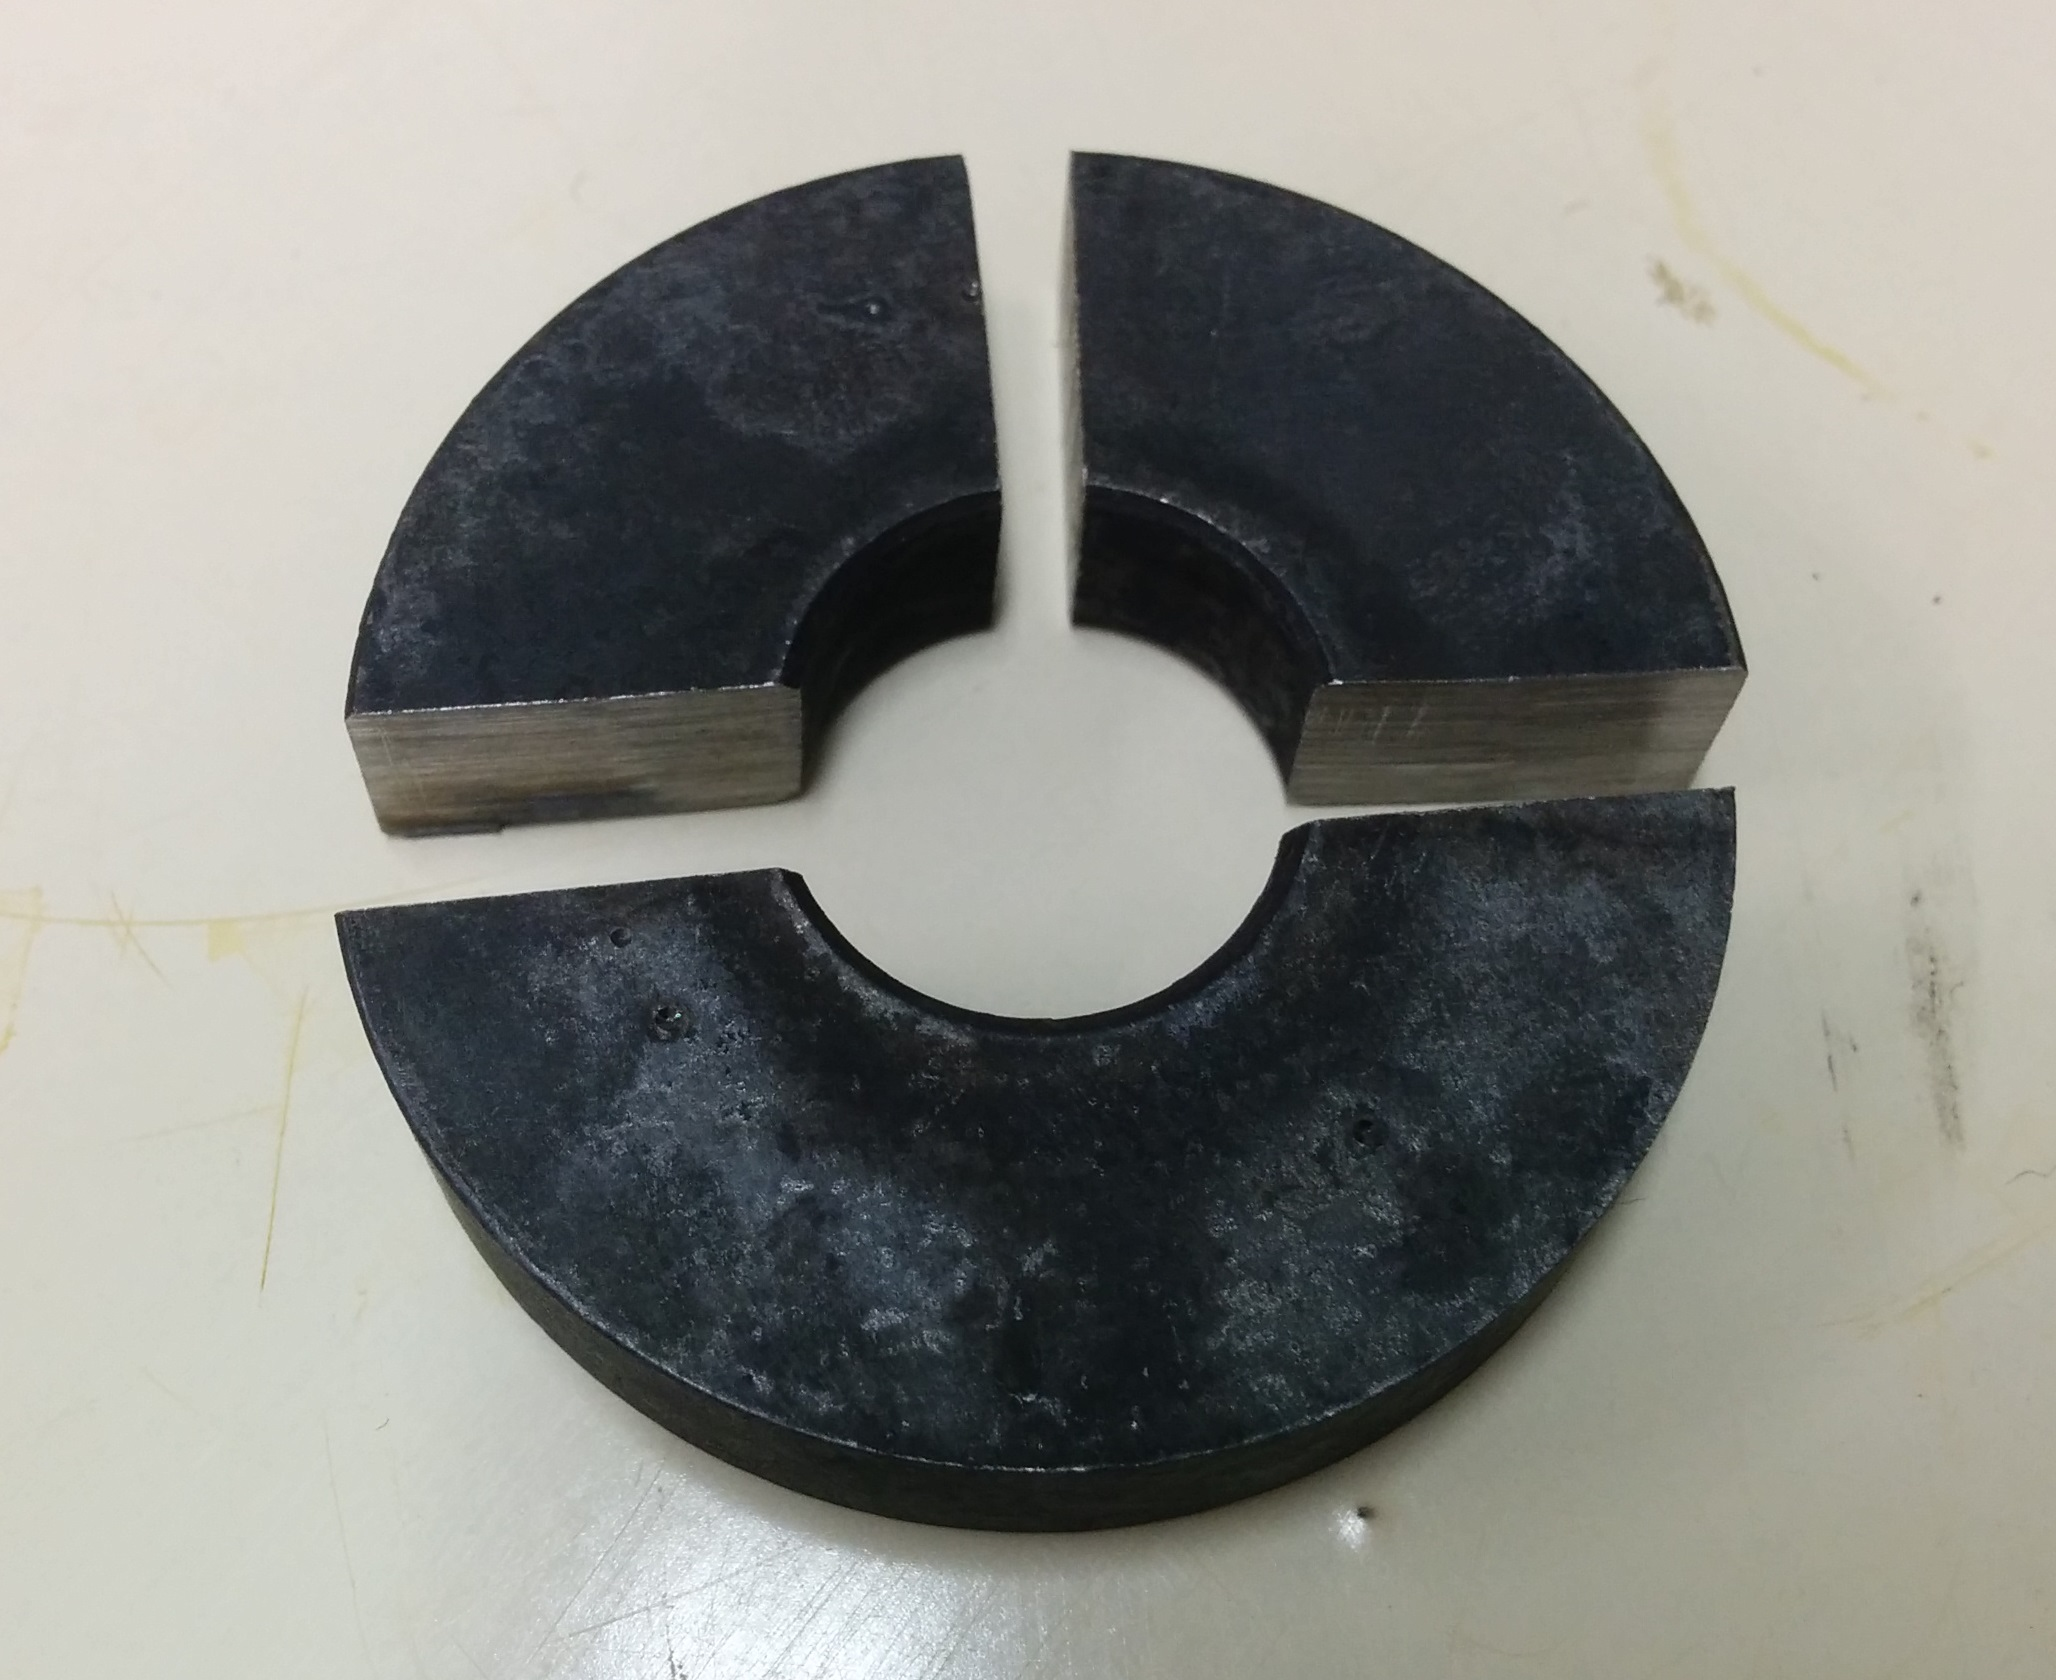
\includegraphics[width=0.4\textwidth]{corte_micrografia}
		\caption{Esquema de corte da amostra para sua análise microestrutural.}
		\label{fig:corte_micrografia}
	\end{figure}
	
	Para a análise de todas as amostras, foi utilizado como ferramenta para investigação a microscopia eletrônica de varredura (MEV). Os corpos de provas cortados foram levados ao Laboratório de Fenômenos de Superfície da Universidade de São Paulo (LFS-USP), onde as imagens microestruturais foram feitas.


	\subsection{Imagens microestruturais clássicas}
	\label{sec:imagens_bibliografia}
	
	As imagens das micrografias feitas para as amostras bainíticas e perlíticas foram comparadas com imagens de bainita e perlita clássicas, encontradas na literatura. Tal comparação tem o objetivo de checar se a aparência das amostras de teste de cada uma dessas microestruturas convergem com as características presentes na literatura, com tamanhos e formas microestruturais clássicos, tanto para a perlita como para a bainita.
	
	A Figura \ref{fig:bainita_bib2} demonstra uma imagem obtida na bibliografia do constituinte acicular, bainita.
	
	\begin{figure}[H]
		\centering
		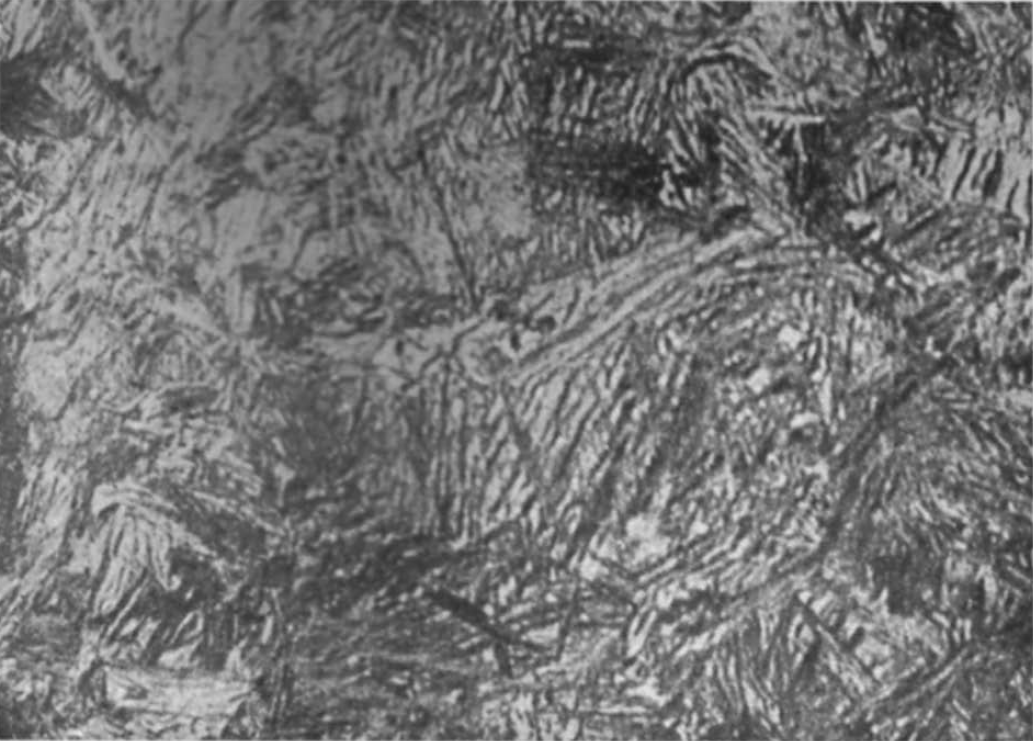
\includegraphics[width=0.73\textwidth]{bainita_bib2}
		\caption{Bainita produzida pela austêmpera de aço em banho de sal a 250$^\circ$C. Ataque: nítrico. Ampliação 750 vezes. \cite{colpaert1994metalografia}}
		\label{fig:bainita_bib2}
	\end{figure}

	Colpaert \cite{colpaert1994metalografia} expõe também imagens de aços revenidos, como o da Fig. \ref{fig:revenido_bib}. Para revenidos em torno de 450$^\circ$C, a mobilidade do carbono cresce e a microestrutura passa a apresentar uma textura característica, denominada sorbíticas \cite{colpaert1994metalografia}, constituída de pequenas partículas de cementita, geralmente tendendo para a forma esferoidal sobre um fundo de ferro $\alpha$ (ferrita) \cite{colpaert1994metalografia}.
	\begin{figure}[H]
		\centering
		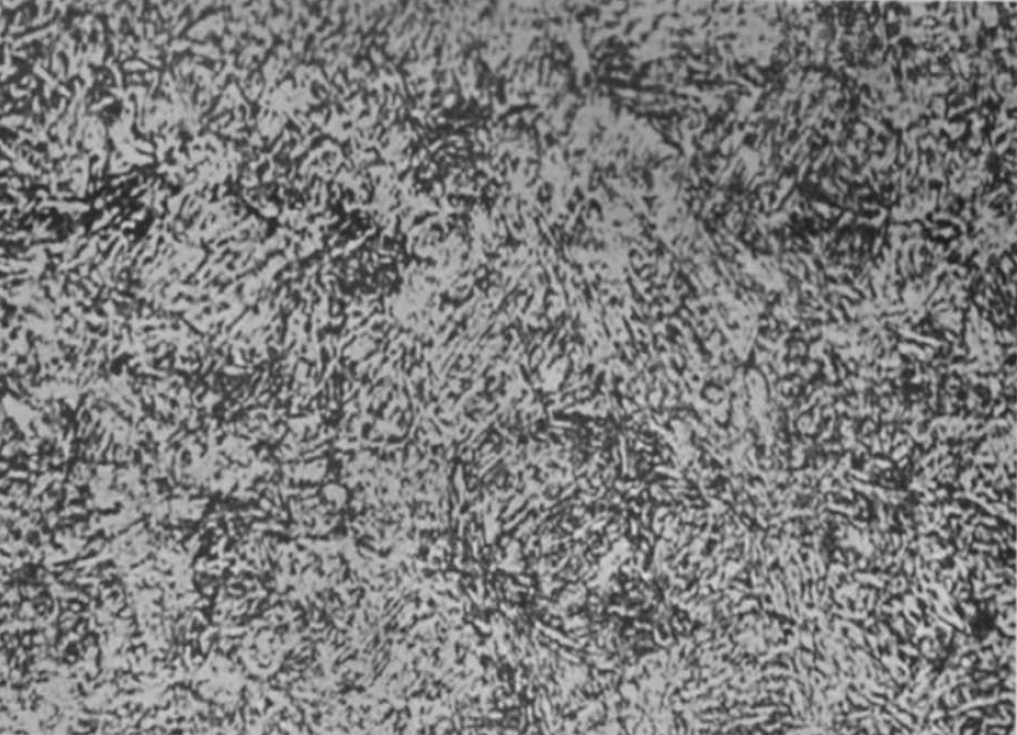
\includegraphics[width=0.73\textwidth]{revenido_bib}
		\caption{Aço com 0,5\% de carbono, temperado em água fria e revenido a 400$^\circ$C. Textura sorbítica com início de formação de pequenos glóbulos de cementita. Ataque: nítrico. Ampliação: 750 vezes. \cite{colpaert1994metalografia}}
		\label{fig:revenido_bib}
	\end{figure}
	
	Já para a microestrutura perlítica, tem-se a Fig. \ref{fig:perlita_bib}, retirada de Colpaert \cite{colpaert1994metalografia}. É uma micrografia referente à perlita fina em um aço eutetóide. A perlita é um constituinte micrográfico do aço, formado por finas lamelas justapostas de ferrita e cementita; e é obtida através de um resfriamento lento a partir da temperatura de austenitização. A espessura das lamelas são, em geral, da ordem de alguns décimos de micrômetros e habitualmente só são visíveis com ampliação de mais de 200 vezes \cite{colpaert1994metalografia}. As lamelas são mais ou menos paralelas e podem ser planas, curvas ou ondeadas \cite{colpaert1994metalografia}.
	
	\begin{figure}[H]
		\centering
		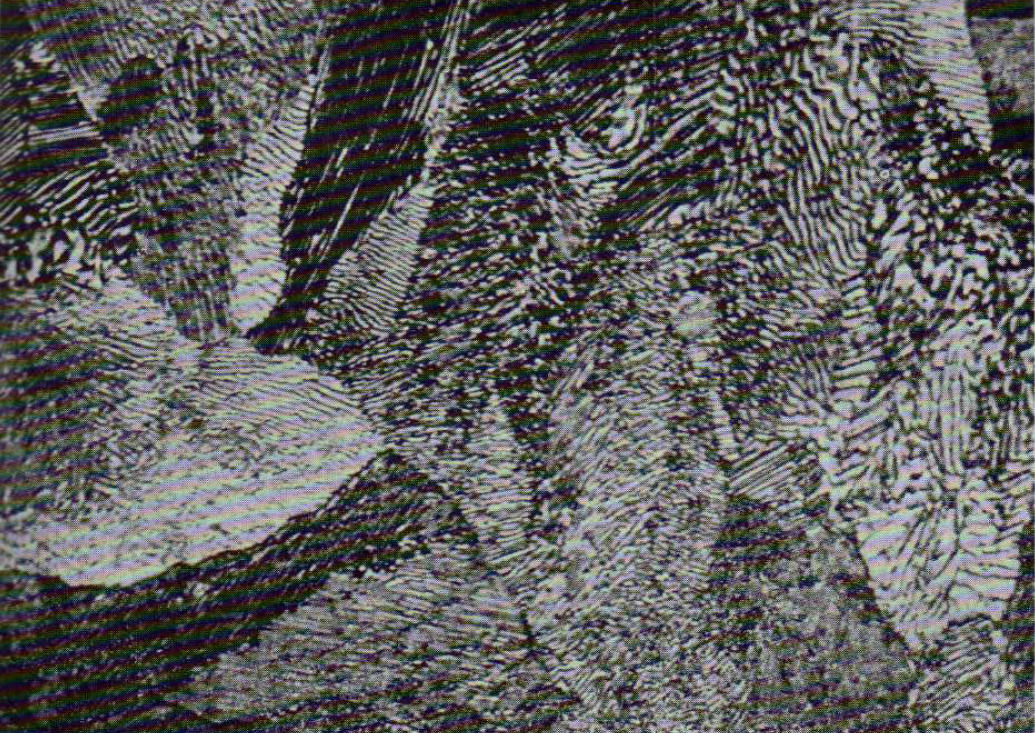
\includegraphics[width=1\textwidth]{perlita_bib}
		\caption{Aço eutetóide. Grãos de perlita, demonstrando a estrutura lamelar. Ataque: nítrico. \cite{colpaert1994metalografia}}
		\label{fig:perlita_bib}
	\end{figure}

	As análises de comparação das micrografias das amostras de teste com as imagens clássicas presentes da literatura são feitas nas seções \ref{sec:micrografia_bainita} e \ref{sec:micrografia_perlita}.
	
	
	

\pagebreak
\section{Ensaio de desgaste}
	O ensaio foi realizado utilizando o tribômetro fabricado na UFJF, possibilitando a simulação do desgaste de uma roda de trem no conjunto rolo contra disco. Nesse tribômetro, a aplicação da carga e fixação dos corpos de prova é realizada por meio de um braço fixado em uma travessa lateral com rosca sem fim. Essa travessa, além de apoiar o braço, também permite o seu deslocamento no sentido transversal ao contracorpo.
	
	O desgaste foi avaliado por perda de massa em função da distância percorrida ou rolada e do tempo de rolamento, sendo os corpos de prova pesados em uma balança com precisão de 0,0001 g. As avaliações por perda de massa foram medidas a cada 1 hora de ensaio. Foram realizadas 3 medições por carga nos dois corpos de prova perlíticos e nos dois corpos de prova bainíticos. A carga foi fixa, 25,4 N, e corresponde à carga obtida com a massa padrão de 5 kg disponível no Laboratório de Metalografia. Os valor da carga corresponde à força aplicada sobre a roda, considerando o sistema de apoio de carga do braço do tribômetro, conforme a Fig. \ref{fig:apoio_tribometro}.
	
	\begin{figure}[H]
		\centering
		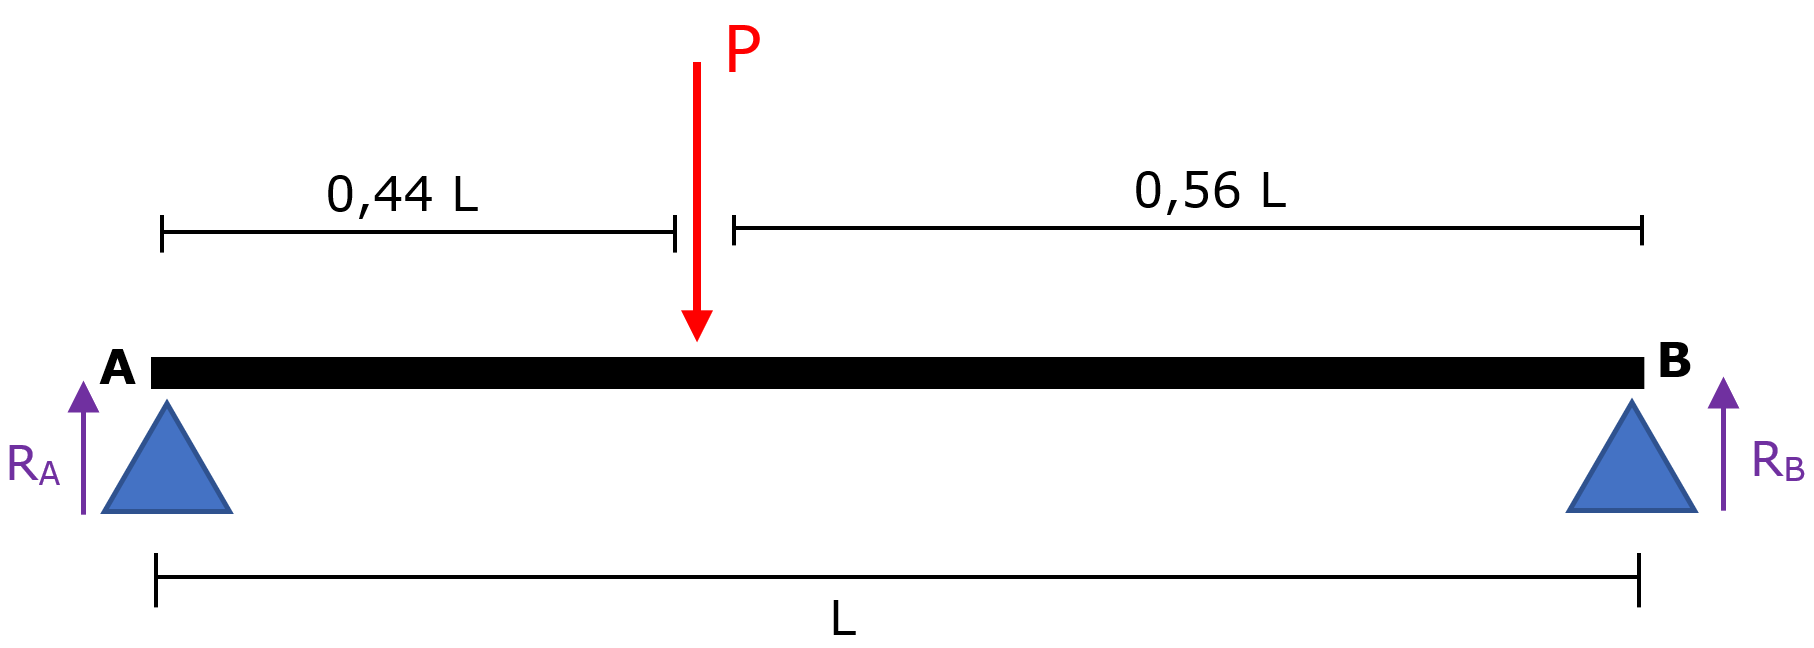
\includegraphics[width=1\textwidth]{apoio_tribometro}
		\caption{Esquema representativo do sistema de apoio do braço do tribômetro. O local de aplicação da força P corresponde ao ponto do pino de apoio de carga, onde a massa é apoiada. O ponto A é o ponto onde o corpo de prova é fixado. A força de reação $R_A$ corresponde à força de contato entre o corpo e o contracorpo.}
		\label{fig:apoio_tribometro}
	\end{figure}

	Os dados de medição da perda de massa para cada teste de 1 hora foram anotados nas Tabs. \ref{tab:perlita1}, \ref{tab:perlita2}, \ref{tab:bainita1} e \ref{tab:bainita2}. A coluna ``Massa da amostra'' representa a leitura da massa aferida na balança de precisão após cada teste e o primeiro valor de massa de cada tabela é a massa inicial da amostra. A coluna ``Perda de massa'' representa a diferença de massa entre a nova leitura e a leitura anterior. 
	
	A taxa de desgaste foi calculada na unidade $[{g.h}/m]$ e foi obtida por meio da Eq. \ref{eq:taxa_de_desgaste}, onde ``Q'' é a taxa de desgaste, ``m'' é a perda de massa, obtida diretamente a partir das Tabs. \ref{tab:perlita1}, \ref{tab:perlita2}, \ref{tab:bainita1} e \ref{tab:bainita2} e ``t'' é o tempo de duração de cada teste, ou tempo de rolamento. O fator no denominador da Eq. \ref{eq:taxa_de_desgaste} é a distância rolada e foi obtida em função da rotação ``n'' do disco do tribômetro e a posição radial ``r'' da roda em relação ao centro do disco.
	

	\begin{equation} \label{eq:taxa_de_desgaste}
	Q = \frac{m.t}{n.\frac{2.\pi.r}{60}}
	\end{equation}

	
	As constantes da Eq. \ref{eq:taxa_de_desgaste} estão representadas na Tab. \ref{tab:constantes}.
	% Table generated by Excel2LaTeX from sheet 'Sheet1'
	\begin{table}[H]
		\centering
		\caption{Constantes utilizadas no cálculo da taxa de desgaste.}
		\begin{tabular}{|cc|}
			\hline
			\multicolumn{2}{|c|}{\textbf{Constantes}} \bigstrut\\
			\hline
			Rotação (n) [rpm] & 433 \bigstrut[t]\\
			Distância do centro (r) [m] & 0,042 \\
			Tempo (t) [h] & 1 \bigstrut[b]\\
			\hline
		\end{tabular}%
		\label{tab:constantes}%
	\end{table}%
	
	
	Para o procedimento de pesagem, após cada teste de 1 hora, as amostras foram inicialmente lavadas em lavadora ultrassônica por 5 min com o objetivo de remover quaisquer impurezas ou detritos de desgaste que ainda não haviam se soltado da peça. As lavadoras ultrassônicas são equipamentos que funcionam através do fenômeno da cavitação, são destinadas ao auxílio na limpeza de partes, retirando todas impurezas nas reentrâncias minúsculas e mais profundas. A Figura \ref{fig:ultrassom} mostra a lavadora ultrassônica utilizada no ensaio.
	
	\begin{figure}[H]
		\centering
		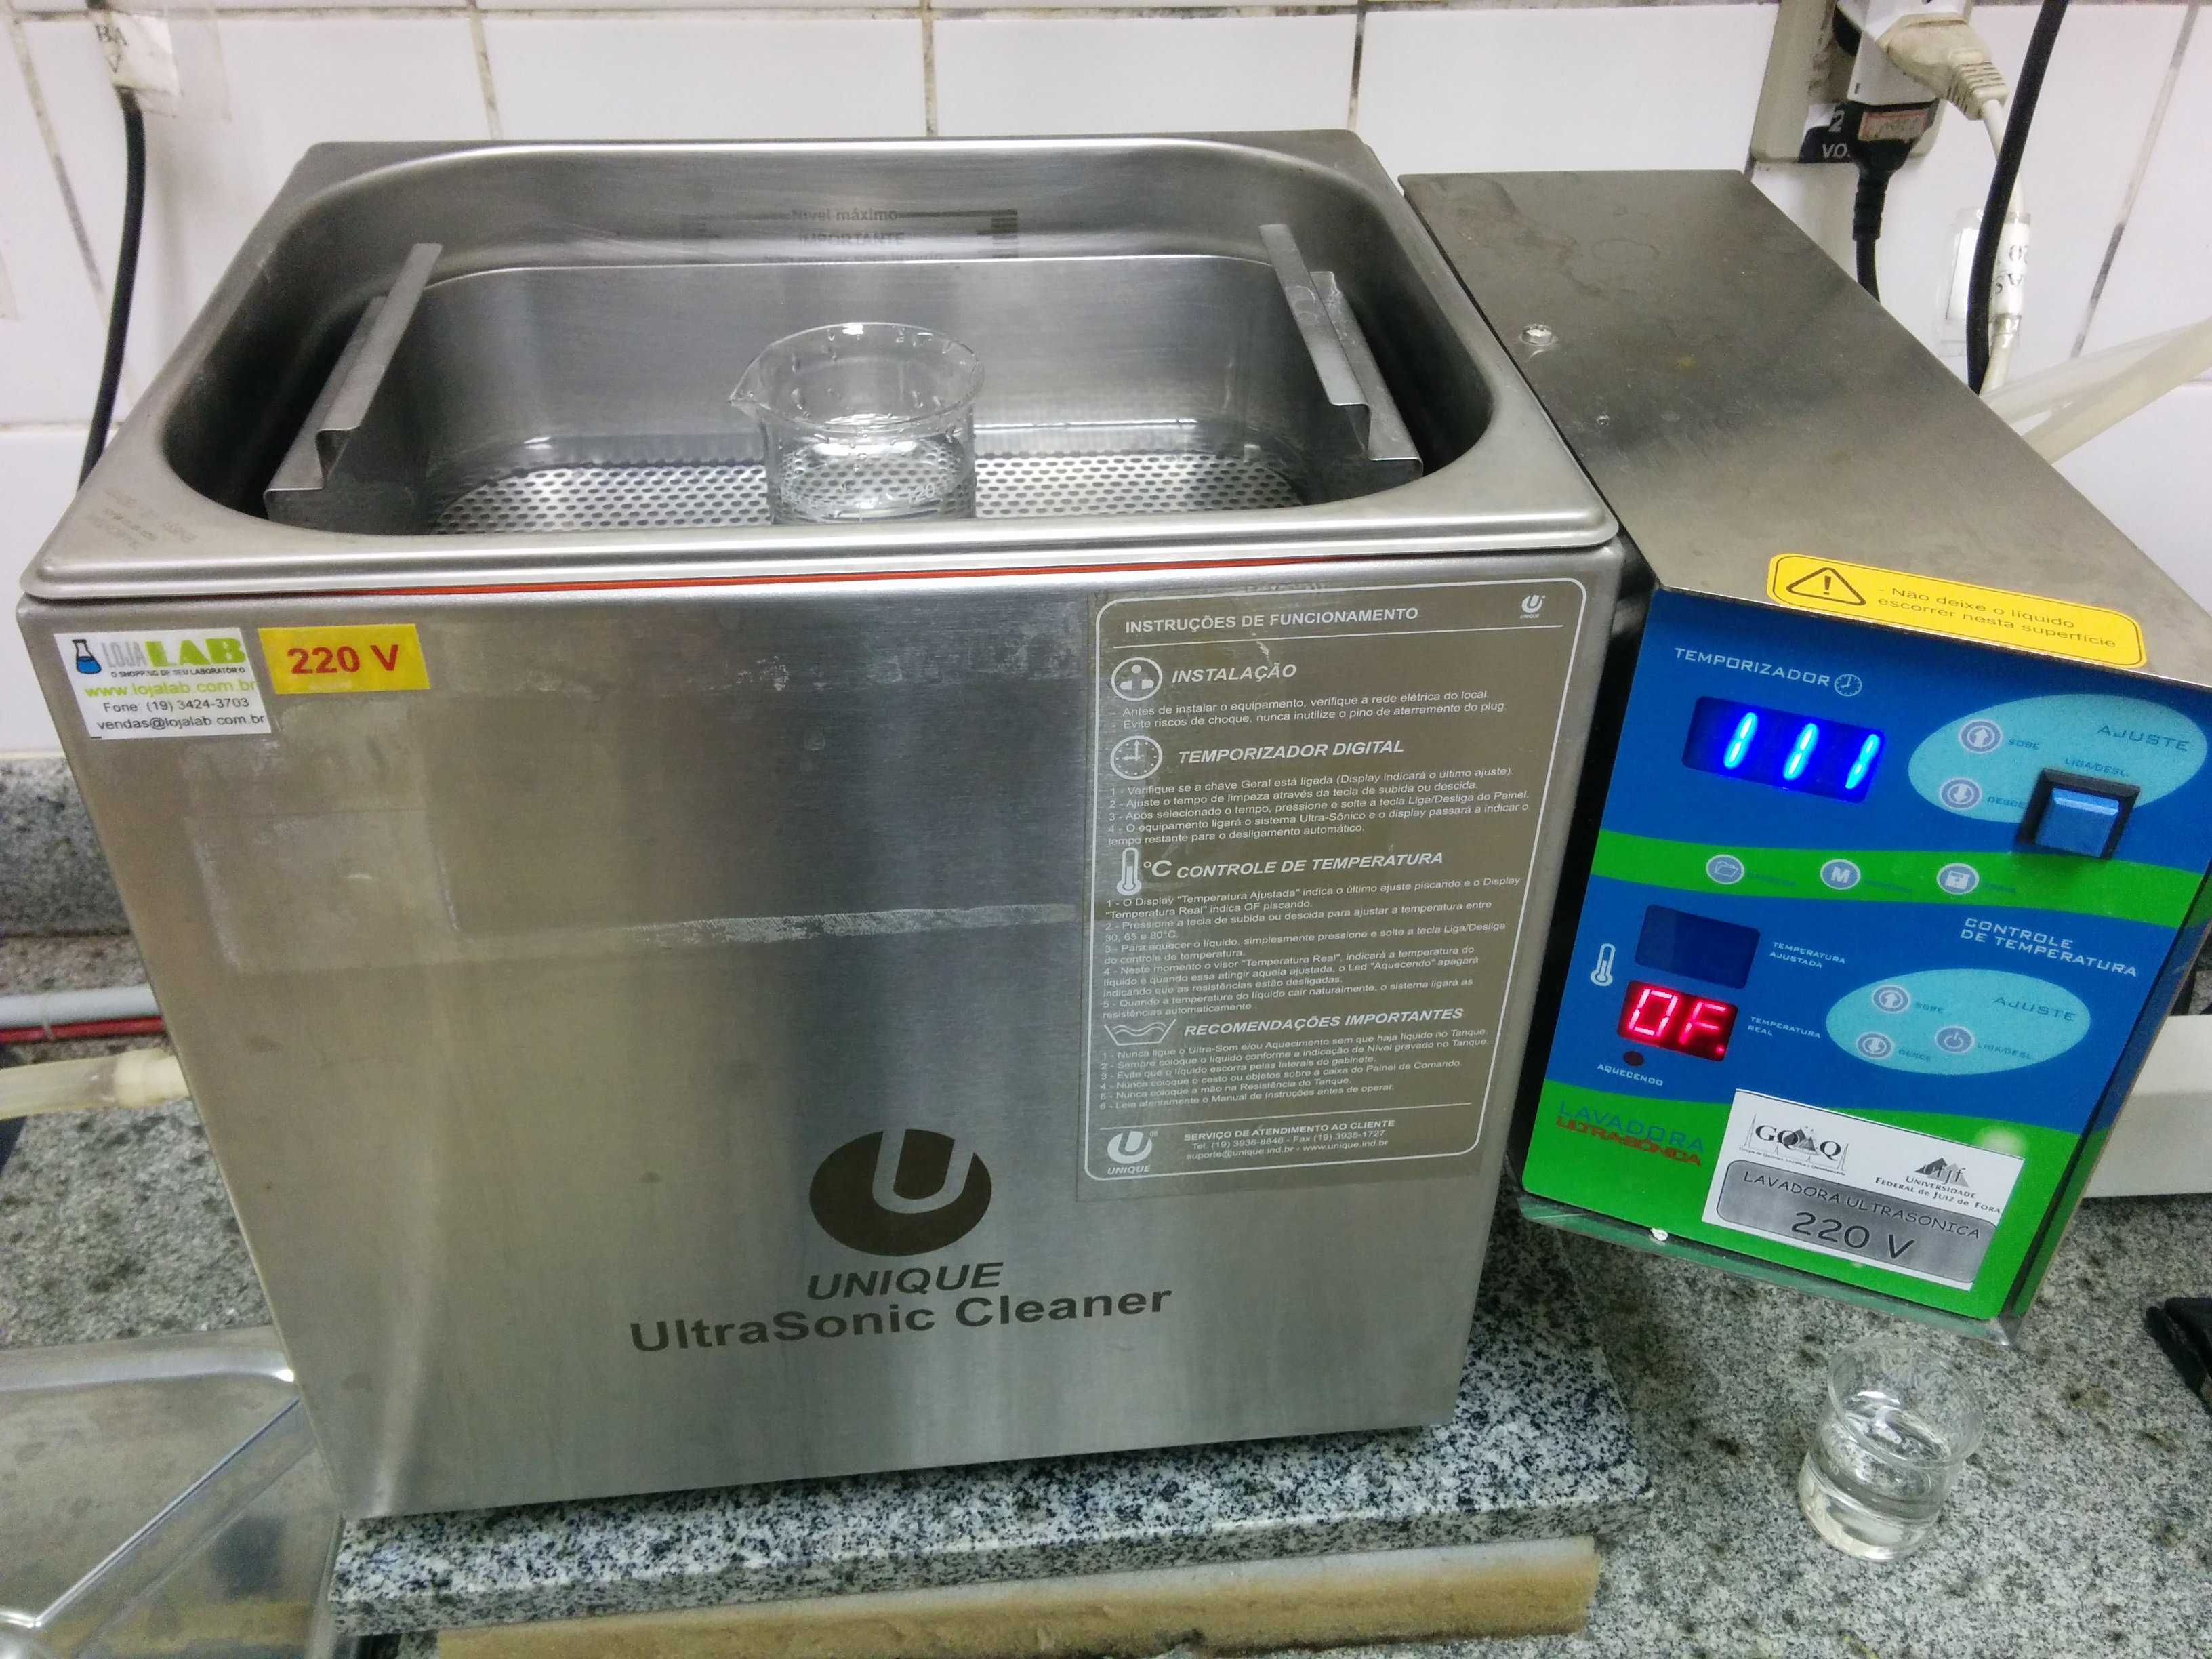
\includegraphics[width=0.8\textwidth]{ultrassom}
		\caption{Lavadora ultrassônica utilizada para limpeza dos corpos de prova antes da pesagem.}
		\label{fig:ultrassom}
	\end{figure}
	
	As pesagens foram realizadas no instante logo após à limpeza das amostras no ultrassom para que não adquiram impurezas do ar atmosférico. A pesagem foi feita em uma balança analítica, com precisão de 0,0001 g, no laboratório da pós-graduação em química da Universidade Federal de Juiz de Fora (UFJF). Esse tipo de equipamento possui um dispositivo tipo capela com três portas para proteger de correntes de ar que podem alterar o valor absoluto da pesagem. A Figura \ref{fig:balanca} mostra a balança analítica utilizada nos procedimentos de pesagem.
	
	\begin{figure}[H]
		\centering
		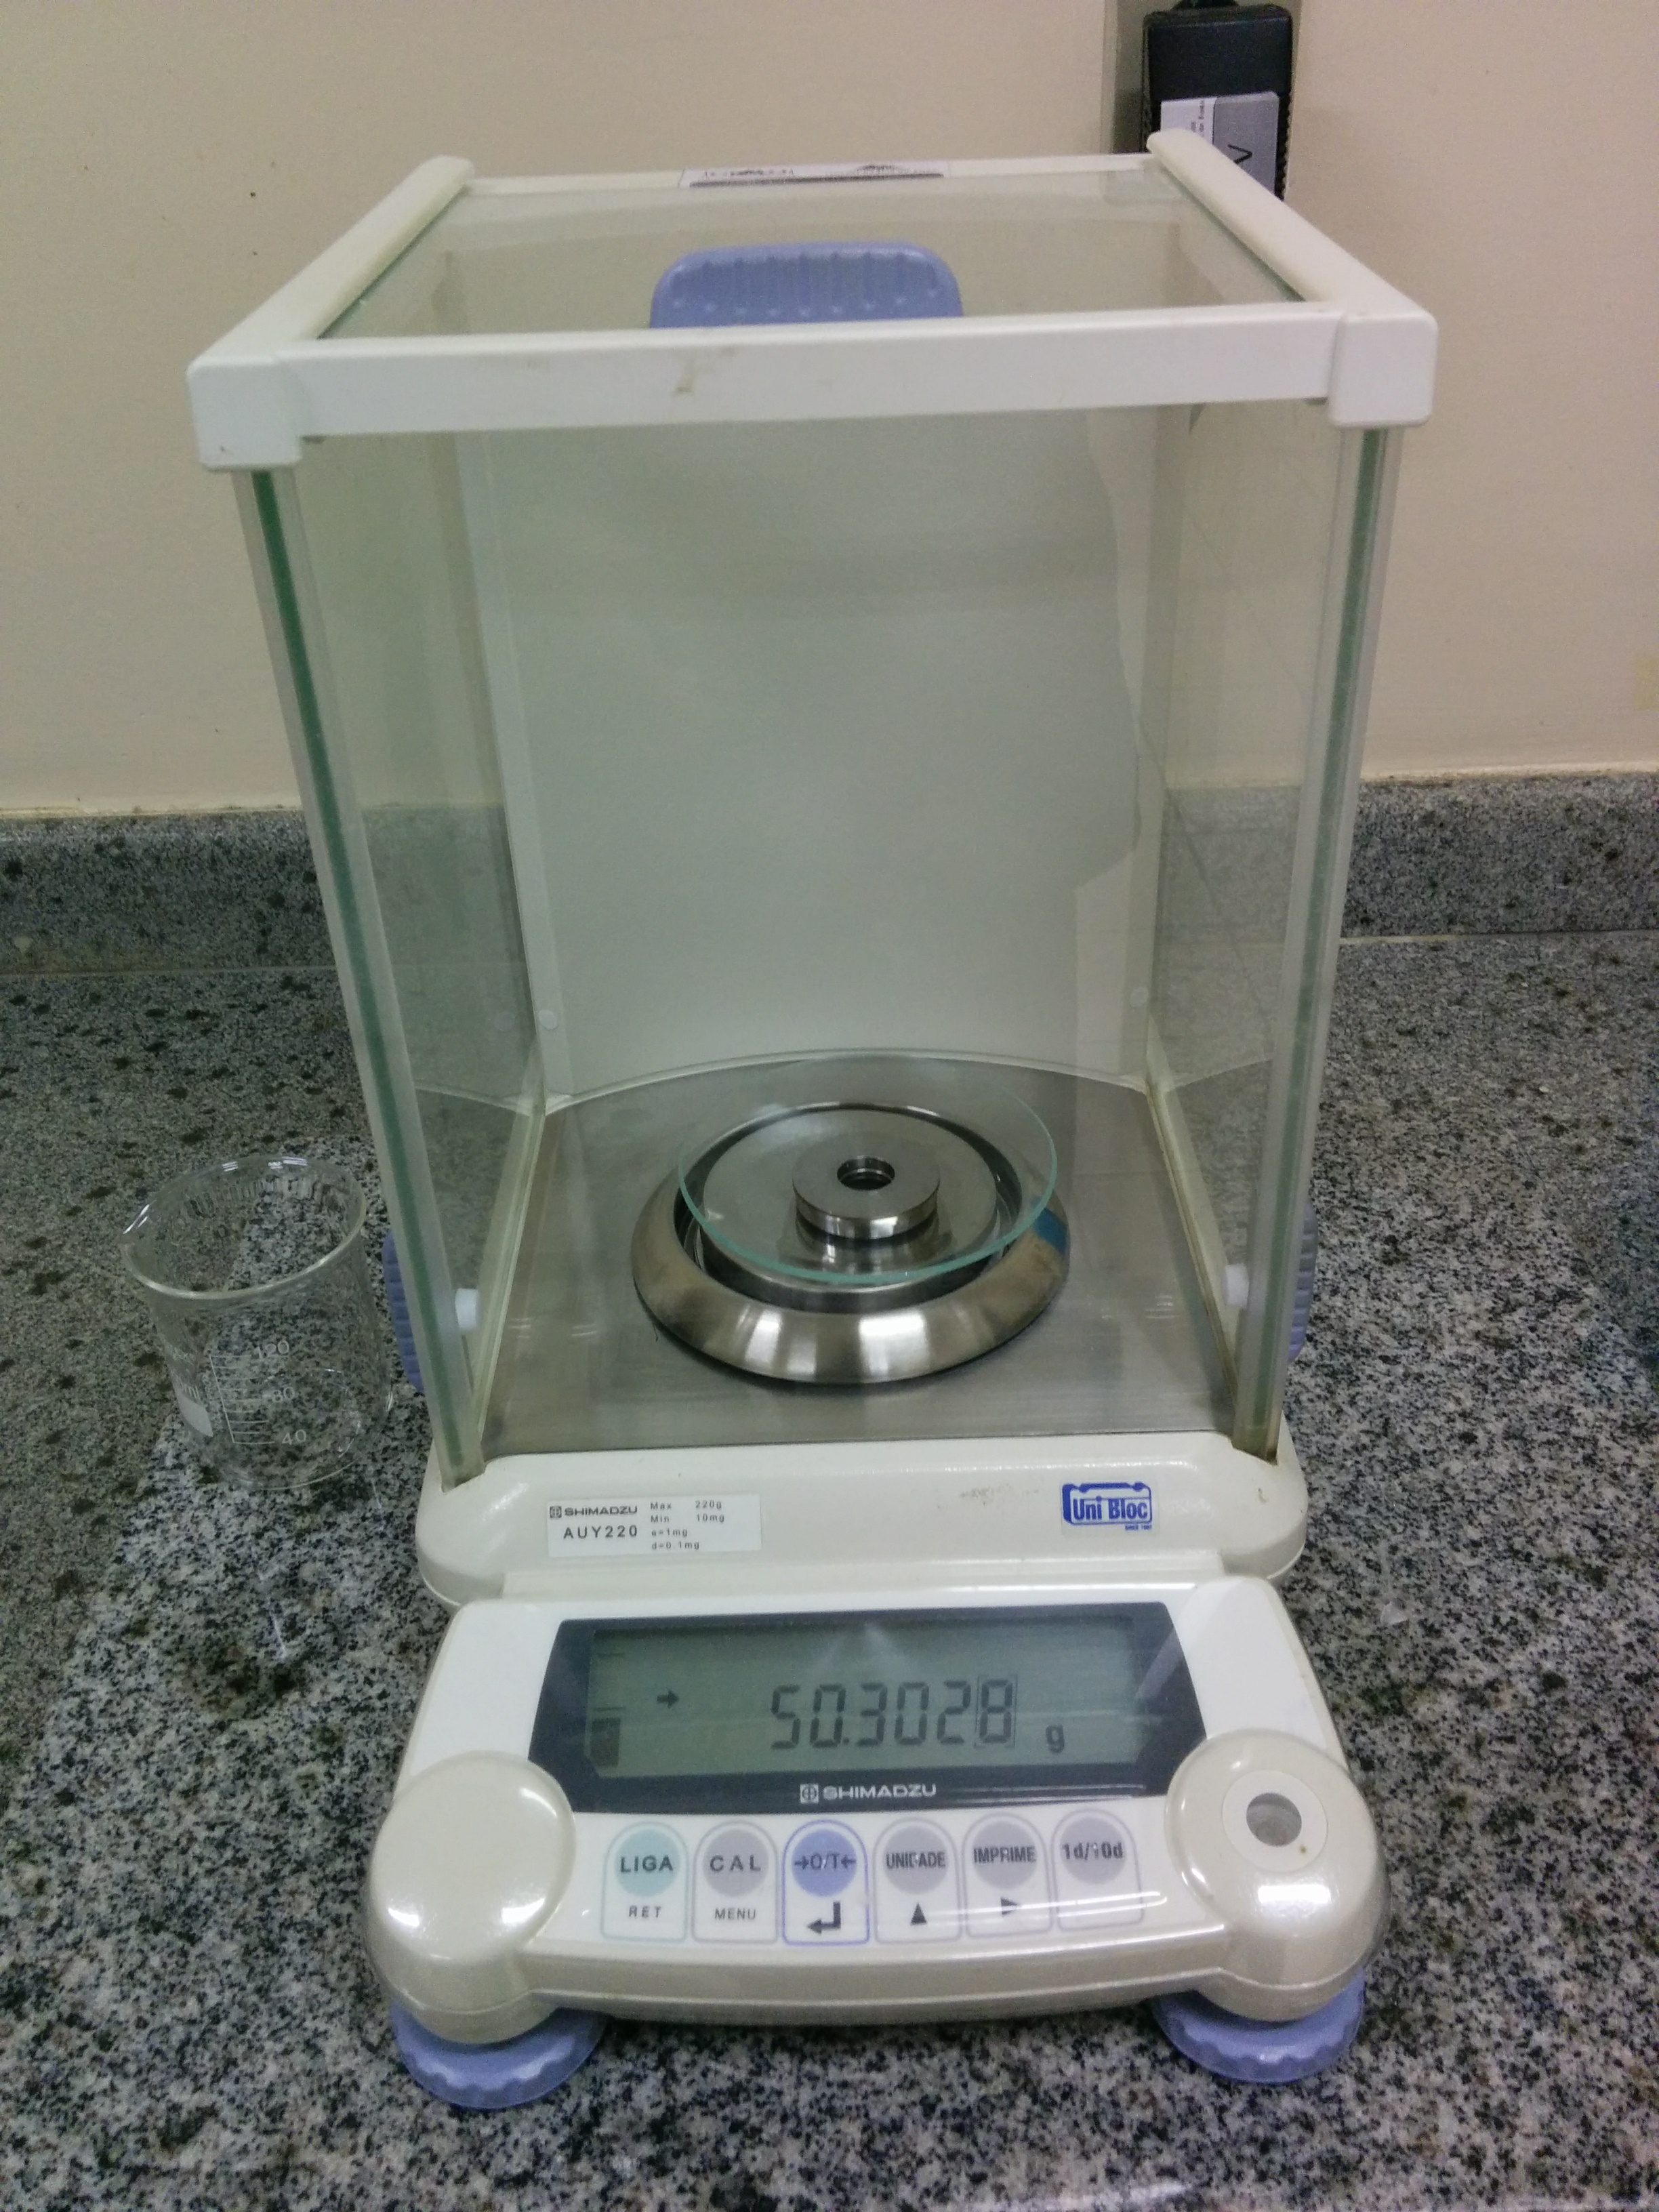
\includegraphics[width=0.5\textwidth]{balanca}
		\caption{Balança analítica utilizada nos procedimentos de pesagem.}
		\label{fig:balanca}
	\end{figure}

	Os dados de perda de massa e o cálculo de suas taxas de desgaste associadas obtidos em cada teste para cada amostra foram anotados para posterior análise. As tabelas, gráficos e análises dos dados obtidos com o teste de desgaste para todas as amostras analisadas, perlíticas e bainíticas, estão expostos na seção \ref{sec:ensaio_desgaste}.
	
	
	
\chapter{RESULTADOS E ANÁLISES}

\section{Análise de dureza}
\label{sec:analise_dureza}


\subsection{Dureza pós-austêmpera}
\label{sec:analise_dureza_pos_austempera}
	Os dados obtidos da realização dos testes de dureza pós-austêmpera das amostras perlíticas e bainíticas estão representados na Tab. \ref{tab:dureza_pos_austempera}.
	
	\begin{table}[H]
		\centering
		\caption{Leituras obtidas para as amostras perlíticas e para as amostras bainíticas (pós tratamento de austêmpera).}
		\begin{tabular}{|ccc|ccc|}
			\hline
			\multicolumn{6}{|c|}{Dureza (HRC)} \bigstrut\\
			\hline
			Amostra    & Leitura    & Média      & Amostra    & Leitura    & Média \bigstrut\\
			\hline
			\multirow{3}[2]{*}{Perlita 1} & 40         & \multirow{3}[2]{*}{40,3} & \multirow{3}[2]{*}{Bainita 1} & 59         & \multirow{3}[2]{*}{59,7} \bigstrut[t]\\
			& 40         &            &            & 60         &  \\
			& 41         &            &            & 60         &  \bigstrut[b]\\
			\hline
			\multirow{3}[2]{*}{Perlita 2} & 40         & \multirow{3}[2]{*}{40,3} & \multirow{3}[2]{*}{Bainita 2} & 42         & \multirow{3}[2]{*}{44,0} \bigstrut[t]\\
			& 40         &            &            & 45         &  \\
			& 41         &            &            & 45         &  \bigstrut[b]\\
			\hline
			\multirow{3}[2]{*}{Perlita 3} & 41         & \multirow{3}[2]{*}{40,7} & \multirow{3}[2]{*}{Bainita 3} & 56         & \multirow{3}[2]{*}{53,7} \bigstrut[t]\\
			& 41         &            &            & 52         &  \\
			& 40         &            &            & 53         &  \bigstrut[b]\\
			\hline
		\end{tabular}%
		\label{tab:dureza_pos_austempera}%
	\end{table}%
	
	Observa-se através dos resultados de dureza das amostra bainíticas que o tratamento de austêmpera elevou consideravelmente a dureza dessas amostras quando comparada a seus valores originais, que seriam próximos aos das amostras perlíticas.
	
\subsection{Dureza pós-revenido}
\label{sec:analise_dureza_pos_revenido}
	Os testes de dureza realizados nesta etapa tiveram o objetivo de assegurar que as durezas dos corpos de prova de bainita, que, conforme a Tab. \ref{tab:dureza_pos_austempera}, eram de 59,7 HRC, 44,0 HRC e 53,7 HRC, chegassem a valores próximos àqueles dos corpos perlíticos puros não tratados (aproximadamente 40,5 HRC, segundo a Tab. \ref{tab:dureza_pos_austempera}). 
	
	Os dados das medições de dureza dos corpos de bainita (pós-revenido) e de perlita; e das leituras de dureza para o contracorpo estão expressos na Tab. \ref{tab:dureza_pos_revenimento}.
	
	
	\begin{table}[H]
		\centering
		\caption{Valores de dureza obtidos para as amostras perlíticas, bainíticas pós-revenimento e para o contracorpo.}
		\resizebox{\textwidth}{!}{%
			\begin{tabular}{|ccc|ccc|ccc|}
				\hline
				\multicolumn{9}{|c|}{Dureza (HRC)} \bigstrut\\
				\hline
				Amostra & Leitura & Média & Amostra & Leitura & Média & Amostra & Leitura & Média \bigstrut\\
				\hline
				\multirow{4}[2]{*}{Perlita 1} & 40,0 & \multirow{4}[2]{*}{39,9} & \multirow{4}[2]{*}{Bainita 1} & 38,5 & \multirow{4}[2]{*}{40,5} & \multicolumn{1}{c}{\multirow{12}[6]{*}{Contracorpo}} & \multirow{3}[1]{*}{43,5} & \multirow{12}[6]{*}{41,3} \bigstrut[t]\\
				& 41,0 &   &   & 41,0 &   &   &   &  \\
				& 39,0 &   &   & 41,0 &   &   &   &  \\
				& 39,5 &   &   & 41,5 &   &   & \multirow{3}[2]{*}{40,0} &  \bigstrut[b]\\
				\cline{1-6}    \multirow{4}[2]{*}{Perlita 2} & 38,0 & \multirow{4}[2]{*}{39,6} & \multirow{4}[2]{*}{Bainita 2} & 38,0 & \multirow{4}[2]{*}{36,9} &   &   &  \bigstrut[t]\\
				& 39,0 &   &   & 37,0 &   &   &   &  \\
				& 40,0 &   &   & 36,5 &   &   & \multirow{3}[2]{*}{41,5} &  \\
				& 41,5 &   &   & 36,0 &   &   &   &  \bigstrut[b]\\
				\cline{1-6}    \multirow{4}[2]{*}{Perlita 3} & 40,5 & \multirow{4}[2]{*}{40,6} & \multirow{4}[2]{*}{Bainita 3} & 40,0 & \multirow{4}[2]{*}{40,9} &   &   &  \bigstrut[t]\\
				& 41,0 &   &   & 40,0 &   &   & \multirow{3}[1]{*}{40,0} &  \\
				& 41,0 &   &   & 41,0 &   &   &   &  \\
				& 40,0 &   &   & 42,5 &   &   &   &  \bigstrut[b]\\
				\hline
			\end{tabular}%
		}
		\label{tab:dureza_pos_revenimento}%
	\end{table}%
	
	É possível observar que o tratamento de revenimento realmente foi eficaz na redução de dureza dos três corpos de prova bainíticos. Considerando a escala Rockwell C, a amostra Bainita 1 teve sua dureza reduzida em 32\%, a Bainita 2, 16\%, e a Bainita 3, 24\%.
	
	O tratamento de revenimento das amostras bainíticas possibilitou a continuação dos estudos para a comparação de desempenho em desgaste entre as amostras perlíticas e bainíticas, pois promoveu a fixação de uma dureza comum dos corpos de prova.

\pagebreak
\section{Micrografia}
\label{sec:micrografia}

	Nesta seção estão expostas as imagens micrográficas realizadas de uma amostra bainítica e uma amostra perlítica, que foram cortadas estrategicamente para a observação e análise de suas superfícies. São apresentadas também comparações das imagens obtidas pela microscopia eletrônica de varredura com as imagens microestruturais clássicas presentes na literatura.

\subsection{Amostra bainítica}
\label{sec:micrografia_bainita}

	As Figuras \ref{fig:bainita_10_2}, \ref{fig:bainita_5_2} e \ref{fig:bainita_2_1} a seguir mostram as micrografias da amostra de teste bainítica com ampliação de 2000, 5000 e 7000 vezes, respectivamente.
	
	\begin{figure}[H]
		\centering
		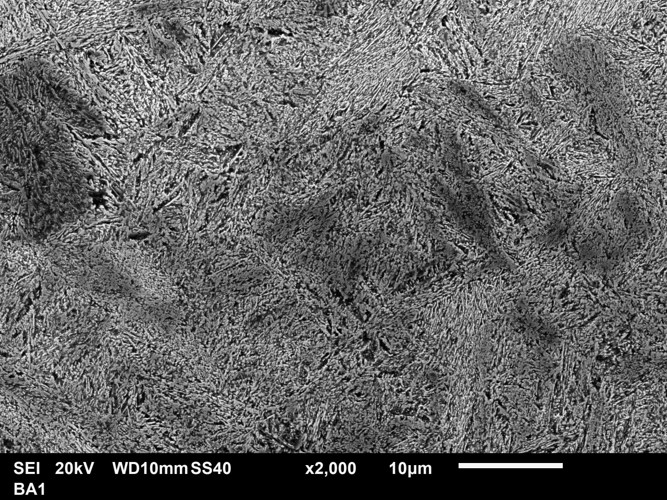
\includegraphics[width=1\textwidth]{bainita_10_2}
		\caption{Micrografia da amostra de teste bainítica com ampliação de 2000 vezes.}
		\label{fig:bainita_10_2}
	\end{figure}
	
	\begin{figure}[H]
		\centering
		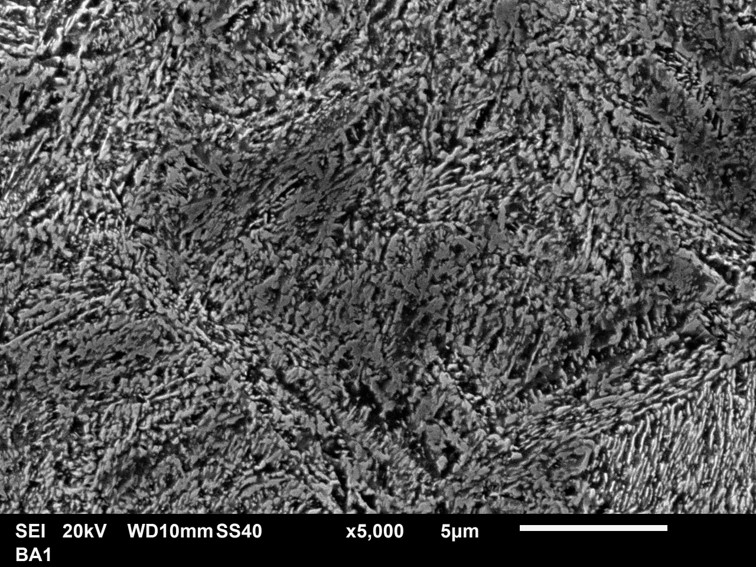
\includegraphics[width=0.9\textwidth]{bainita_5_2}
		\caption{Micrografia da amostra de teste bainítica com ampliação de 5000 vezes.}
		\label{fig:bainita_5_2}
	\end{figure}
	
	\begin{figure}[H]
		\centering
		\includegraphics[width=0.9\textwidth]{bainita_2_1}
		\caption{Micrografia da amostra de teste bainítica com ampliação de 7000 vezes.}
		\label{fig:bainita_2_1}
	\end{figure}
	
	Através das Figs. \ref{fig:bainita_5_2} e \ref{fig:bainita_2_1}, verifica-se que o revenimento, apesar de ter sido realizado em um curto período de tempo, foi suficiente para dar início ao processo de esferoidização da microestrutura em alguns pontos.
	
	Pela proximidade das imagens obtidas pela microscopia eletrônica de varredura com as imagens extraídas da literatura (Seção \ref{sec:imagens_bibliografia}), pode-se concluir que a formação da microestrutura bainítica após o revenido foi correta e, portanto, a austêmpera foi realizada de forma adequada. A Figura \ref{fig:comparacao_bainita} mostra em detalhes a comparação entre as Figs. \ref{fig:bainita_5_2} e \ref{fig:revenido_bib}.
	
	\begin{figure}[H]
		\centering
		\includegraphics[width=1\textwidth]{comparacao_bainita}
		\caption{Comparação entre a micrografia da parte superior, obtida da amostra de teste bainítica, e a micrografia inferior, presente na literatura, que representa um aço após o tratamento de revenimento.}
		\label{fig:comparacao_bainita}
	\end{figure}

\pagebreak
\subsection{Amostra perlítica}
\label{sec:micrografia_perlita}
	
	A Figura \ref{fig:perlita1000x} a seguir mostra a única micrografia feita da amostra de teste perlítica, com ampliação de 1000 vezes.
	
	\begin{figure}[H]
		\centering
		\includegraphics[width=1\textwidth]{perlita1000x}
		\caption{Micrografia da amostra de teste perlítica com ampliação de 1000 vezes.}
		\label{fig:perlita1000x}
	\end{figure}

	Como pode-se perceber, há uma grande semelhança entre as imagens da micrografia da amostra de teste perlítica obtidas por meio da microscopia eletrônica de varredura com as imagens clássicas de perlita encontradas na literatura (Seção \ref{sec:imagens_bibliografia}). É possível observar a presença de grãos de ferrita e cementita dispostos em lamelas e, portanto, condiz com o esperado para uma microestrutura perlítica. 
	
	A Figura \ref{fig:comparacao_perlita} mostra em detalhes a comparação entre as Figs. \ref{fig:perlita1000x} e \ref{fig:perlita_bib}.

\begin{figure}[H]
	\centering
	\includegraphics[width=1\textwidth]{comparacao_perlita}
	\caption{Comparação entre a micrografia superior, obtida da amostra de teste perlítica, e a micrografia inferior, presente na literatura, que representa um aço eutetóide com microestrutura perlítica.}
	\label{fig:comparacao_perlita}
\end{figure}


\pagebreak
\section{Ensaio de desgaste}
\label{sec:ensaio_desgaste}

	As Tabelas \ref{tab:perlita1}, \ref{tab:perlita2}, \ref{tab:bainita1} e \ref{tab:bainita2} abaixo mostram os dados obtidos com o teste de desgaste para todas as amostras, perlíticas e bainíticas, analisadas.

	\begin{table}[H]
		\centering
		\caption{Dados de perda de massa e taxa de desgaste obtidos a partir do ensaio de desgaste para a primeira amostra de perlita.}
		\resizebox{\textwidth}{!}{%
			\begin{tabular}{|ccccccc|}
				\hline
				\multicolumn{7}{|c|}{\textbf{Perlita 1}} \bigstrut\\
				\hline
				\multicolumn{1}{|p{3em}}{Carga} & \multicolumn{1}{p{3.5em}}{Leitura} & \multicolumn{1}{p{6.5em}}{Massa da amostra (g)} & \multicolumn{1}{p{6.5em}}{Perda de massa (g)} & \multicolumn{1}{p{7.5em}}{Taxa de desgaste (g.h/m)} & \multicolumn{1}{p{7.5em}}{Taxa de desgaste média (g.h/m)} & \multicolumn{1}{p{7.5em}|}{Desvio padrão (g.h/m)} \bigstrut\\
				\hline
				- & - & 59,7719 & - & - & - & - \bigstrut\\
				\hline
				\multirow{3}[2]{*}{5kg} & 1 & 59,7708 & 0,0011 & 5,78E-04 & \multirow{3}[2]{*}{4,03E-04} & \multirow{3}[2]{*}{2,19E-04} \bigstrut[t]\\
				& 2 & 59,7705 & 0,0003 & 1,58E-04 &   &  \\
				& 3 & 59,7696 & 0,0009 & 4,73E-04 &   &  \bigstrut[b]\\
				\hline
			\end{tabular}%
		}
		\label{tab:perlita1}%
	\end{table}%
	
	\begin{table}[H]
		\centering
		\caption{Dados de perda de massa e taxa de desgaste obtidos a partir do ensaio de desgaste para a segunda amostra de perlita.}
		\resizebox{\textwidth}{!}{%
			\begin{tabular}{|ccccccc|}
				\hline
				\multicolumn{7}{|c|}{\textbf{Perlita 2}} \bigstrut\\
				\hline
				\multicolumn{1}{|p{3em}}{Carga} & \multicolumn{1}{p{3.5em}}{Leitura} & \multicolumn{1}{p{6.5em}}{Massa da amostra (g)} & \multicolumn{1}{p{6.5em}}{Perda de massa (g)} & \multicolumn{1}{p{7.5em}}{Taxa de desgaste (g.h/m)} & \multicolumn{1}{p{7.5em}}{Taxa de desgaste média (g.h/m)} & \multicolumn{1}{p{7.5em}|}{Desvio padrão (g.h/m)} \bigstrut\\
				\hline
				- & - & 59,5556 & - & - & - & - \bigstrut\\
				\hline
				\multirow{3}[2]{*}{5kg} & 1 & 59,5538 & 0,0018 & 9,46E-04 & \multirow{3}[2]{*}{5,43E-04} & \multirow{3}[2]{*}{3,58E-04} \bigstrut[t]\\
				& 2 & 59,5533 & 0,0005 & 2,63E-04 &   &  \\
				& 3 & 59,5525 & 0,0008 & 4,20E-04 &   &  \bigstrut[b]\\
				\hline
			\end{tabular}%
		}
		\label{tab:perlita2}%
	\end{table}%
	
	\begin{table}[H]
		\centering
		\caption{Dados de perda de massa e taxa de desgaste obtidos a partir do ensaio de desgaste para a primeira amostra de bainita.}
		\resizebox{\textwidth}{!}{%
			\begin{tabular}{|ccccccc|}
				\hline
				\multicolumn{7}{|c|}{\textbf{Bainita 1}} \bigstrut\\
				\hline
				\multicolumn{1}{|p{3em}}{Carga} & \multicolumn{1}{p{3.5em}}{Leitura} & \multicolumn{1}{p{6.5em}}{Massa da amostra (g)} & \multicolumn{1}{p{6.5em}}{Perda de massa (g)} & \multicolumn{1}{p{7.5em}}{Taxa de desgaste (g.h/m)} & \multicolumn{1}{p{7.5em}}{Taxa de desgaste média (g.h/m)} & \multicolumn{1}{p{7.5em}|}{Desvio padrão (g.h/m)} \bigstrut\\
				\hline
				- & - & 53,4592 & - & - & - & - \bigstrut\\
				\hline
				\multirow{3}[2]{*}{5kg} & 1 & 53,4581 & 0,0011 & 5,78E-04 & \multirow{3}[2]{*}{8,76E-04} & \multirow{3}[2]{*}{2,70E-04} \bigstrut[t]\\
				& 2 & 53,456 & 0,0021 & 1,10E-03 &   &  \\
				& 3 & 53,4542 & 0,0018 & 9,46E-04 &   &  \bigstrut[b]\\
				\hline
			\end{tabular}%
		}
		\label{tab:bainita1}%
	\end{table}%
	
	\begin{table}[H]
		\centering
		\caption{Dados de perda de massa e taxa de desgaste obtidos a partir do ensaio de desgaste para a segunda amostra de bainita.}
		\resizebox{\textwidth}{!}{%
			\begin{tabular}{|ccccccc|}
				\hline
				\multicolumn{7}{|c|}{\textbf{Bainita 2}} \bigstrut\\
				\hline
				\multicolumn{1}{|p{3em}}{Carga} & \multicolumn{1}{p{3.5em}}{Leitura} & \multicolumn{1}{p{6.5em}}{Massa da amostra (g)} & \multicolumn{1}{p{6.5em}}{Perda de massa (g)} & \multicolumn{1}{p{7.5em}}{Taxa de desgaste (g.h/m)} & \multicolumn{1}{p{7.5em}}{Taxa de desgaste média (g.h/m)} & \multicolumn{1}{p{7.5em}|}{Desvio padrão (g.h/m)} \bigstrut\\
				\hline
				- & - & 50,3032 & - & - & - & - \bigstrut\\
				\hline
				\multirow{3}[2]{*}{5kg} & 1 & 50,3028 & 0,0004 & 2,10E-04 & \multirow{3}[2]{*}{2,63E-04} & \multirow{3}[2]{*}{5,25E-05} \bigstrut[t]\\
				& 2 & 50,3023 & 0,0005 & 2,63E-04 &   &  \\
				& 3 & 50,3017 & 0,0006 & 3,15E-04 &   &  \bigstrut[b]\\
				\hline
			\end{tabular}%
		}
		\label{tab:bainita2}%
	\end{table}%




	O gráfico da Fig. \ref{fig:graf1} expressa os dados de taxas de desgaste das Tabelas \ref{tab:perlita1}, \ref{tab:perlita2}, \ref{tab:bainita1} e \ref{tab:bainita2} de forma visualizável.
	\begin{figure}[H]
		\centering
		\includegraphics[width=1\textwidth]{graf1}
		\caption{Reprodução dos dados de desgaste obtidos a partir do ensaio de desgaste em forma de gráfico.}
		\label{fig:graf1}
	\end{figure}

	Como pode-se observar, as taxas de desgaste apresentaram valores bastante variáveis, mesmo quando analisando cada amostra individualmente, não apresentando assim, uma constância de resultados, com exceção da amostra Bainita 2. Também não foi possível segregar as amostras bainíticas das perlíticas por taxa de desgaste maior ou menor. Até mesmo dentro da mesma categoria de microestrutura os resultados são divergentes, por exemplo as amostras Bainita 1 e Bainita 2 são ambas bainíticas e apresentam, respectivamente, a maior e menor média de desgaste de todas as amostras analisadas.
	
	A Figura \ref{fig:graf2} mostra um gráfico onde cada símbolo representa a média dos três testes de cada amostra e as barras representam o desvio padrão.

	\begin{figure}[H]
		\centering
		\includegraphics[width=1\textwidth]{graf2}
		\caption{Gráfico da média dos testes de cada amostra com barras representando o desvio padrão das taxas de desgastes individuais. Os números próximos aos símbolos representam a dureza de cada amostra.}
		\label{fig:graf2}
	\end{figure}

	Através das longas barras verticais é possível notar o alto desvio padrão de taxas de desgaste para uma mesma amostra; a única exceção é a amostra Bainita 2, que apresentou taxas de desgaste relativamente constantes para todos os testes.
	
	Sendo as amostras mais macias do que o trilho, que possui 41,3 HRC - Tab. \ref{tab:dureza_pos_revenimento}, as amostras são os materiais que devem desgastar mais rapidamente. Segundo a equação de Archard (Eq. \ref{eq:archard}), a taxa de desgaste é inversamente proporcional a dureza de um material, porém esse fato também não se evidencia nos resultados da Fig. \ref{fig:graf2}, já que a amostra que possui a maior dureza de todas analisadas (Bainita 1) possui também a maior taxa de desgaste, enquanto que a amostra mais macia de todas (Bainita 2) apresentou a menor taxa de desgaste entre todas, mesmo com relação àquelas com microestruturas iguais.

\chapter{CONCLUSÕES}
		A partir das análises dos resultados das Figs. \ref{fig:graf1} e \ref{fig:graf2} é possível deduzir que o método de avaliação de desgaste adotado não é adequado. Tal inconformidade de resultados pode ter ocorrido pelos seguintes motivos:
		
		\begin{enumerate}[label=\roman*]
			\item As tensões aplicadas entre o contato roda-trilho é muito baixa: A espessura da área de rolamento foi reduzida a 2 mm através usinagem de chanfros na pista de rolamento e a carga utilizada foi a da massa de 5 kg, maior massa disponível no laboratório para o tribômetro. Apesar disso, as tensões impostas nos corpos de provas, mesmo em miniaturas, são muito inferiores a tais percebidas em aplicações reais no transporte de minério de ferro. Com tensões próximas às tensões reais, as perdas de massa poderia ser bem mais significativas;
			
			\item A balança não possui precisão necessária: As aferições de massa foram realizadas em balanças analíticas, com precisão de 0,0001 g. Todavia, é possível que as perdas de massa por desgaste para a carga aplicada sejam tão ínfimas que não possam ser perfeitamente captadas pela balança;
			
			\item O ambiente externo interfere na massa da amostra: Como as perdas de massa são muito pequenas, a própria interação do ambiente com o corpo de prova pode alterar sua massa. Tal interação prejudica a observação da perda de massa por desgaste. Apesar de ser sido realizada a lavagem ultrassônica em todos os corpos de prova antes da aferição de massa, a amostra pode, com mais ou menos intensidade, ter adquirido partículas do ar ou dos dedos do manuseador no deslocamento da lavadora até a balança. Além disso, outro fenômeno de interação com o ambiente que ocorre e pode resultar em alterações de massa é a oxidação gradual do metal com o ar atmosférico;
			
			\item O tempo de rolamento não é suficiente: O intervalo de teste adotado no tribômetro foi de 1 hora. Esse intervalo de tempo pode não ser suficiente para uma perda de massa por desgaste significativa. Uma maior perda de massa por desgaste através do aumento do tempo de teste reduziria a influência de outras variáveis na variação da massa;
			
			\item Desgaste de forma aleatória: O fenômeno de desgaste ocorreu de forma não linear. As massas perdidas através das tensões do contato roda-trilho não foram constantes. Detritos maiores podem se quebrar da amostra de forma repentina, assim como durante um longo intervalo pode nenhuma partícula se soltar. Para reduzir esses efeitos na avaliação do real desgaste, longos intervalos de tempo de testes seriam necessários.
			
		\end{enumerate}
	
	As diferentes microestruturas, bainítica e perlítica, podem ser melhor comparadas e avaliadas com relação a seus desempenhos em desgaste através das propostas de melhorias mencionadas. O estudo da tribologia e da análise de desgaste, especialmente no contato roda-trilho, apesar de envolver fenômenos complexos e, em certo grau, imprevisíveis, não deve ser negligenciado, pois estudos nessa área afetam diretamente a confiabilidade e segurança de sistemas mecânicos. Além disso, máquinas e mecanismos que sofrem menos falhas ou que têm seus tempos entre falhas reduzidos auxiliam no sentido de minimizar custos com manutenção corretiva e preventiva em empresas e consequentemente aumentar a produtividade e competitividade dessas no mercado.
%% ----------------------------------------------------------
%% ELEMENTOS POS-TEXTUAIS
	
\postextual
	
%% Referencias. LISTAR EXATAMENTE AS CITADAS NO TRABALHO.
\bibliographystyle{abbrv}
\bibliography{referencias}



\begin{anexosenv}
	
	
	\chapter{TERMO DE AUTENTICIDADE}
	
	%\begin{folhadeaprovacao}
	\begin{figure}[h]
		\centering
		\includegraphics[scale=0.75]{01.png}
	\end{figure}
	\begin{center}
		\textbf{Termo de Declaração de Autenticidade de Autoria}\\
		\vfill
		%		{\chapterfont \bfseries \insereautor}
		%		
		%		\vfill
		%		\begin{center}
		%			{\chapterfont\bfseries\inseretitulo \inseresubtitulo}
	\end{center}
	%		\vfill
	
	\noindent Declaro, sob as penas da lei e para os devidos fins, junto à Universidade Federal de Juiz de Fora, que meu Trabalho de Conclusão de Curso do Curso de Graduação em Engenharia Mecânica é original, de minha única e exclusiva autoria. E não se trata de cópia integral ou parcial de textos e trabalhos de autoria de outrem, seja em formato de papel, eletrônico, digital, áudio-visual ou qualquer outro meio.
	
	\noindent Declaro ainda ter total conhecimento e compreensão do que é considerado plágio, não apenas a cópia integral do trabalho, mas também de parte dele, inclusive de artigos e/ou parágrafos, sem citação do autor ou de sua fonte. 
	
	\noindent Declaro, por fim, ter total conhecimento e compreensão das punições decorrentes da prática de plágio, através das sanções civis previstas na lei do direito autoral\footnote{{\footnotesize LEI N$\mathrm{^\circ}$ 9.610, DE 19 DE FEVEREIRO DE 1998. Altera, atualiza e consolida a legislação sobre direitos autorais e dá outras providências.}}  e criminais previstas no Código Penal\footnote{{\footnotesize Art. 184. Violar direitos de autor e os que lhe são conexos: Pena – detenção, de 3 (três) meses a 1 (um) ano, ou multa.}}, além das cominações administrativas e acadêmicas que poderão resultar em reprovação no Trabalho de Conclusão de Curso. 
	
	\vfill
	
	\begin{center}
		Juiz de Fora, 19 de julho de 2018.
	\end{center}
	
	\vfill
	
	\assinatura{Henrique Abrantes Vitoi \\ Matrícula: 201271035  -- CPF: 107.676.696-06} 
	
	\vspace{30mm}
	
	
\end{anexosenv}
	

	%%% ---
\end{document}
